
\title{Addendum to the Report on the ITER Clite Shutdown Dose rate Calculations}
\author{
  Andrew Davis \\
  Department of Engineering Physics\\
  College of Engineering \\
  The University of Wisconsin-Madison\\
  Madison, Wisconsin, 53706, \underline{USA}
  \and
  Mohamed Sawan \\
  Department of Engineering Physics\\
  College of Engineering \\
  The University of Wisconsin-Madison\\
  Madison, Wisconsin, 53706, \underline{USA}
  \and
  Paul P. H. Wilson \\
  Department of Engineering Physics\\
  College of Engineering \\
  The University of Wisconsin-Madison\\
  Madison, Wisconsin, 53706, \underline{USA}
  \and
  Elliott Biondo \\
  Department of Engineering Physics\\
  College of Engineering \\
  The University of Wisconsin-Madison\\
  Madison, Wisconsin, 53706, \underline{USA}
  \and
  Ahmad Ibrahim \\
  Radiation Transport Group\\
  Oak Ridge National Laboratory \\
  P.O. Box 2008 \\
  Oak Ridge, Tennessee 37831, \underline{USA}
  \and
  Patrick Shriwise \\
  Department of Engineering Physics\\
  College of Engineering \\
  The University of Wisconsin-Madison\\
  Madison, Wisconsin, 53706, \underline{USA}
  \and
  Edward Marriott\\
  Department of Engineering Physics\\
  College of Engineering \\
  The University of Wisconsin-Madison\\
  Madison, Wisconsin, 53706, \underline{USA}
}

\date{\today}

\documentclass[12pt]{article}
\usepackage{times}
\usepackage{graphicx}
\usepackage{longtable}
\usepackage[acronym]{glossaries}
\usepackage[a4paper, portrait, margin=0.5in]{geometry}
\usepackage[table]{xcolor}
\usepackage[nottoc,numbib]{tocbibind}
\usepackage{subcaption}
\usepackage{multirow}
\usepackage{draftwatermark}
\usepackage[hidelinks]{hyperref}

\SetWatermarkText{DRAFT}
\SetWatermarkScale{1}

%% define this page left blank
\newcommand*{\blankpage}{%
\vspace*{\fill}
\begin{center}
 \centering \textbf{This page intentionally left blank}
\end{center}
\vspace{\fill}}

%% to get lof in toc
\renewcommand{\listoffigures}{\begingroup
\tocsection
\tocfile{\listfigurename}{lof}
\endgroup}

%% to get lot in toc
\renewcommand{\listoftables}{\begingroup
\tocsection
\tocfile{\listtablename}{lot}
\endgroup}

\begin{document}
\maketitle
\newpage
\tableofcontents
\newpage
\listoffigures
\newpage
\listoftables
\newpage
\section{Introduction}
The original report \cite{iter_sdr_report} contained results for the baseline
ITER SA-2 irradiation scenario, included in this report are the two remaining
scenarios a reduced scenario where 10 years of operation has been removed, named
ITER SA-2 - 10 y,  and a reduced irradiation scenario where 5 years of operation
has been removed, named ITER SA-2 - 5 y.
\\
\\
The models and parameters for transport and activation are entirely unchanged 
and only differ by the irradiation scenario used, which is detailed in Section
\ref{sec:irradiation_scenario}
\newpage
\section{Irradiation Scenarios}
\label{sec:irradiation_scenario}
The following irradiation scenarios are the standard SA-2 scenario and 
two reduced versions of the ITER SA-2.
irradiation scenarios \cite{sa2_irradiation}. 
\subsection{ITER SA-2 Full}
\begin{table}[ht!]
   \begin{tabular}{| l | c | c | c |}
      \hline 
      Irradiation Period & Neutron Power (MW) & Source Normalisation (n/s) &  Relative Strength \\
      \hline
      2 Years & 2.7 & $1.061\times10^{17}$ & 0.0053 \\
      10 Years & 20.6 & $8.517\times10^{17}$ & 0.0412 \\
      0.667 Years & 0.0 & 0.0 & 0.0 \\
      1.325 Years & 41.5 & $1.643\times10^{18}$ & 0.0830 \\
      \cellcolor{blue!25} 3920 Seconds & \cellcolor{blue!25} 0.0 & \cellcolor{blue!25} 0.0 & \cellcolor{blue!25} 0.0 \\
      \cellcolor{blue!25} \cellcolor{blue!25} 400 Seconds & \cellcolor{blue!25} 500.0 & \cellcolor{blue!25} $1.973\times10^{19}$ & \cellcolor{blue!25} 1.0  \\
      \cellcolor{green!25} 3920 Seconds & \cellcolor{green!25} 0.0 & \cellcolor{green!25} 0.0 &\cellcolor{green!25} 0.0 \\
      \cellcolor{green!25} 400 Seconds & \cellcolor{green!25} 700.0 & \cellcolor{green!25} $2.772\times10^{19}$ &\cellcolor{green!25} 1.4 \\
      \hline
\end{tabular}
\caption{The table shows the SA-2 scenario for irradiation, note the
         cells in \textcolor{blue!25}{blue} are repeated 17 times
         and the cells in \textcolor{green!25}{green} are repeated 3
         times.}
\label{tab:irrad_scenario}
\end{table}
\subsection{ITER SA-2 - 5 year}
\begin{table}[ht!]
   \begin{tabular}{| l | c | c | c |}
      \hline 
      Irradiation Period & Neutron Power (MW) & Source Normalisation (n/s) &  Relative Strength \\
      \hline
      2 Years & 2.7 & $1.061\times10^{17}$ & 0.0053 \\
      5 Years & 20.6 & $8.517\times10^{17}$ & 0.0412 \\
      0.667 Years & 0.0 & 0.0 & 0.0 \\
      1.325 Years & 41.5 & $1.643\times10^{18}$ & 0.0830 \\
      \cellcolor{blue!25} 3920 Seconds & \cellcolor{blue!25} 0.0 & \cellcolor{blue!25} 0.0 & \cellcolor{blue!25} 0.0 \\
      \cellcolor{blue!25} \cellcolor{blue!25} 400 Seconds & \cellcolor{blue!25} 500.0 & \cellcolor{blue!25} $1.973\times10^{19}$ & \cellcolor{blue!25} 1.0  \\
      \cellcolor{green!25} 3920 Seconds & \cellcolor{green!25} 0.0 & \cellcolor{green!25} 0.0 &\cellcolor{green!25} 0.0 \\
      \cellcolor{green!25} 400 Seconds & \cellcolor{green!25} 700.0 & \cellcolor{green!25} $2.772\times10^{19}$ &\cellcolor{green!25} 1.4 \\
      \hline
\end{tabular}
\caption{The table shows the SA-2 - 5 year scenario for irradiation, note the
         cells in \textcolor{blue!25}{blue} are repeated 17 times
         and the cells in \textcolor{green!25}{green} are repeated 3
         times.}
\end{table}
\subsection{ITER SA-2 - 10 year}
\begin{table}[ht!]
   \begin{tabular}{| l | c | c | c |}
      \hline 
      Irradiation Period & Neutron Power (MW) & Source Normalisation (n/s) &  Relative Strength \\
      \hline
      2 Years & 2.7 & $1.061\times10^{17}$ & 0.0053 \\
      0.667 Years & 0.0 & 0.0 & 0.0 \\
      1.325 Years & 41.5 & $1.643\times10^{18}$ & 0.0830 \\
      \cellcolor{blue!25} 3920 Seconds & \cellcolor{blue!25} 0.0 & \cellcolor{blue!25} 0.0 & \cellcolor{blue!25} 0.0 \\
      \cellcolor{blue!25} \cellcolor{blue!25} 400 Seconds & \cellcolor{blue!25} 500.0 & \cellcolor{blue!25} $1.973\times10^{19}$ & \cellcolor{blue!25} 1.0  \\
      \cellcolor{green!25} 3920 Seconds & \cellcolor{green!25} 0.0 & \cellcolor{green!25} 0.0 &\cellcolor{green!25} 0.0 \\
      \cellcolor{green!25} 400 Seconds & \cellcolor{green!25} 700.0 & \cellcolor{green!25} $2.772\times10^{19}$ &\cellcolor{green!25} 1.4 \\
      \hline
\end{tabular}
\caption{The table shows the SA-2 - 10 year scenario for irradiation, note the
         cells in \textcolor{blue!25}{blue} are repeated 17 times
         and the cells in \textcolor{green!25}{green} are repeated 3
         times.}
\end{table}

\newpage
\section{Shutdown Photon Transport Results}
\label{sec:sdr_results}
\subsection{No B$_4$C}
\label{sec:sdr_results_nob4c}
The detailed transport data are contained within Appendix C for the ``SA-2 - 10'' irradiation
and Appendix D for the ``SA-2 - 5'' year irradiation. The data for the ``SA-2 - 10'' irradiation scenario
at the first decay time - 1$\times$10$^5$ s are shown in Figure \ref{fig:photons_5y_dc1_nob4c_dose} with the
associated relative error in Figure \ref{fig:photons_5y_dc1_nob4c_relerr}, the second
decay time - 1$\times$10$^6$ s are shown in Figure \ref{fig:photons_5y_dc2_nob4c_dose} with the
associated relative error in Figure \ref{fig:photons_5y_dc2_nob4c_relerr} and for the
third decay times - 1$\times$10$^7$ s are shown in Figure \ref{fig:photons_5y_dc3_nob4c_dose} with the
associated relative error in Figure \ref{fig:photons_5y_dc3_nob4c_relerr}. Detailed line outs
through the decay data are shown are in Figure \ref{fig:photons_5y_nob4c_dose}.
\\
\\
The data for the ``SA-2 - 5'' irradiation scenario
at the first decay time - 1$\times$10$^5$ s are shown in Figure \ref{fig:photons_10y_dc1_nob4c_dose} with the
associated relative error in Figure \ref{fig:photons_10y_dc1_nob4c_relerr}, the second
decay time - 1$\times$10$^6$ s are shown in Figure \ref{fig:photons_10y_dc2_nob4c_dose} with the
associated relative error in Figure \ref{fig:photons_10y_dc2_nob4c_relerr} and for the
third decay times - 1$\times$10$^7$ s are shown in Figure \ref{fig:photons_10y_dc3_nob4c_dose} with the
associated relative error in Figure \ref{fig:photons_10y_dc3_nob4c_relerr}. Detailed line outs
through the decay data are shown are in Figure \ref{fig:photons_10y_nob4c_dose}.
\newpage
\begin{figure}[ht!]
\centering
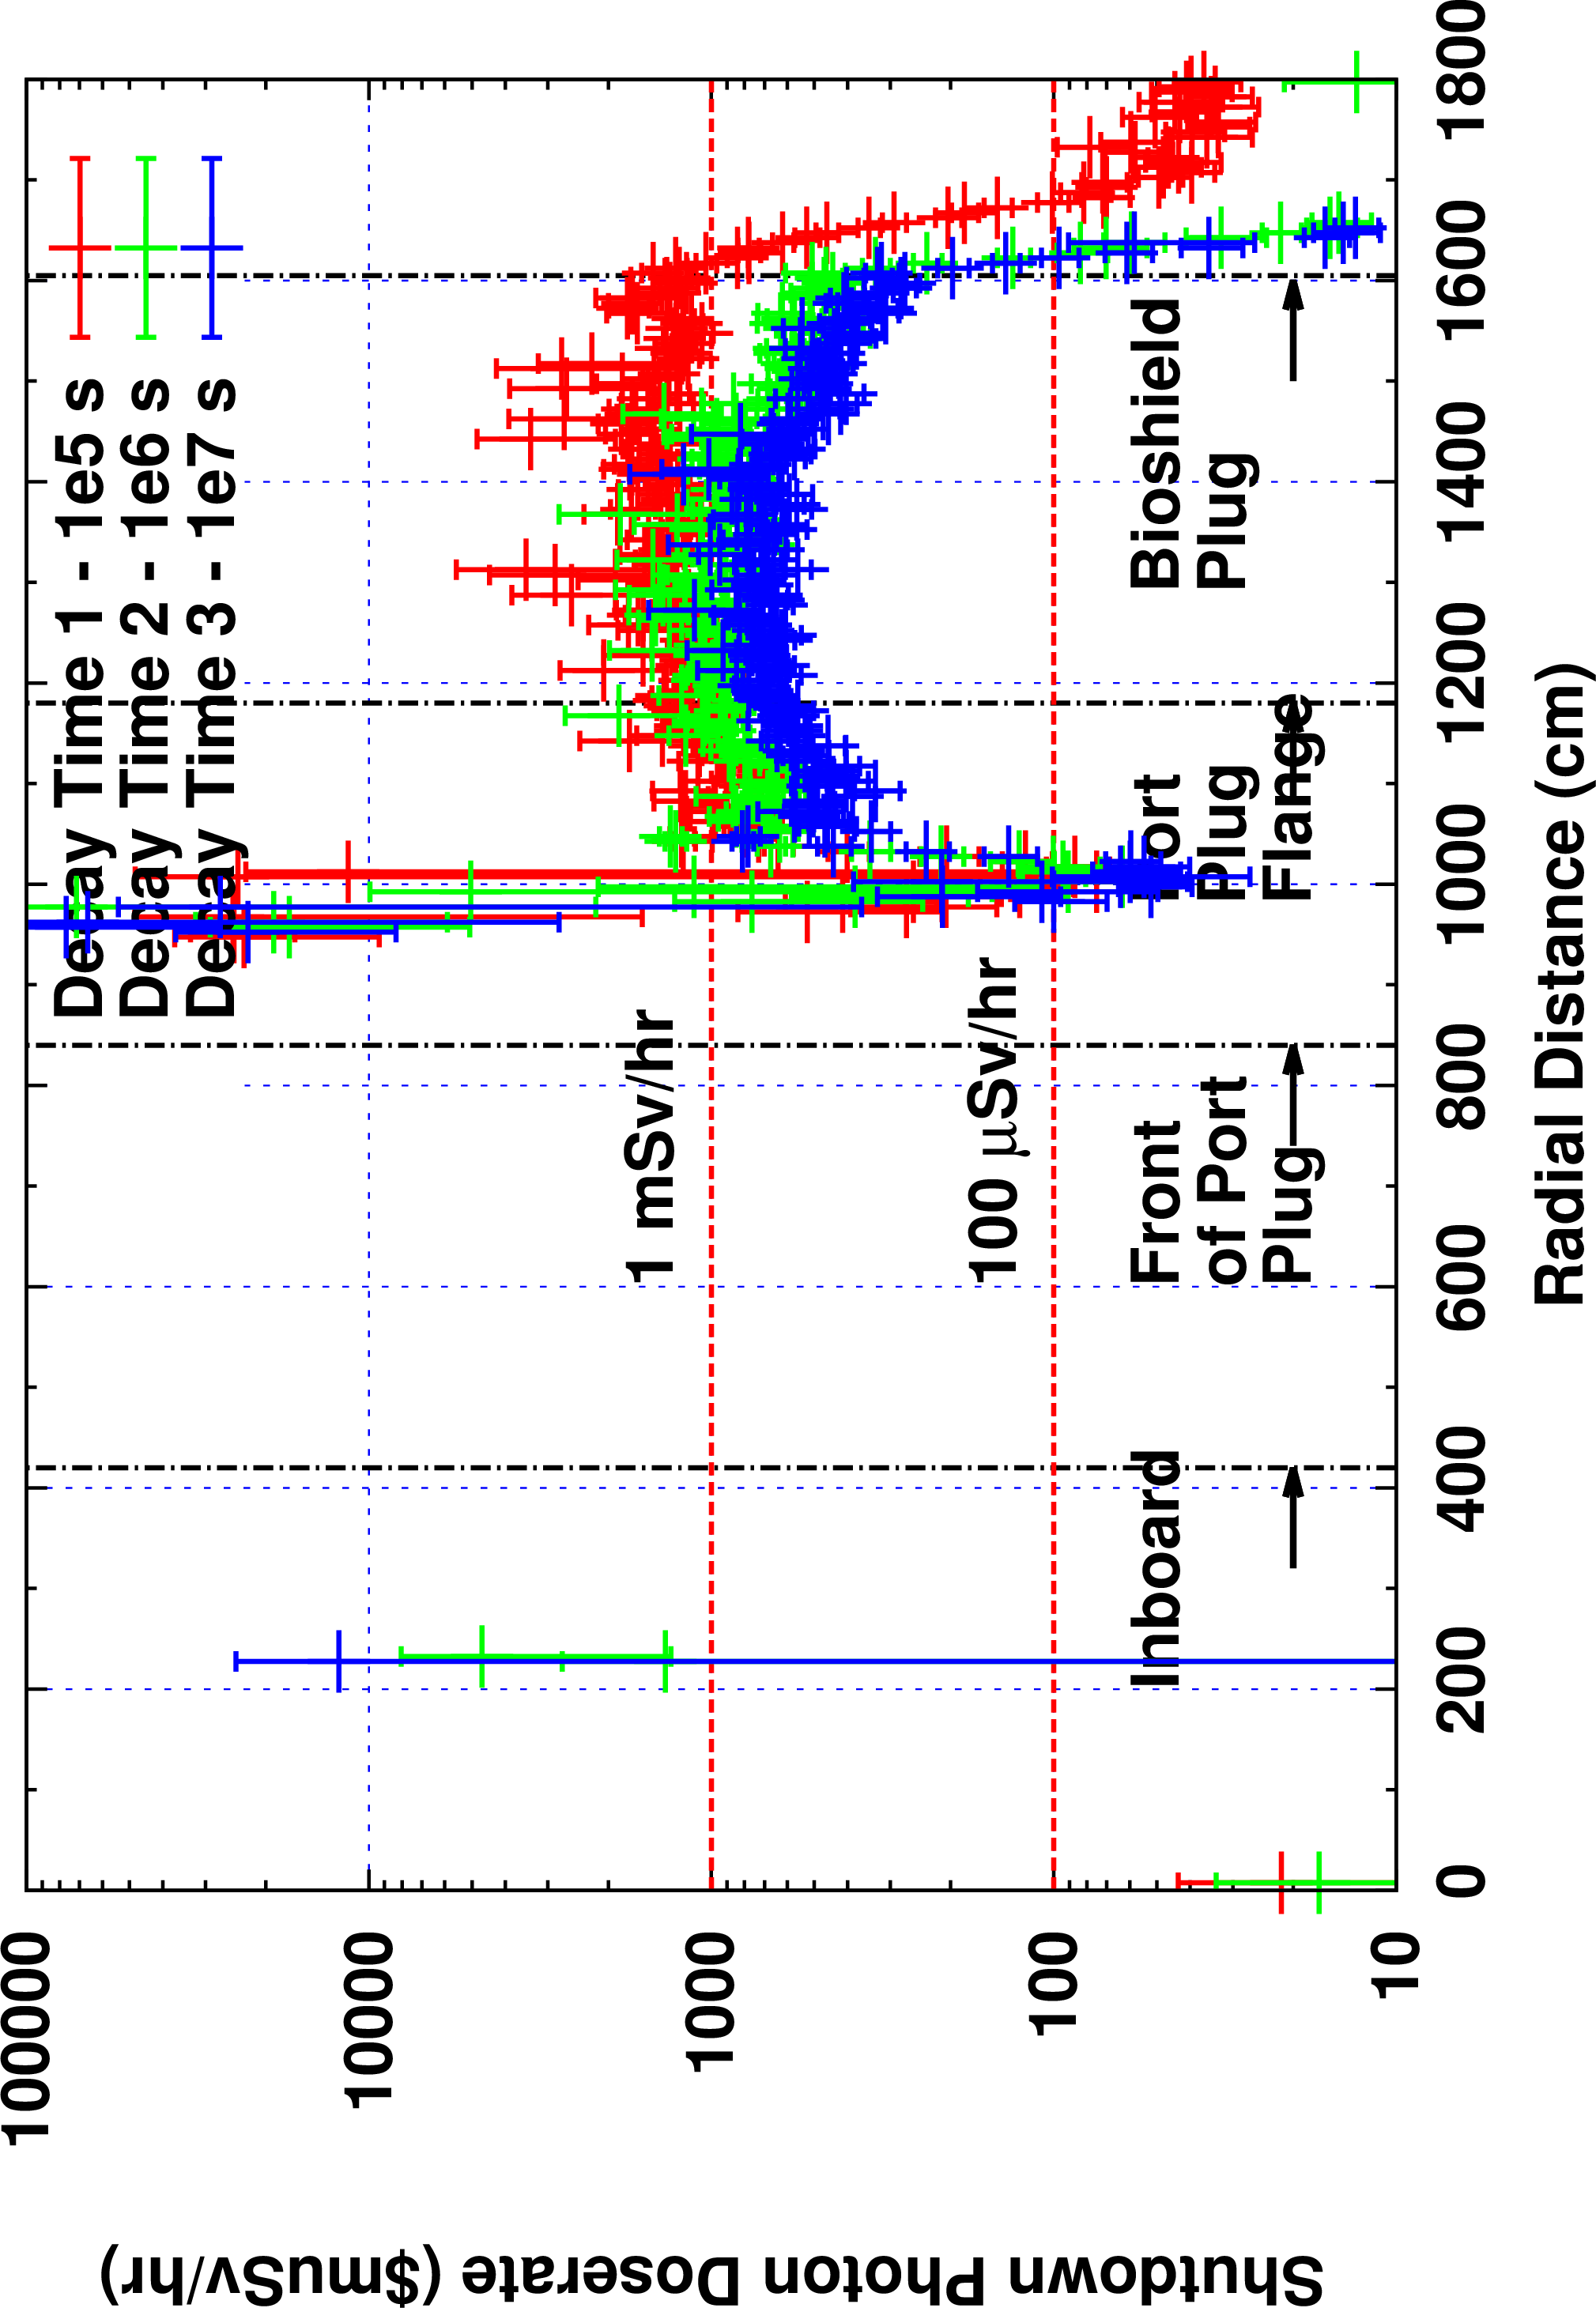
\includegraphics[clip,scale=0.12,angle=-90]{../plots/photon_lineout/5yr/no-b4c_5yr.png}
\caption{Total dose rate line from 0,0,60 to 1800,0,60 cm for the ``SA-2 - 10'' irradiation}
\label{fig:photons_5y_nob4c_dose}
\end{figure}
\begin{figure}[ht!]
\centering
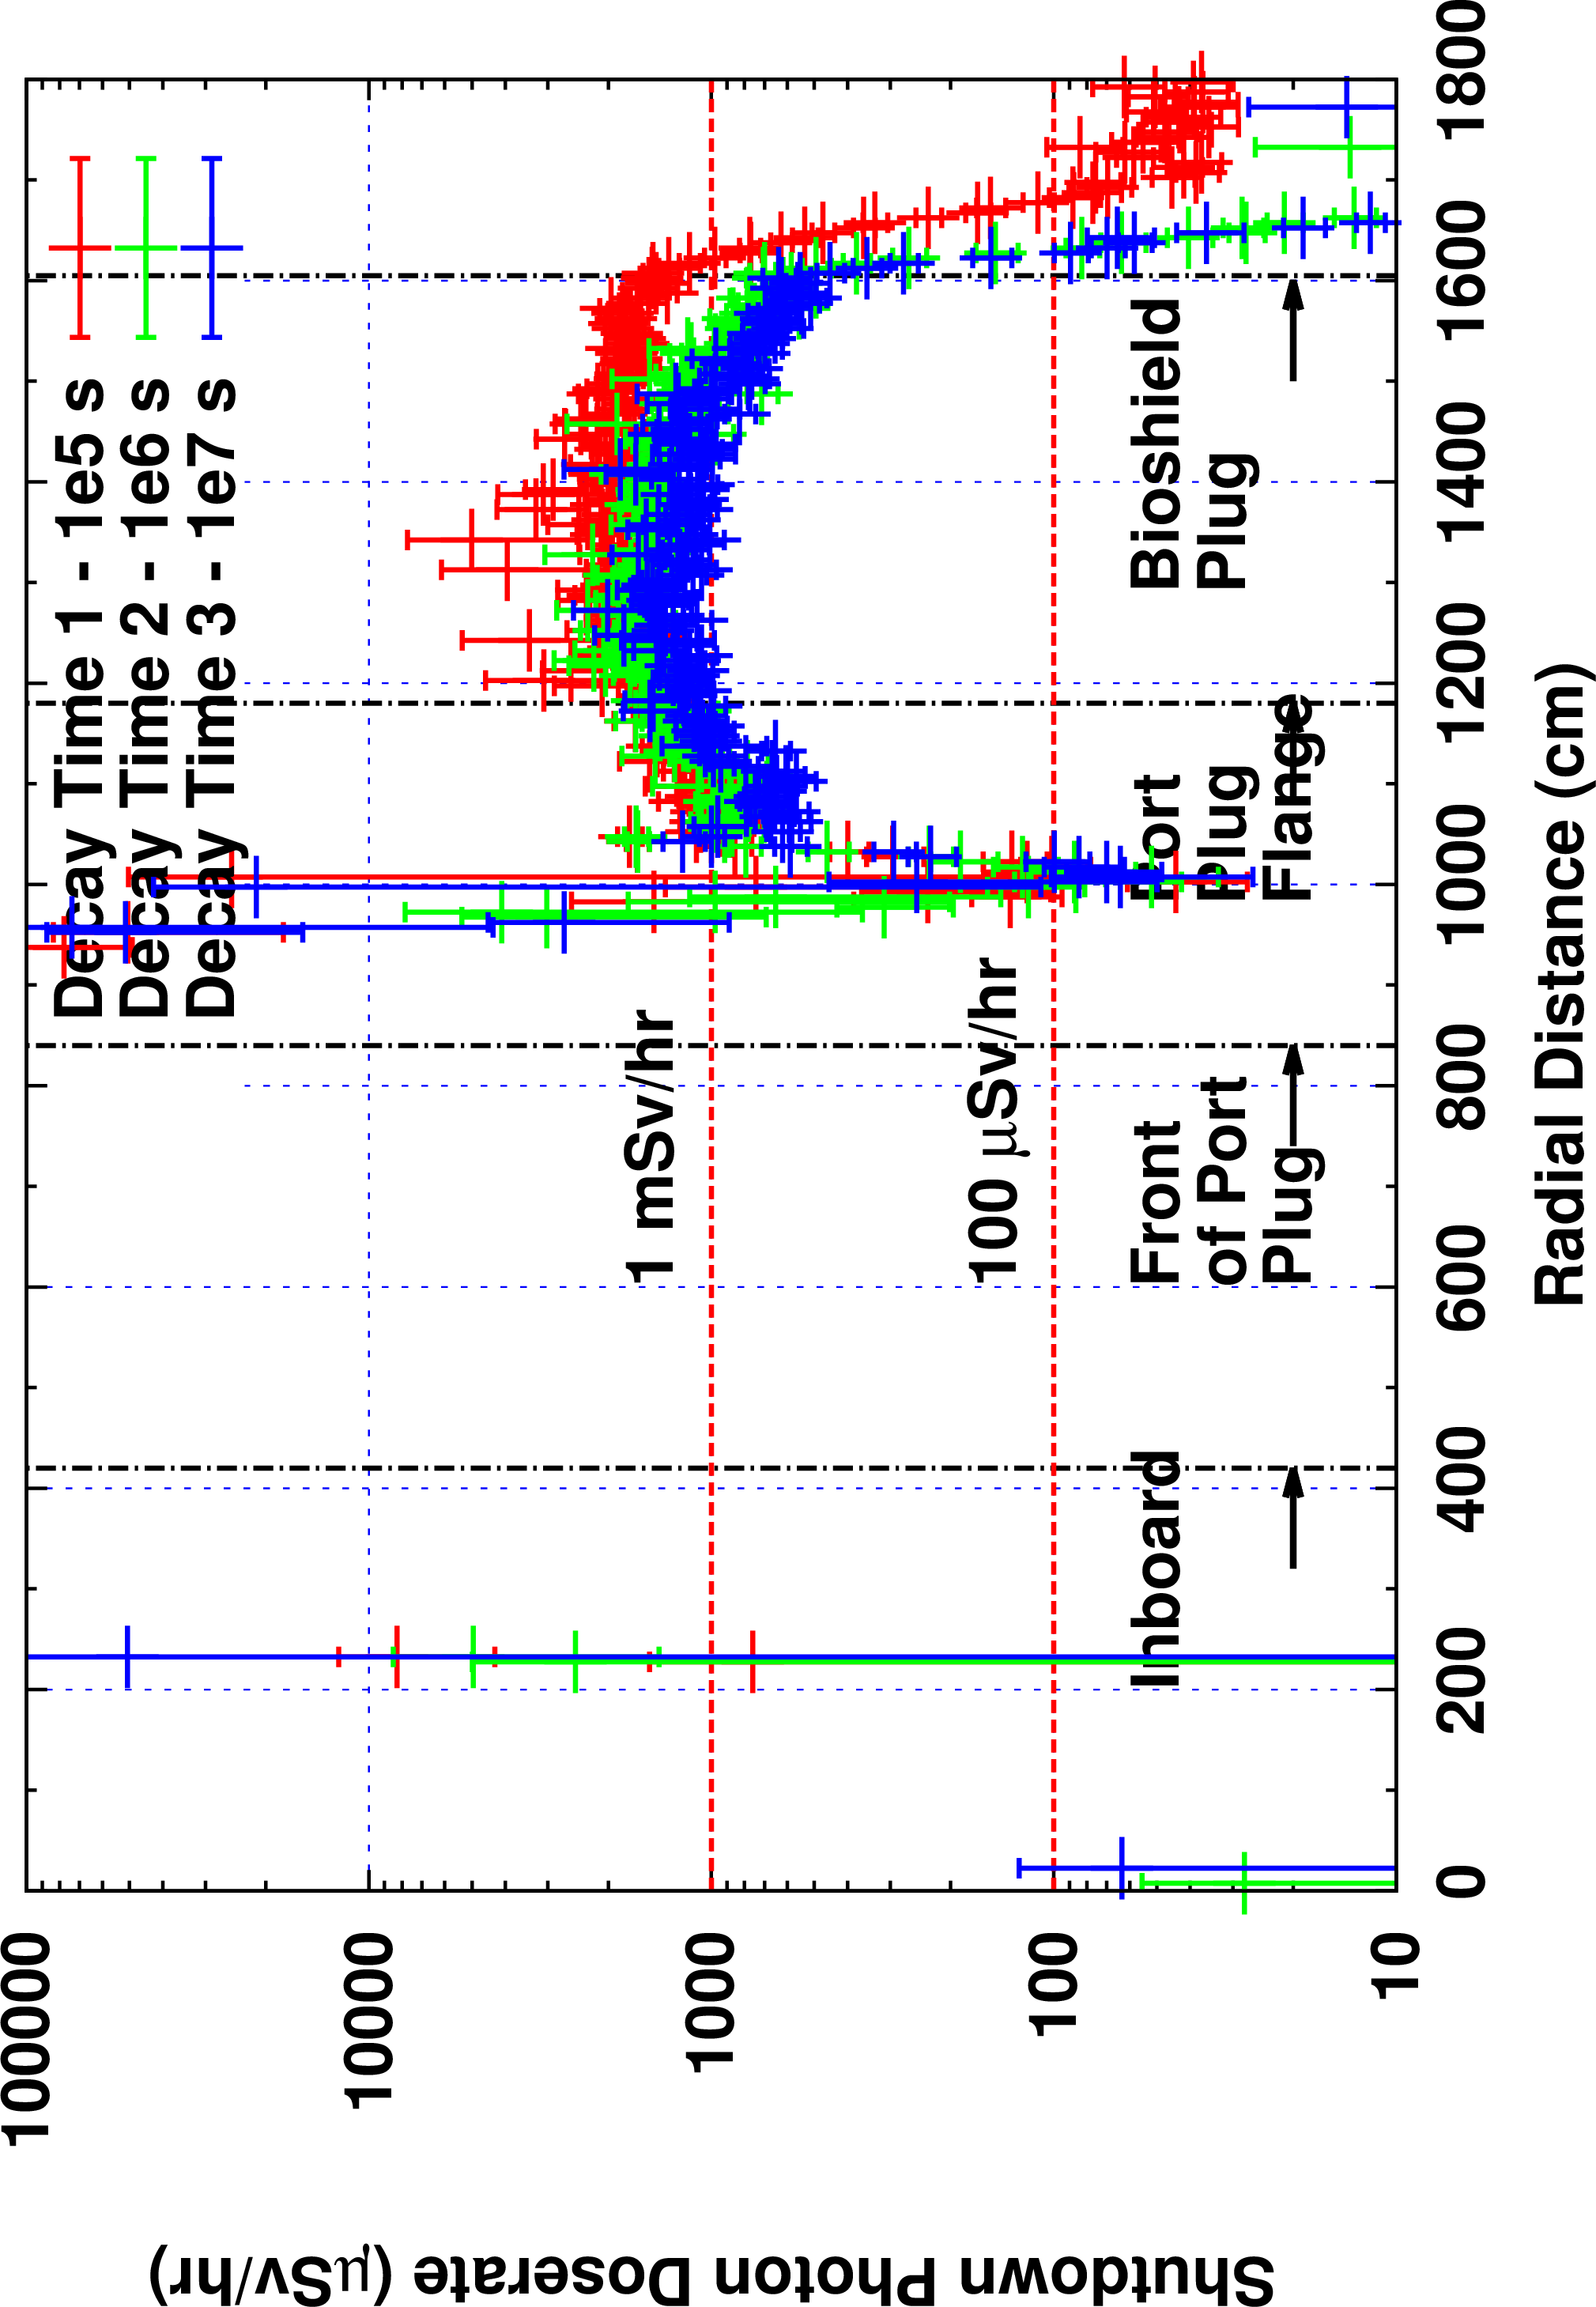
\includegraphics[clip,scale=0.12,angle=-90]{../plots/photon_lineout/10yr/no-b4c_10yr.png}
\caption{Total dose rate line line from 0,0,60 to 1800,0,60 cm for the ``SA-2 - 5'' irradiation}
\label{fig:photons_10y_nob4c_dose}
\end{figure}
\clearpage
\newpage
\subsection{B$_4$C}
\label{sec:sdr_results_b4c}
The detailed transport data are contained within Appendix A for the ``SA-2 - 10'' irradiation
and Appendix B for the ``SA-2 - 5'' irradiation. The data for the ``SA-2 - 10'' irradiation scenario
at the first decay time - 1$\times$10$^5$ s are shown in Figure \ref{fig:photons_5y_dc1_b4c_dose} with the
associated relative error in Figure \ref{fig:photons_5y_dc1_b4c_relerr}, the second
decay time - 1$\times$10$^6$ s are shown in Figure \ref{fig:photons_5y_dc2_b4c_dose} with the
associated relative error in Figure \ref{fig:photons_5y_dc2_b4c_relerr} and for the
third decay times - 1$\times$10$^7$ s are shown in Figure \ref{fig:photons_5y_dc3_b4c_dose} with the
associated relative error in Figure \ref{fig:photons_5y_dc3_b4c_relerr}. Detailed line outs
through the decay data are shown are in Figure \ref{fig:photons_5y_b4c_dose}.
\\
\\
The data for the ``SA-2 - 5'' irradiation scenario
at the first decay time - 1$\times$10$^5$ s are shown in Figure \ref{fig:photons_10y_dc1_b4c_dose} with the
associated relative error in Figure \ref{fig:photons_10y_dc1_b4c_relerr}, the second
decay time - 1$\times$10$^6$ s are shown in Figure \ref{fig:photons_10y_dc2_b4c_dose} with the
associated relative error in Figure \ref{fig:photons_10y_dc2_b4c_relerr} and for the
third decay times - 1$\times$10$^7$ s are shown in Figure \ref{fig:photons_10y_dc3_b4c_dose} with the
associated relative error in Figure \ref{fig:photons_10y_dc3_b4c_relerr}. Detailed line outs
through the decay data are shown are in Figure \ref{fig:photons_10y_b4c_dose}.
\newpage
\begin{figure}[ht!]
\centering
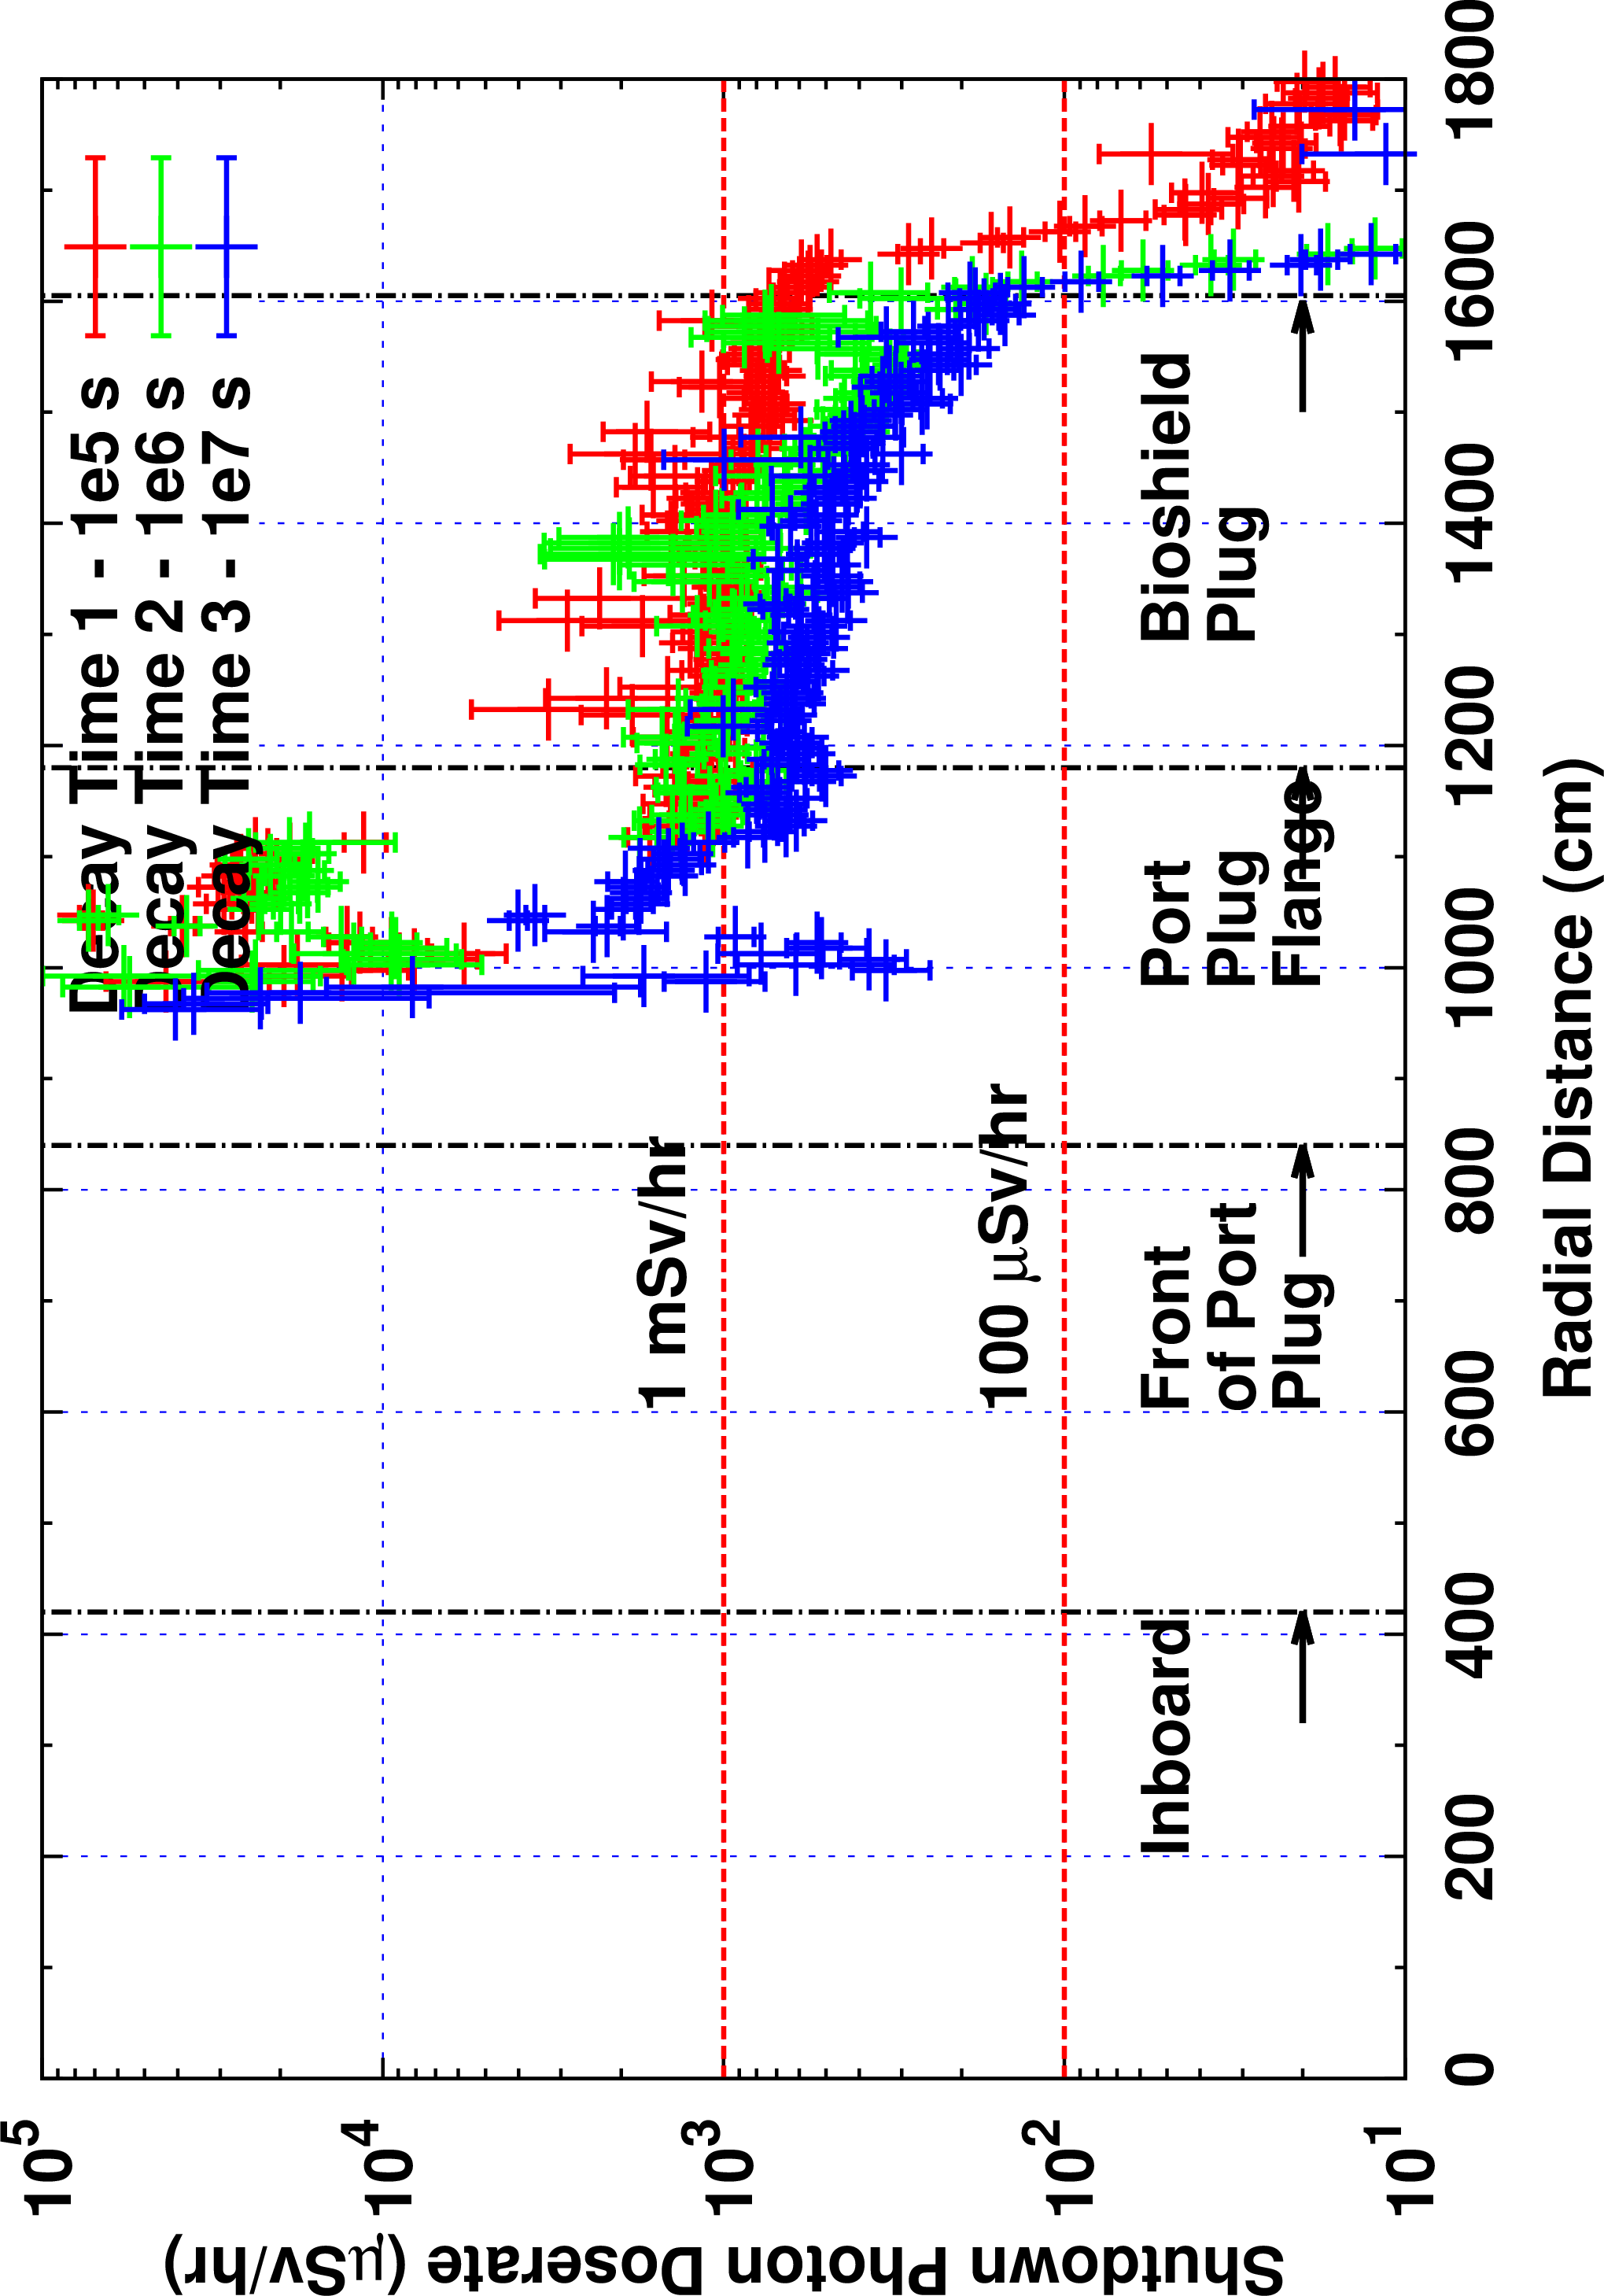
\includegraphics[clip,scale=0.12,angle=-90]{../plots/photon_lineout/5yr/b4c_5yr.png}
\caption{Total dose rate line from 0,0,60 to 1800,0,60 cm for the ``SA-2 - 10'' irradiation}
\label{fig:photons_5y_b4c_dose}
\end{figure}
\begin{figure}[ht!]
\centering
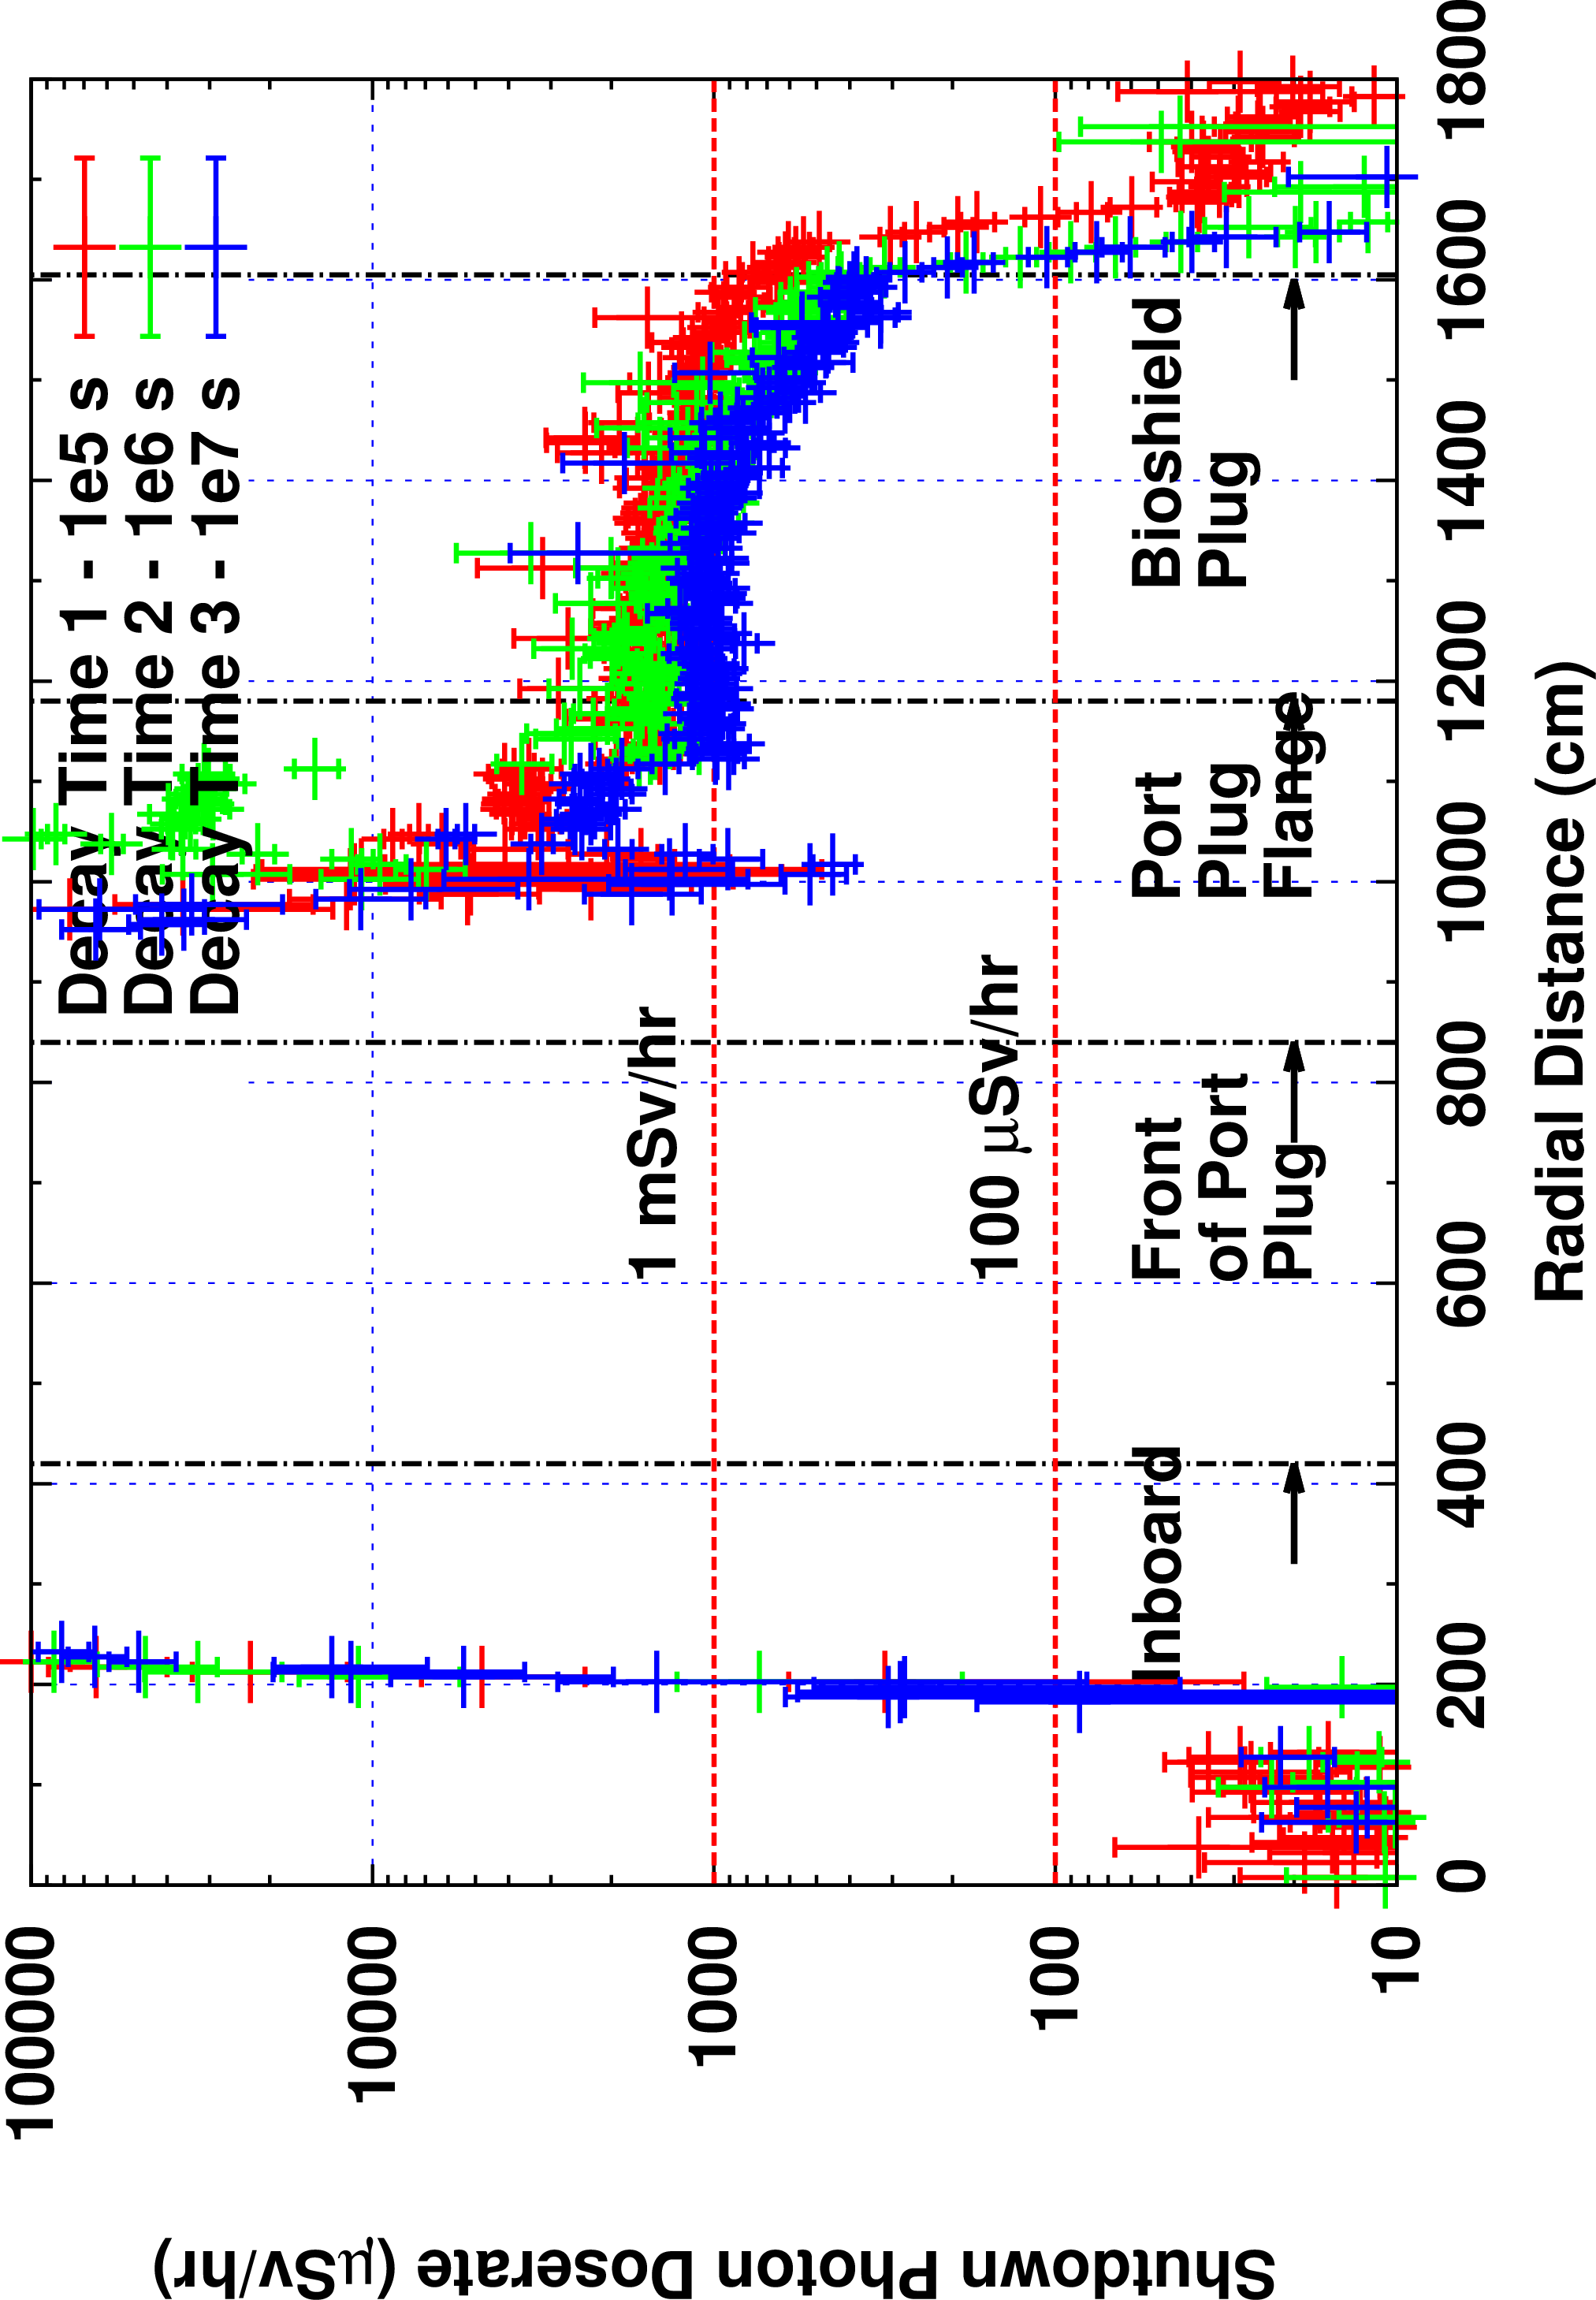
\includegraphics[clip,scale=0.12,angle=-90]{../plots/photon_lineout/10yr/b4c_10yr.png}
\caption{Total dose rate line line from 0,0,60 to 1800,0,60 cm for the ``SA-2 - 5'' irradiation}
\label{fig:photons_10y_b4c_dose}
\end{figure}

\clearpage
\newpage
\subsection{B$_4$C/No B$_4$C Comparison}
\subsubsection{Decay Time 1 - 1$\times$10$^{5}$ s}
\begin{figure}[ht!]
\centering
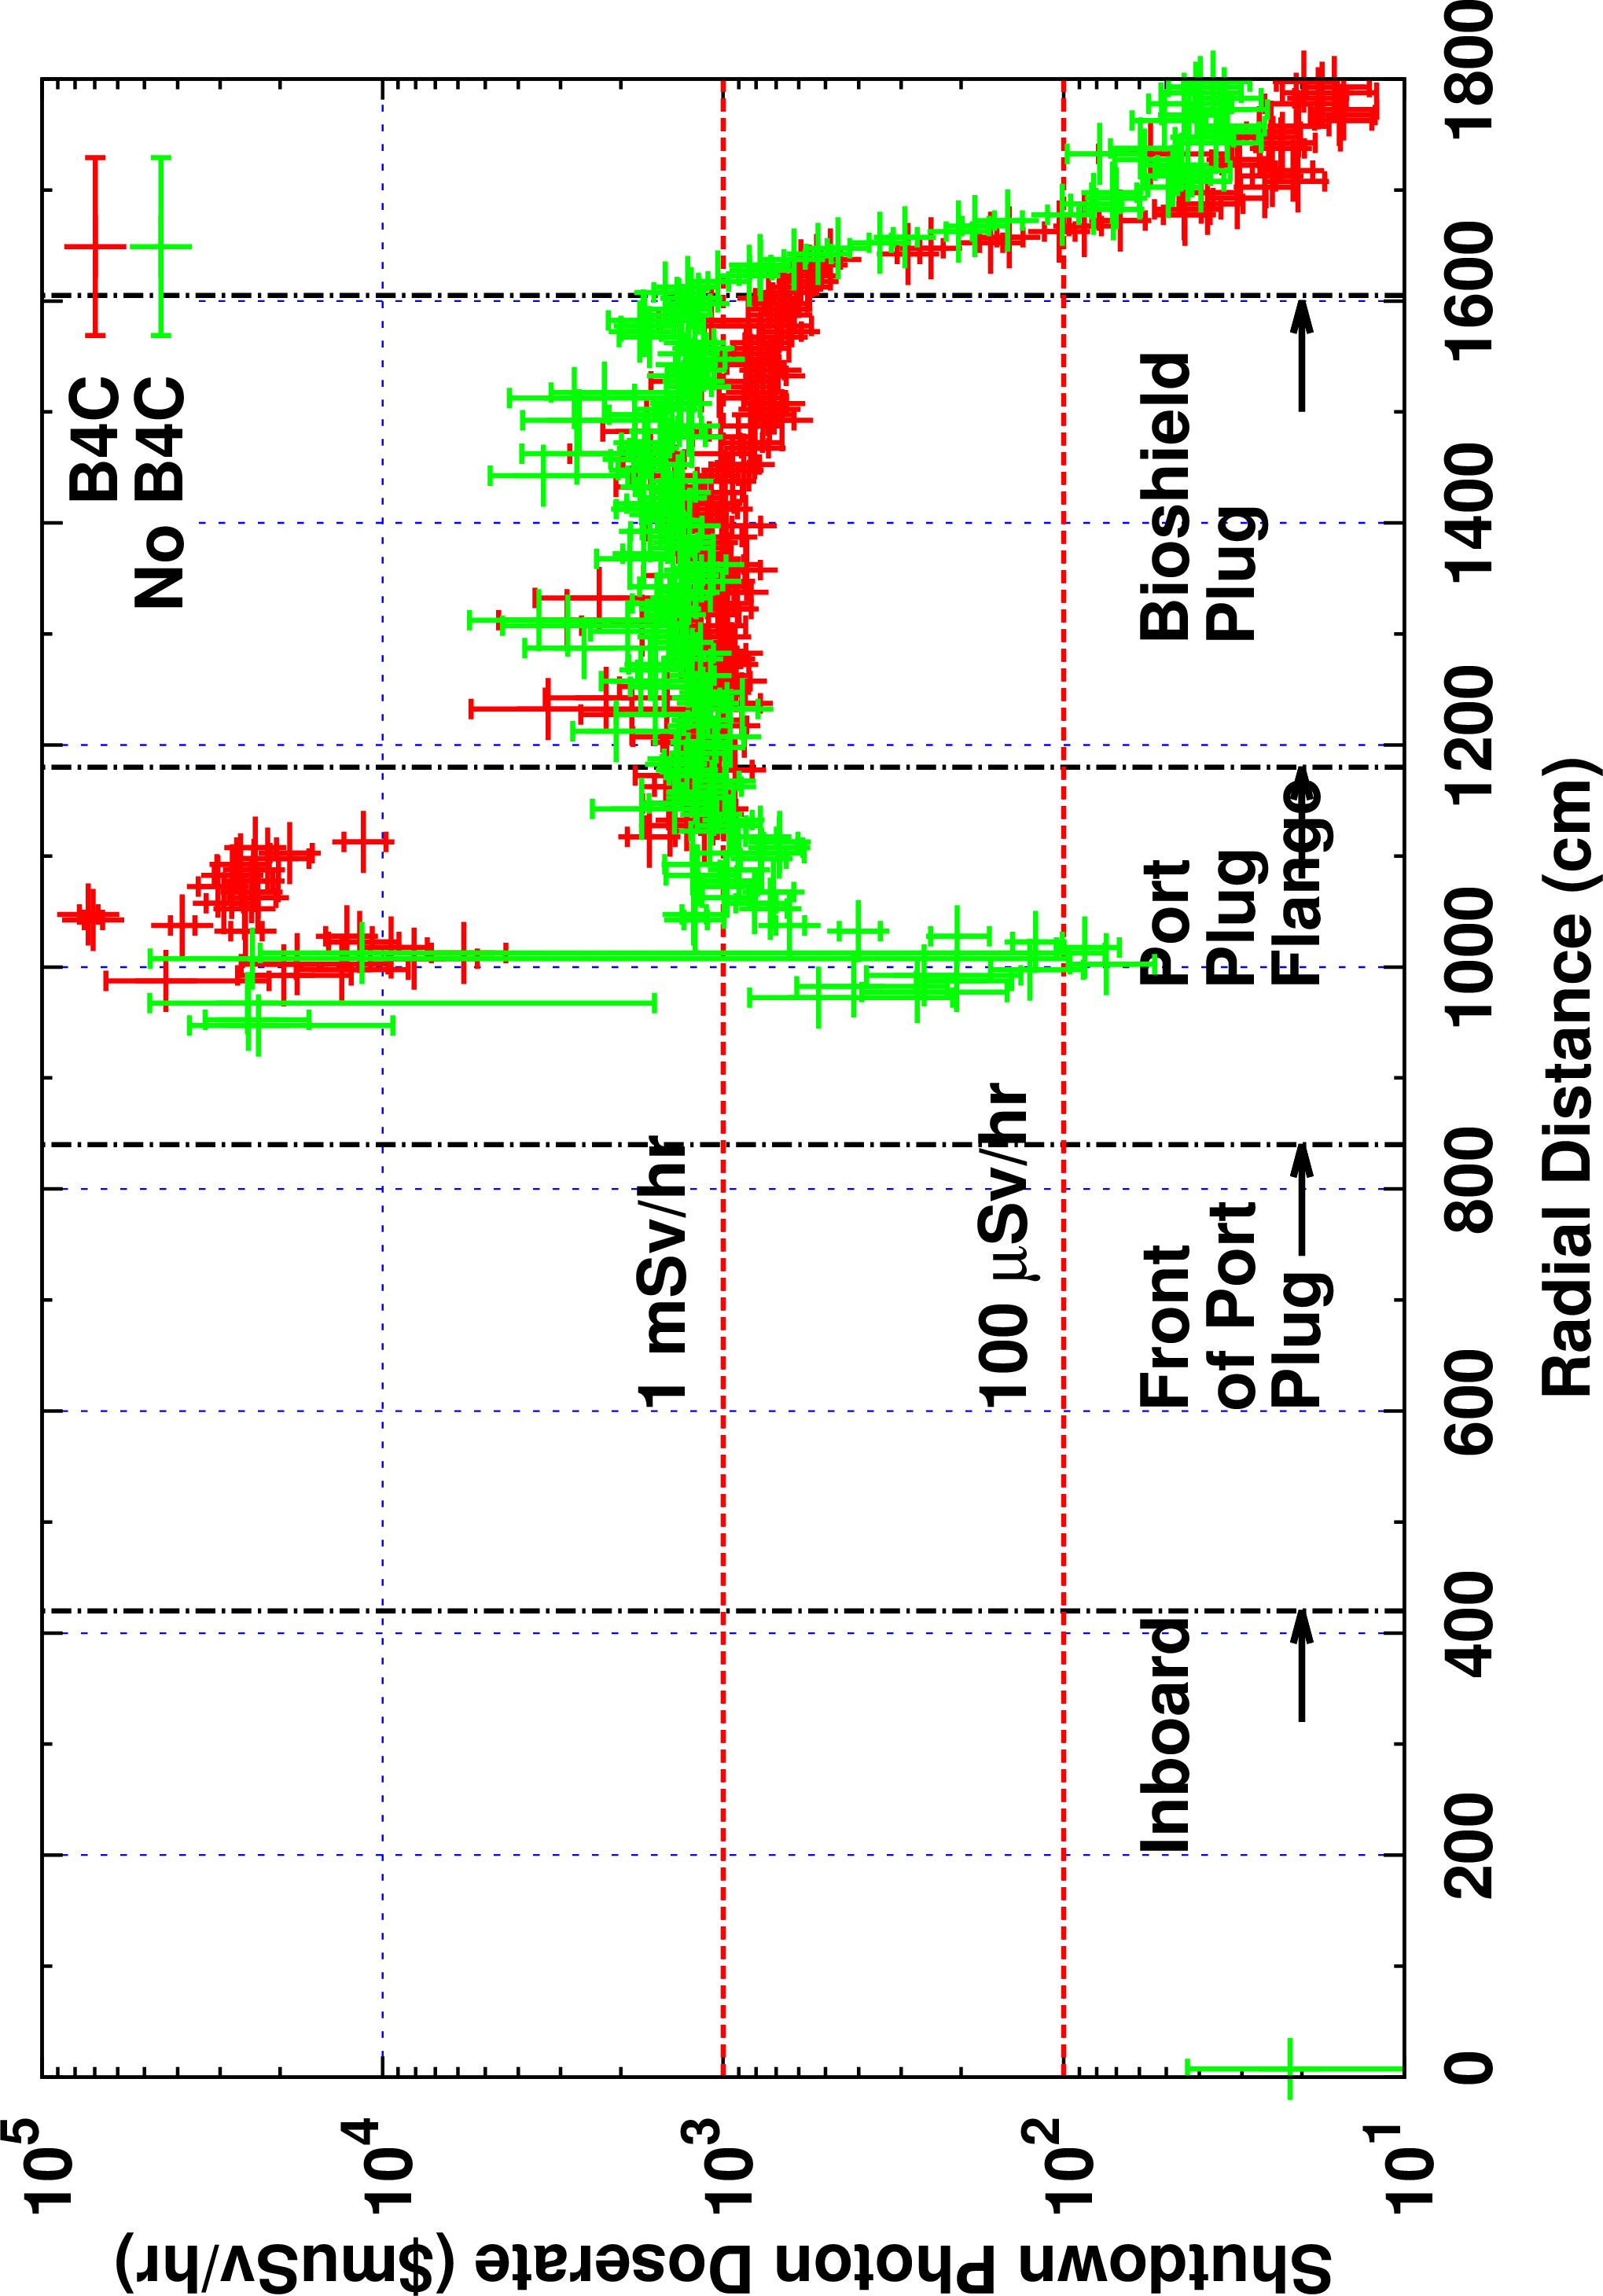
\includegraphics[clip,scale=0.12,angle=-90]{../plots/photon_lineout/comp/5yr_dc1.png}
\caption{Total dose rate along a line from 0,0,60 to 1800,0,60 cm for the ``SA-2 - 10'' irradiation
for both the B$_4$C and No B$_4$C case at $10^5$ s}
\label{fig:photons_5y_dc1_dose}
\end{figure}
\begin{figure}[ht!]
\centering
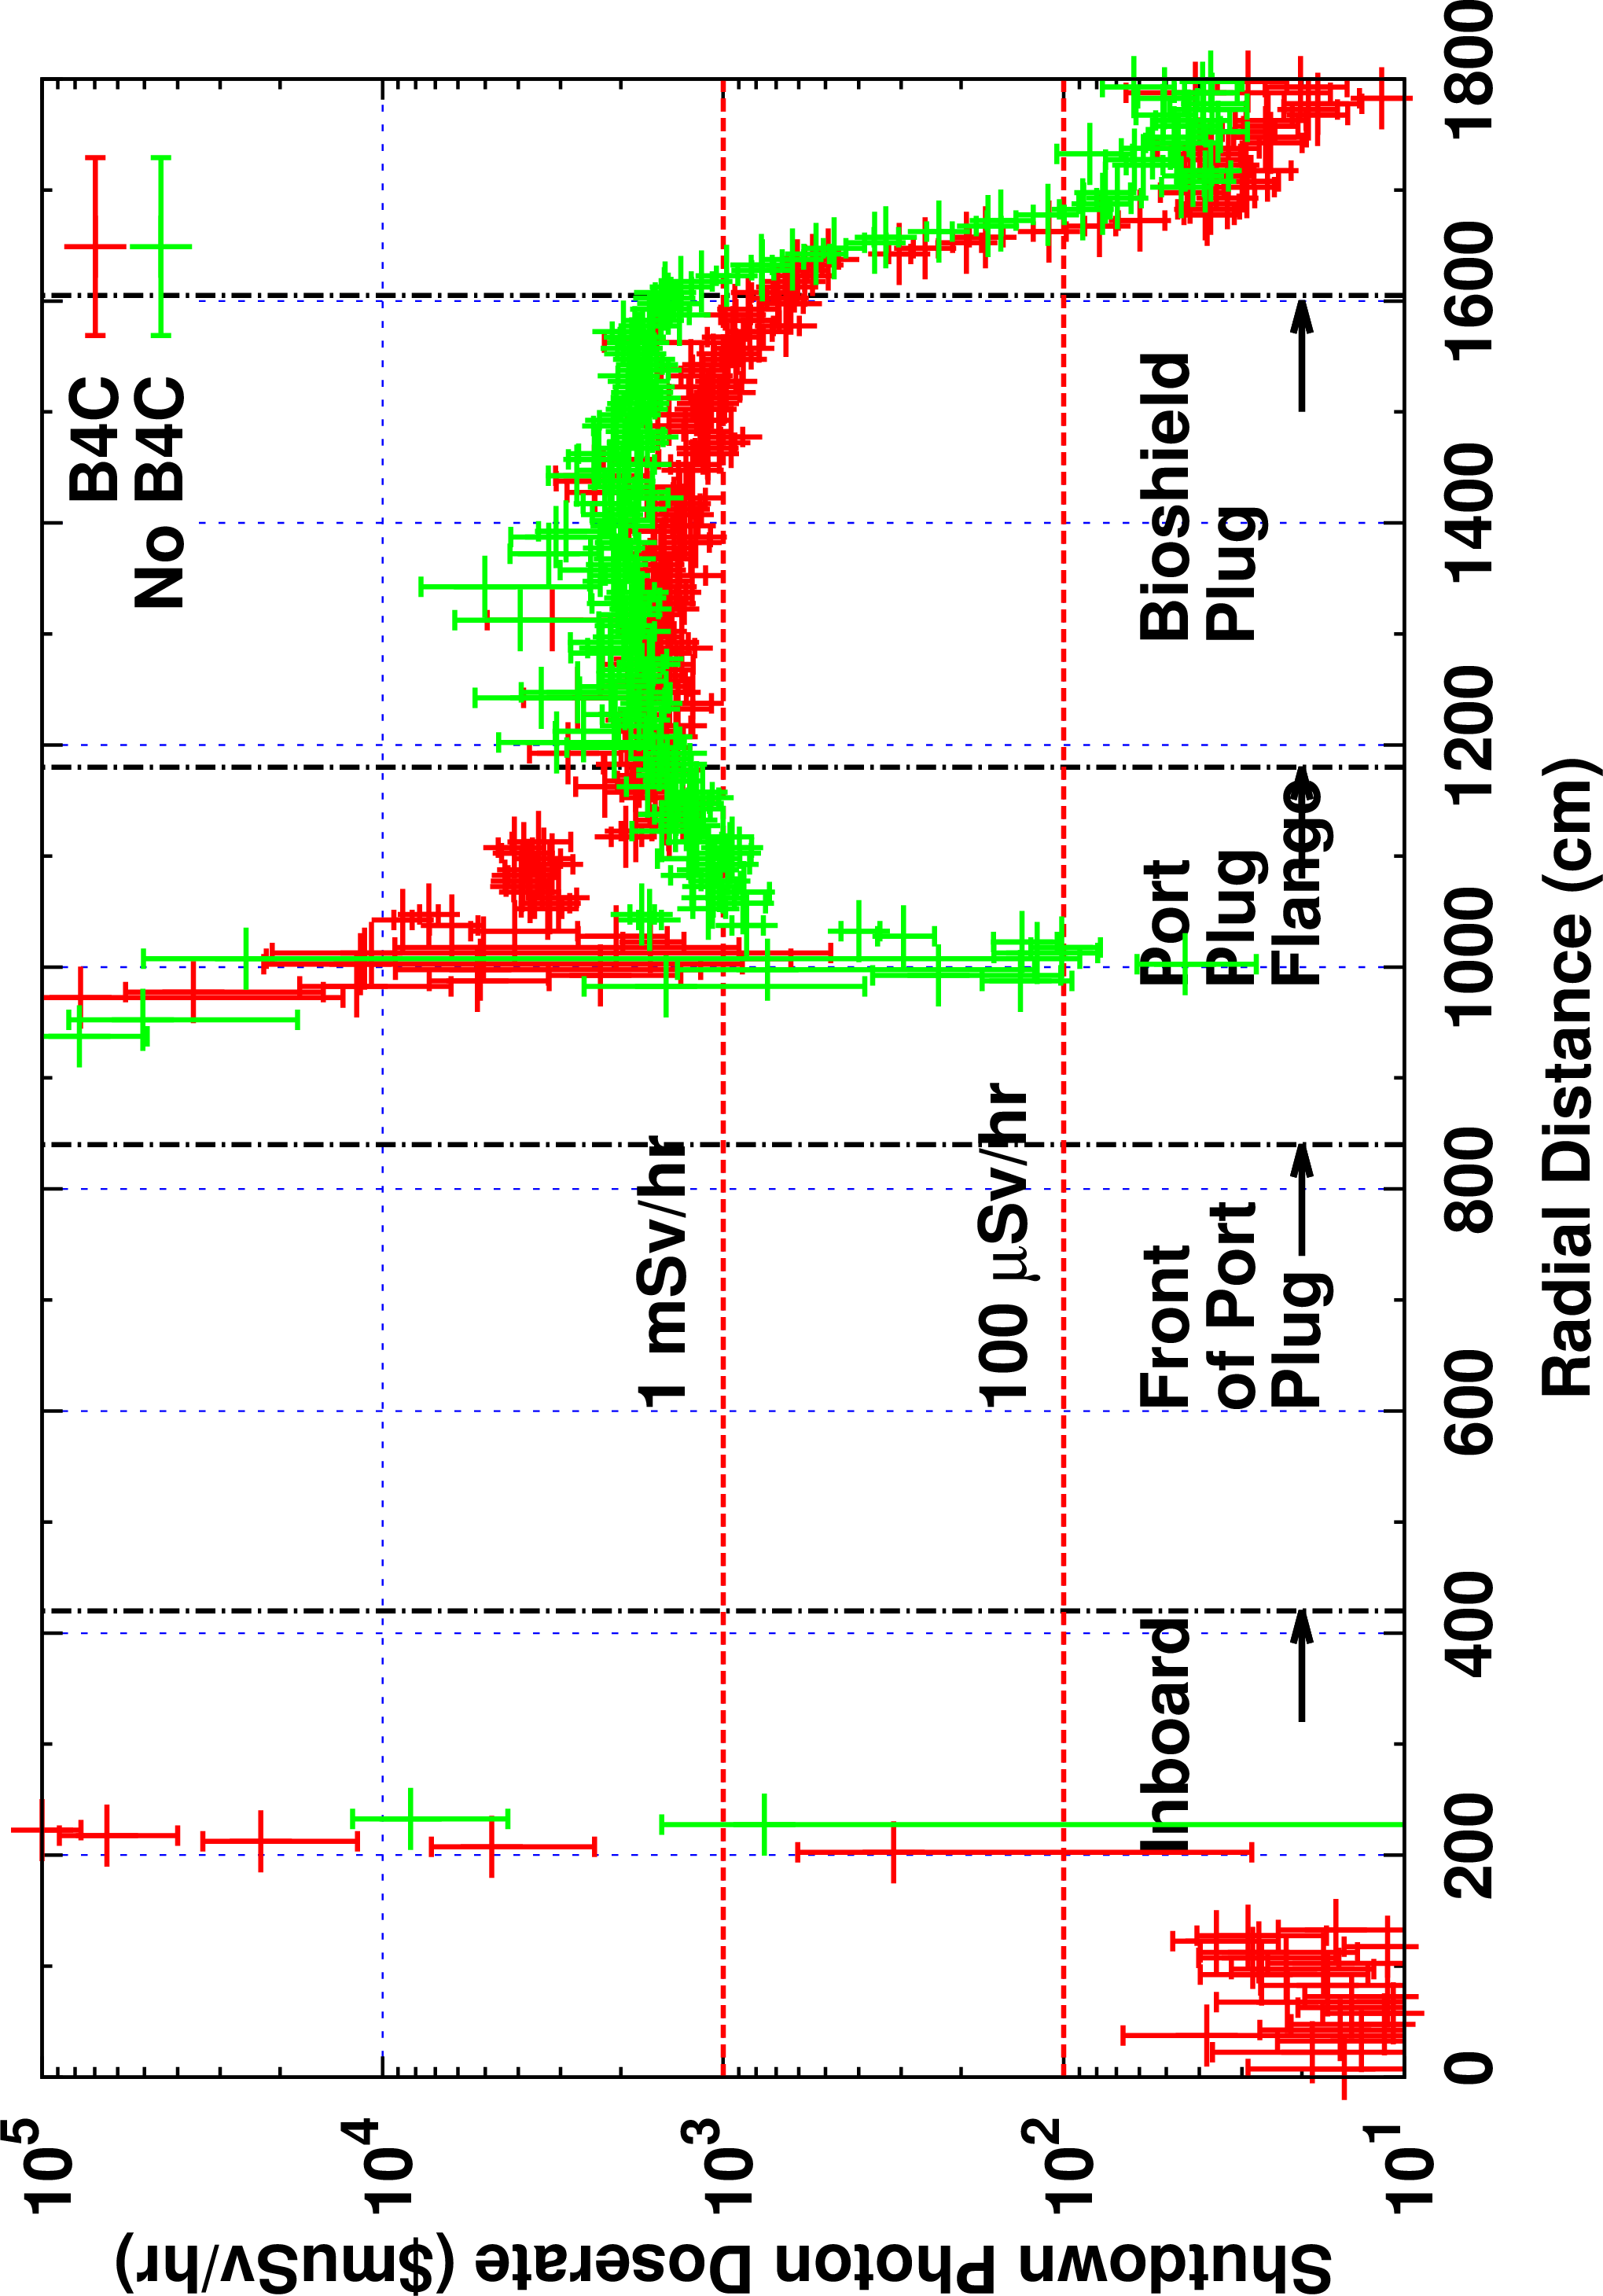
\includegraphics[clip,scale=0.12,angle=-90]{../plots/photon_lineout/comp/10yr_dc1.png}
\caption{Total dose rate along a line from 0,0,60 to 1800,0,60 cm for the ``SA-2 - 5'' irradiation
for both the B$_4$C and No B$_4$C case at $10^5$ s}
\label{fig:photons_10y_dc1_dose}
\end{figure}
\newpage
\subsubsection{Decay Time 2 - 1$\times$10$^{6}$ s}
\begin{figure}[ht!]
\centering
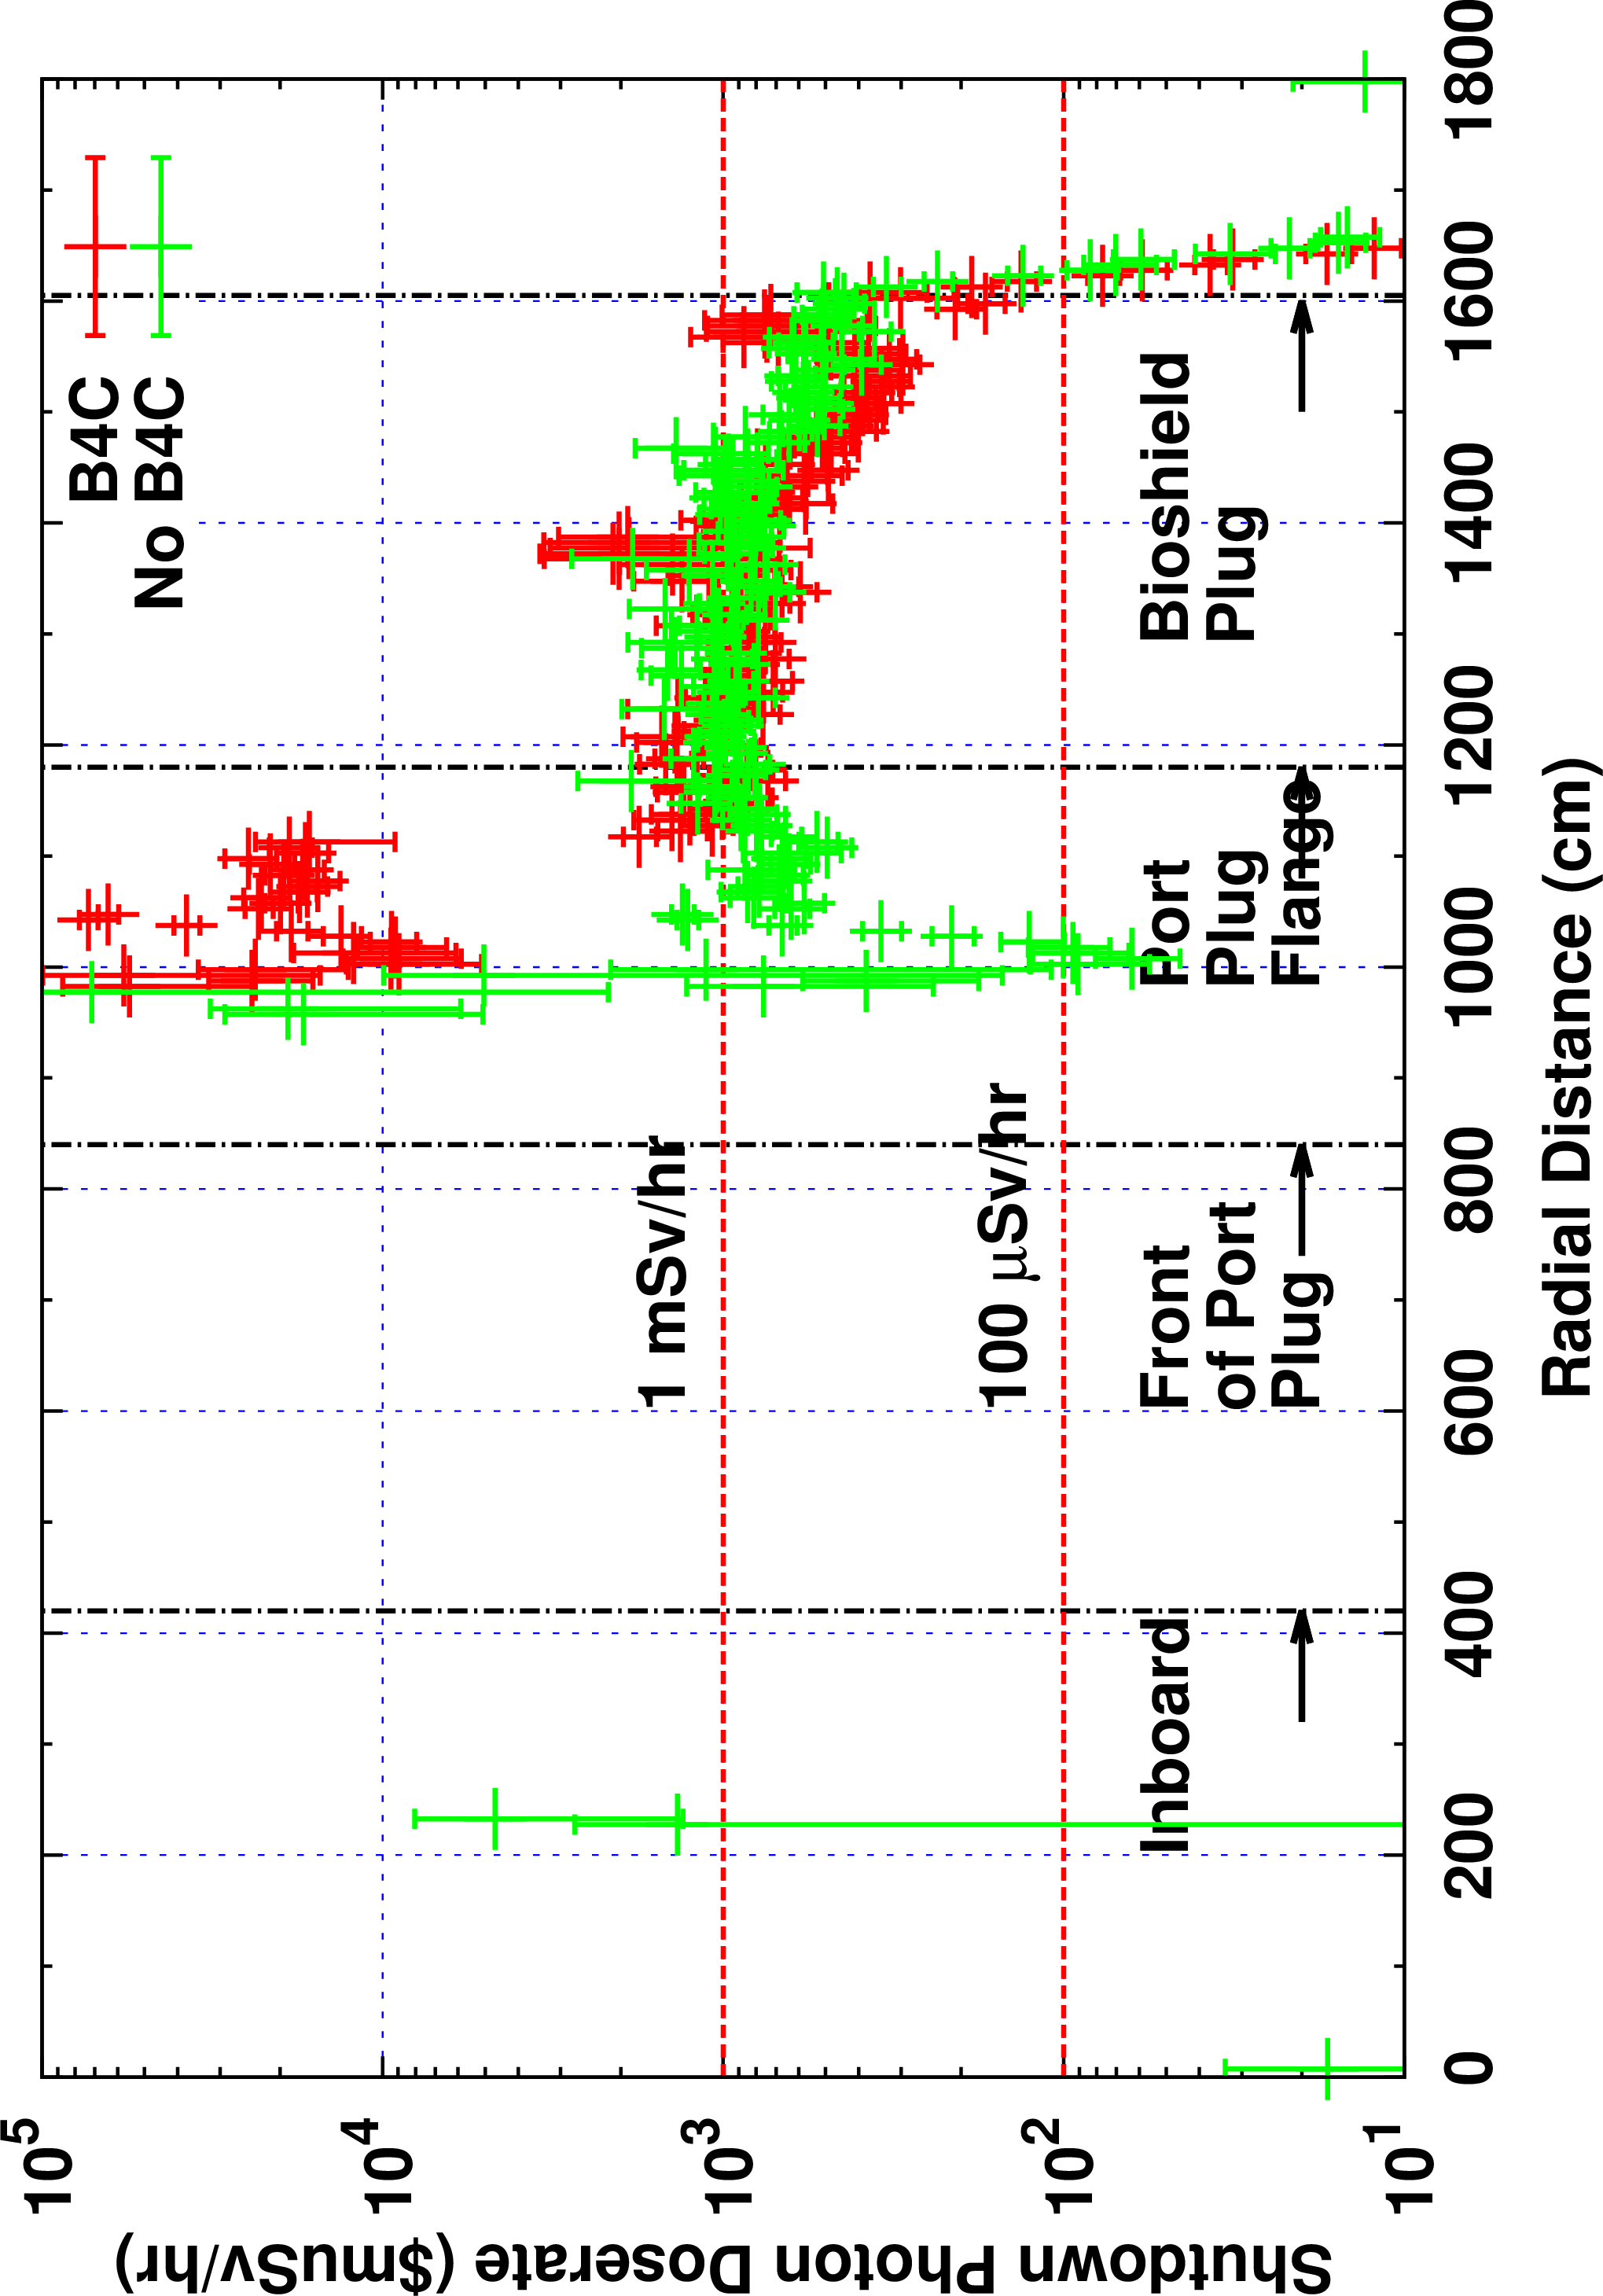
\includegraphics[clip,scale=0.12,angle=-90]{../plots/photon_lineout/comp/5yr_dc2.png}
\caption{Total dose rate along a line from 0,0,60 to 1800,0,60 cm for the ``SA-2 - 10'' irradiation
for both the B$_4$C and No B$_4$C case at $10^6$ s}
\label{fig:photons_5y_dc2_dose}
\end{figure}
\begin{figure}[ht!]
\centering
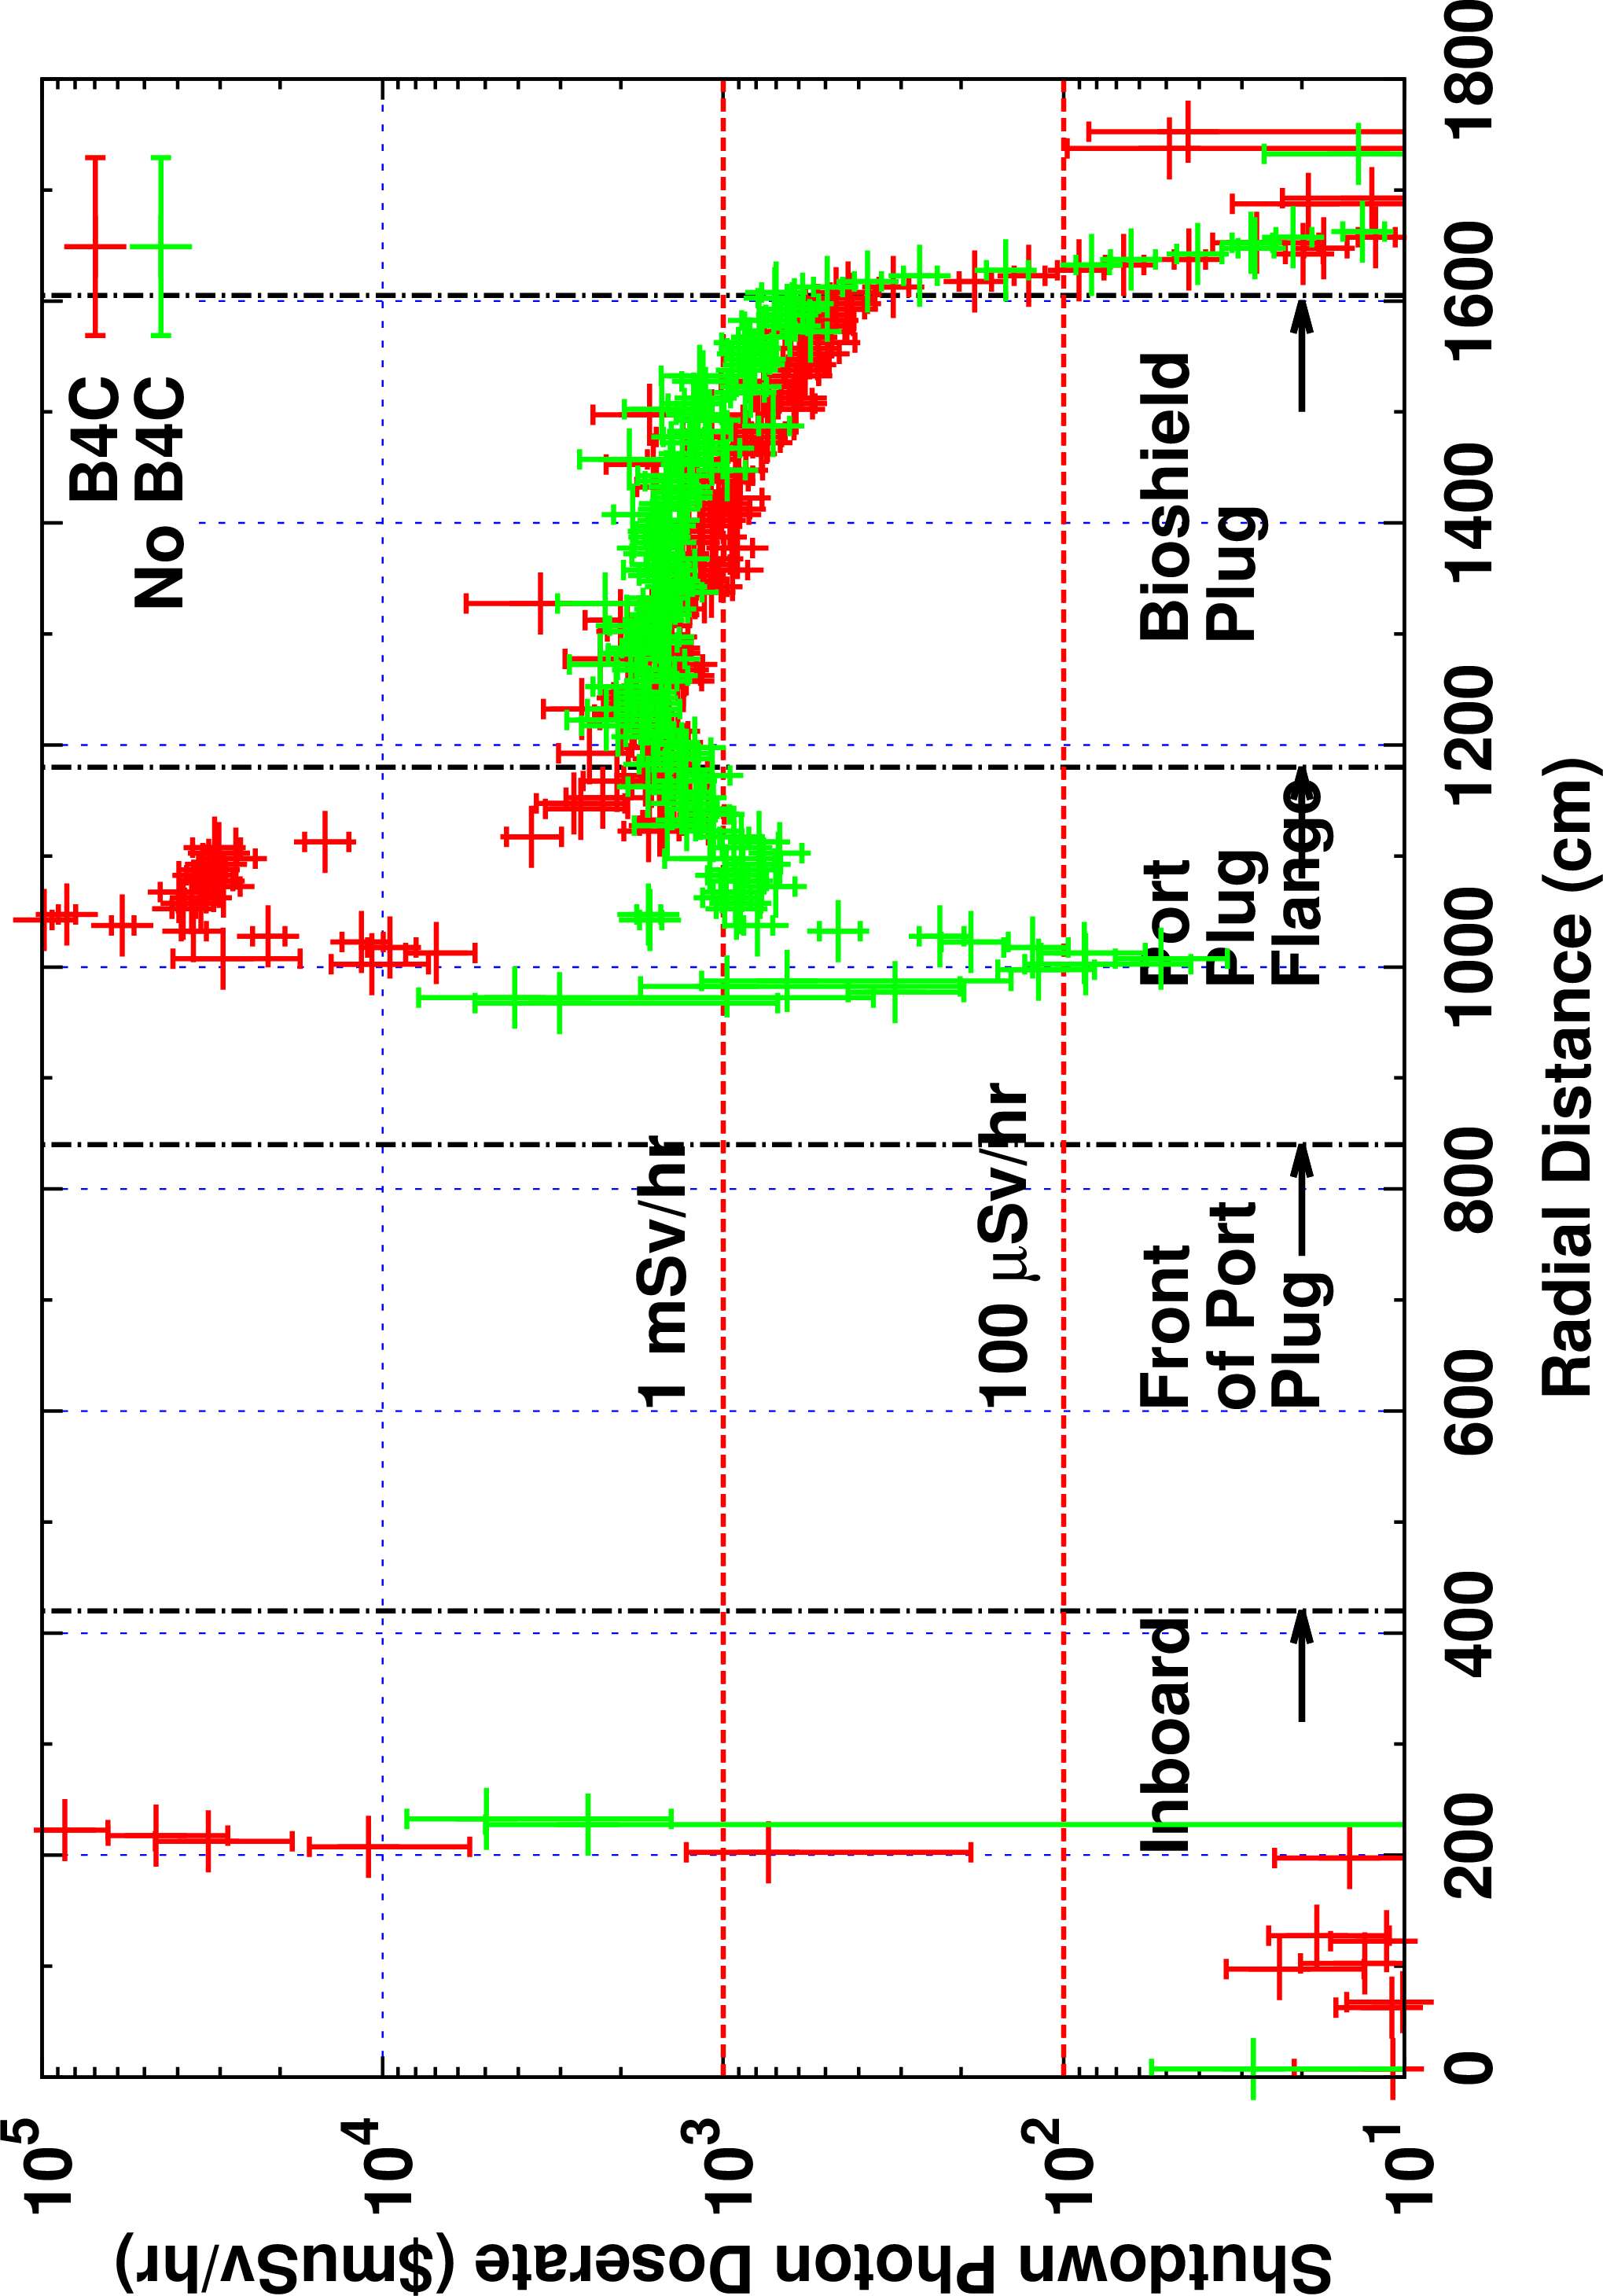
\includegraphics[clip,scale=0.12,angle=-90]{../plots/photon_lineout/comp/10yr_dc2.png}
\caption{Total dose rate along a line from 0,0,60 to 1800,0,60 cm for the ``SA-2 - 5'' irradiation
for both the B$_4$C and No B$_4$C case at $10^6$ s}
\label{fig:photons_10y_dc2_dose}
\end{figure}
\newpage
\subsubsection{Decay Time 3 - 1$\times$10$^{7}$ s}
\begin{figure}[ht!]
\centering
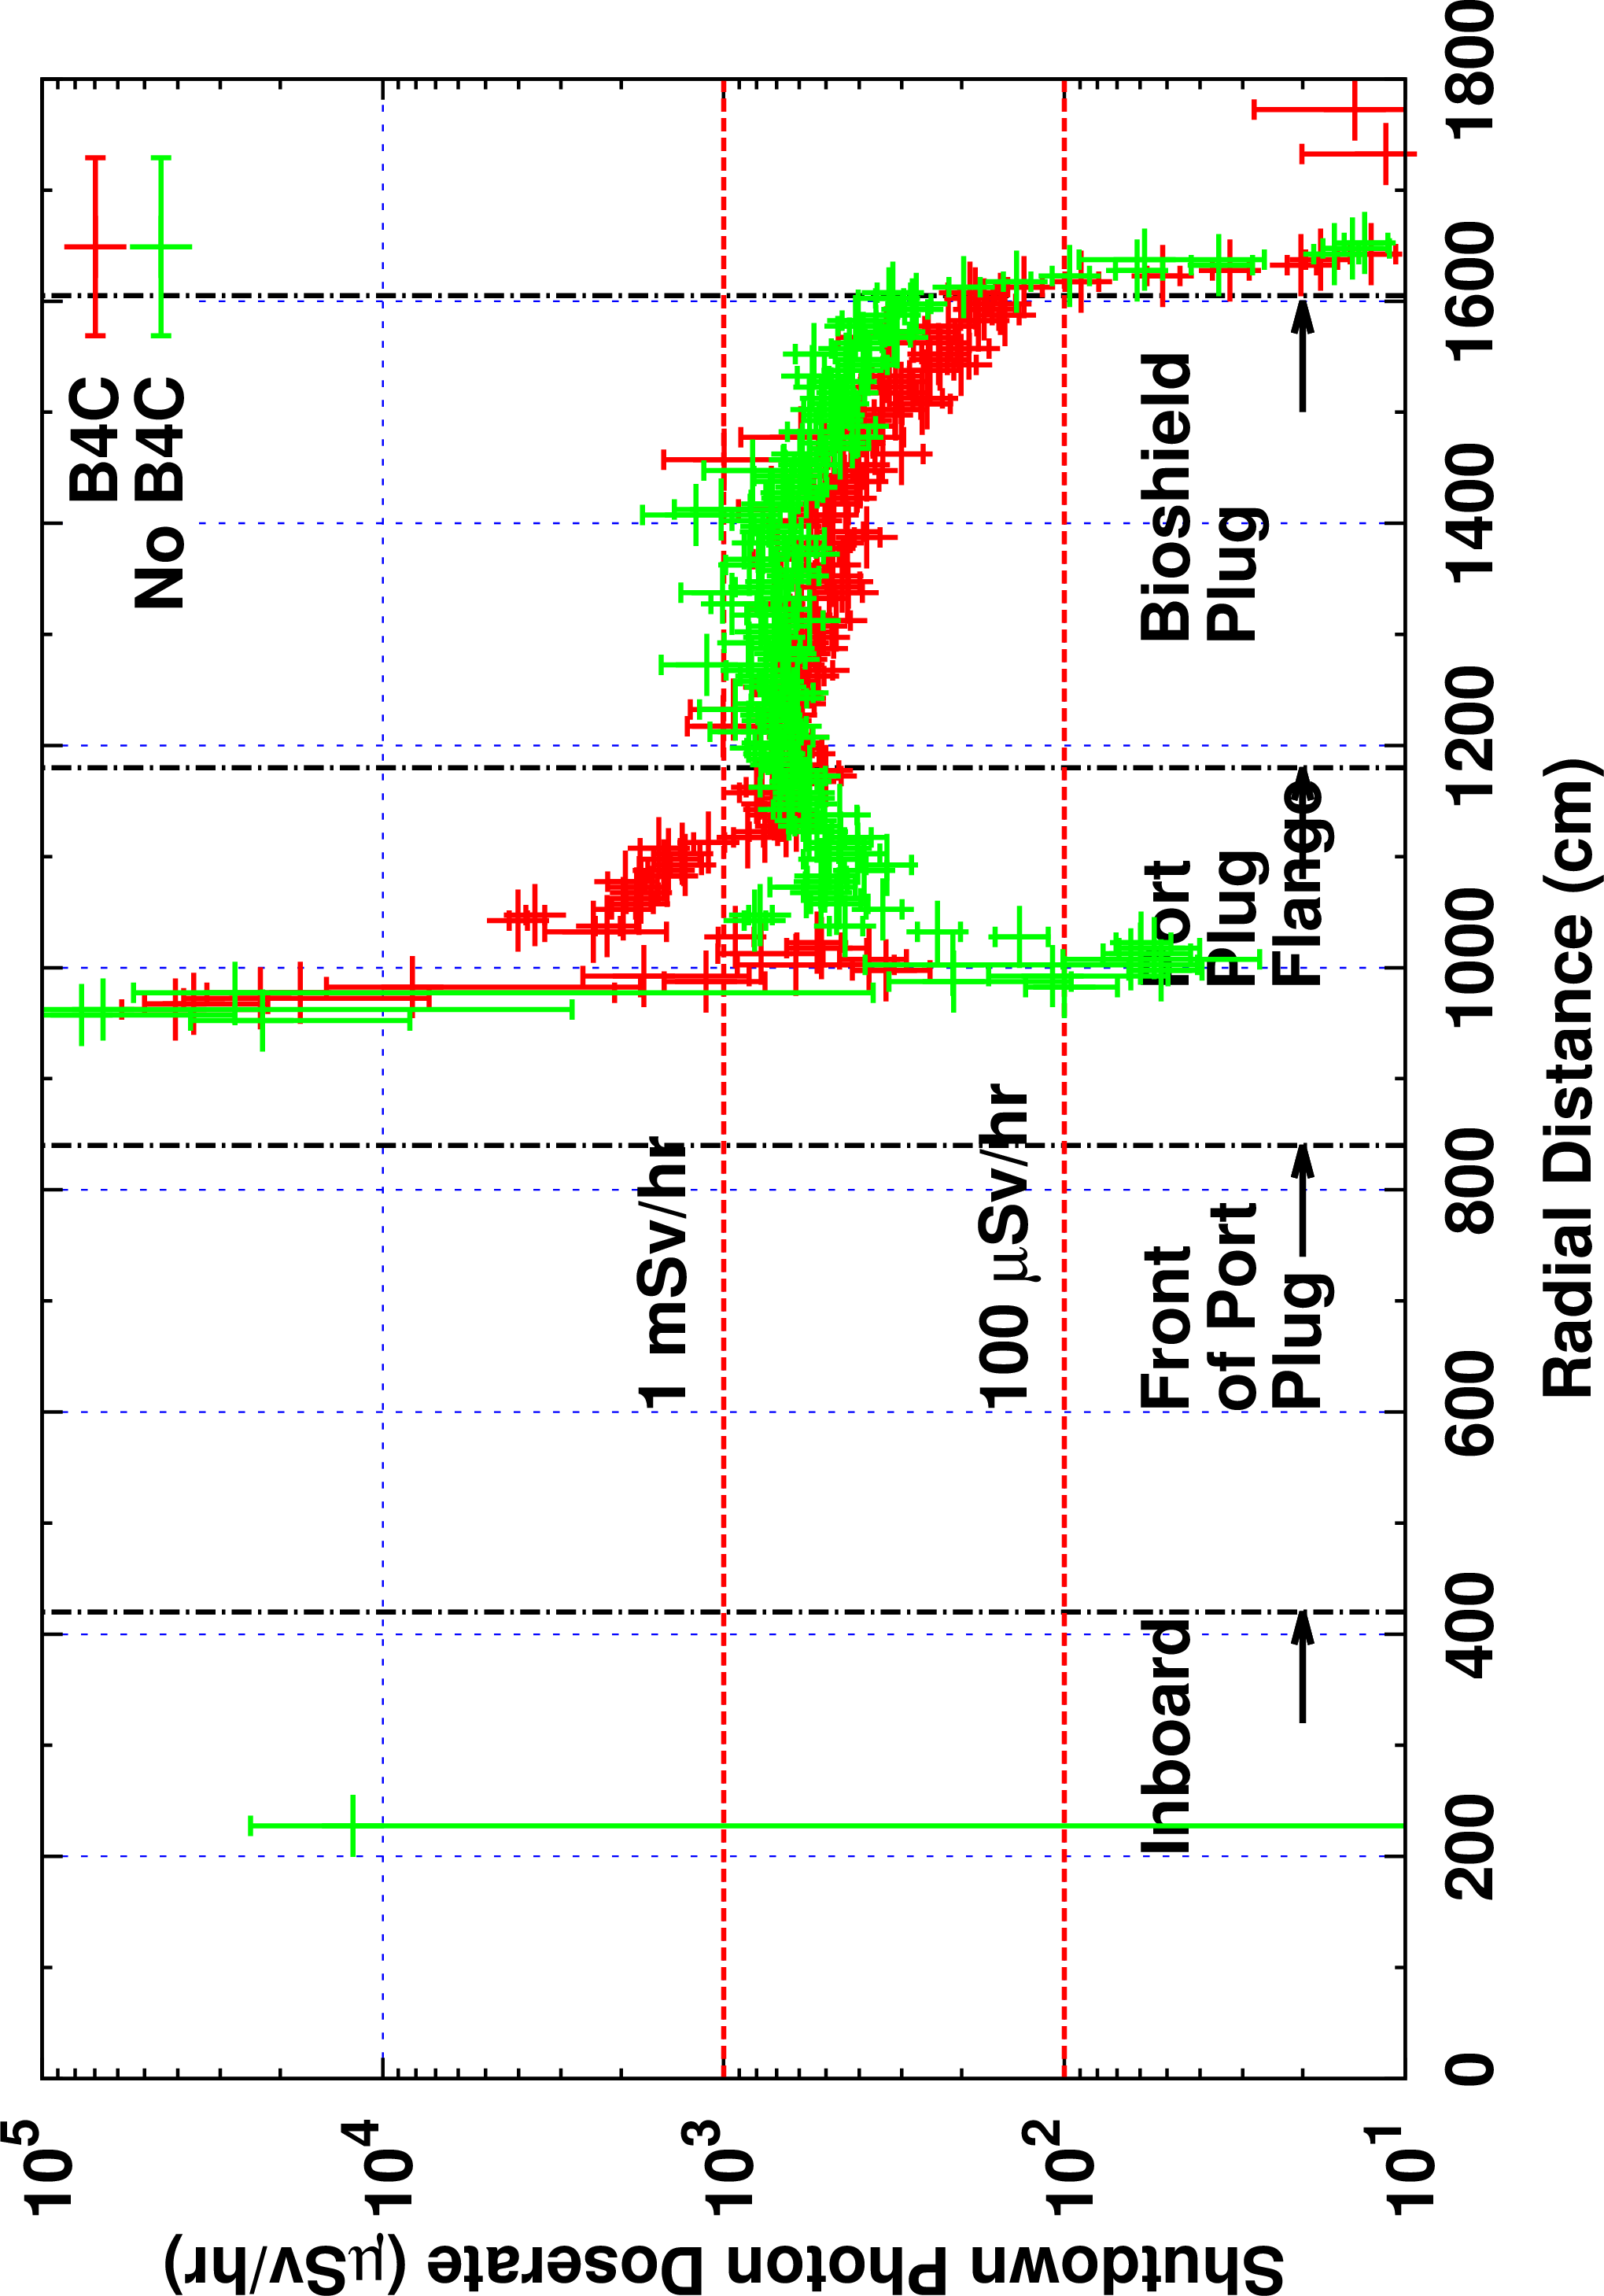
\includegraphics[clip,scale=0.12,angle=-90]{../plots/photon_lineout/comp/5yr_dc3.png}
\caption{Total dose rate along a line from 0,0,60 to 1800,0,60 cm for the ``SA-2 - 10'' irradiation
for both the B$_4$C and No B$_4$C case at $10^7$ s}
\label{fig:photons_5y_dc3_dose}
\end{figure}
\begin{figure}[ht!]
\centering
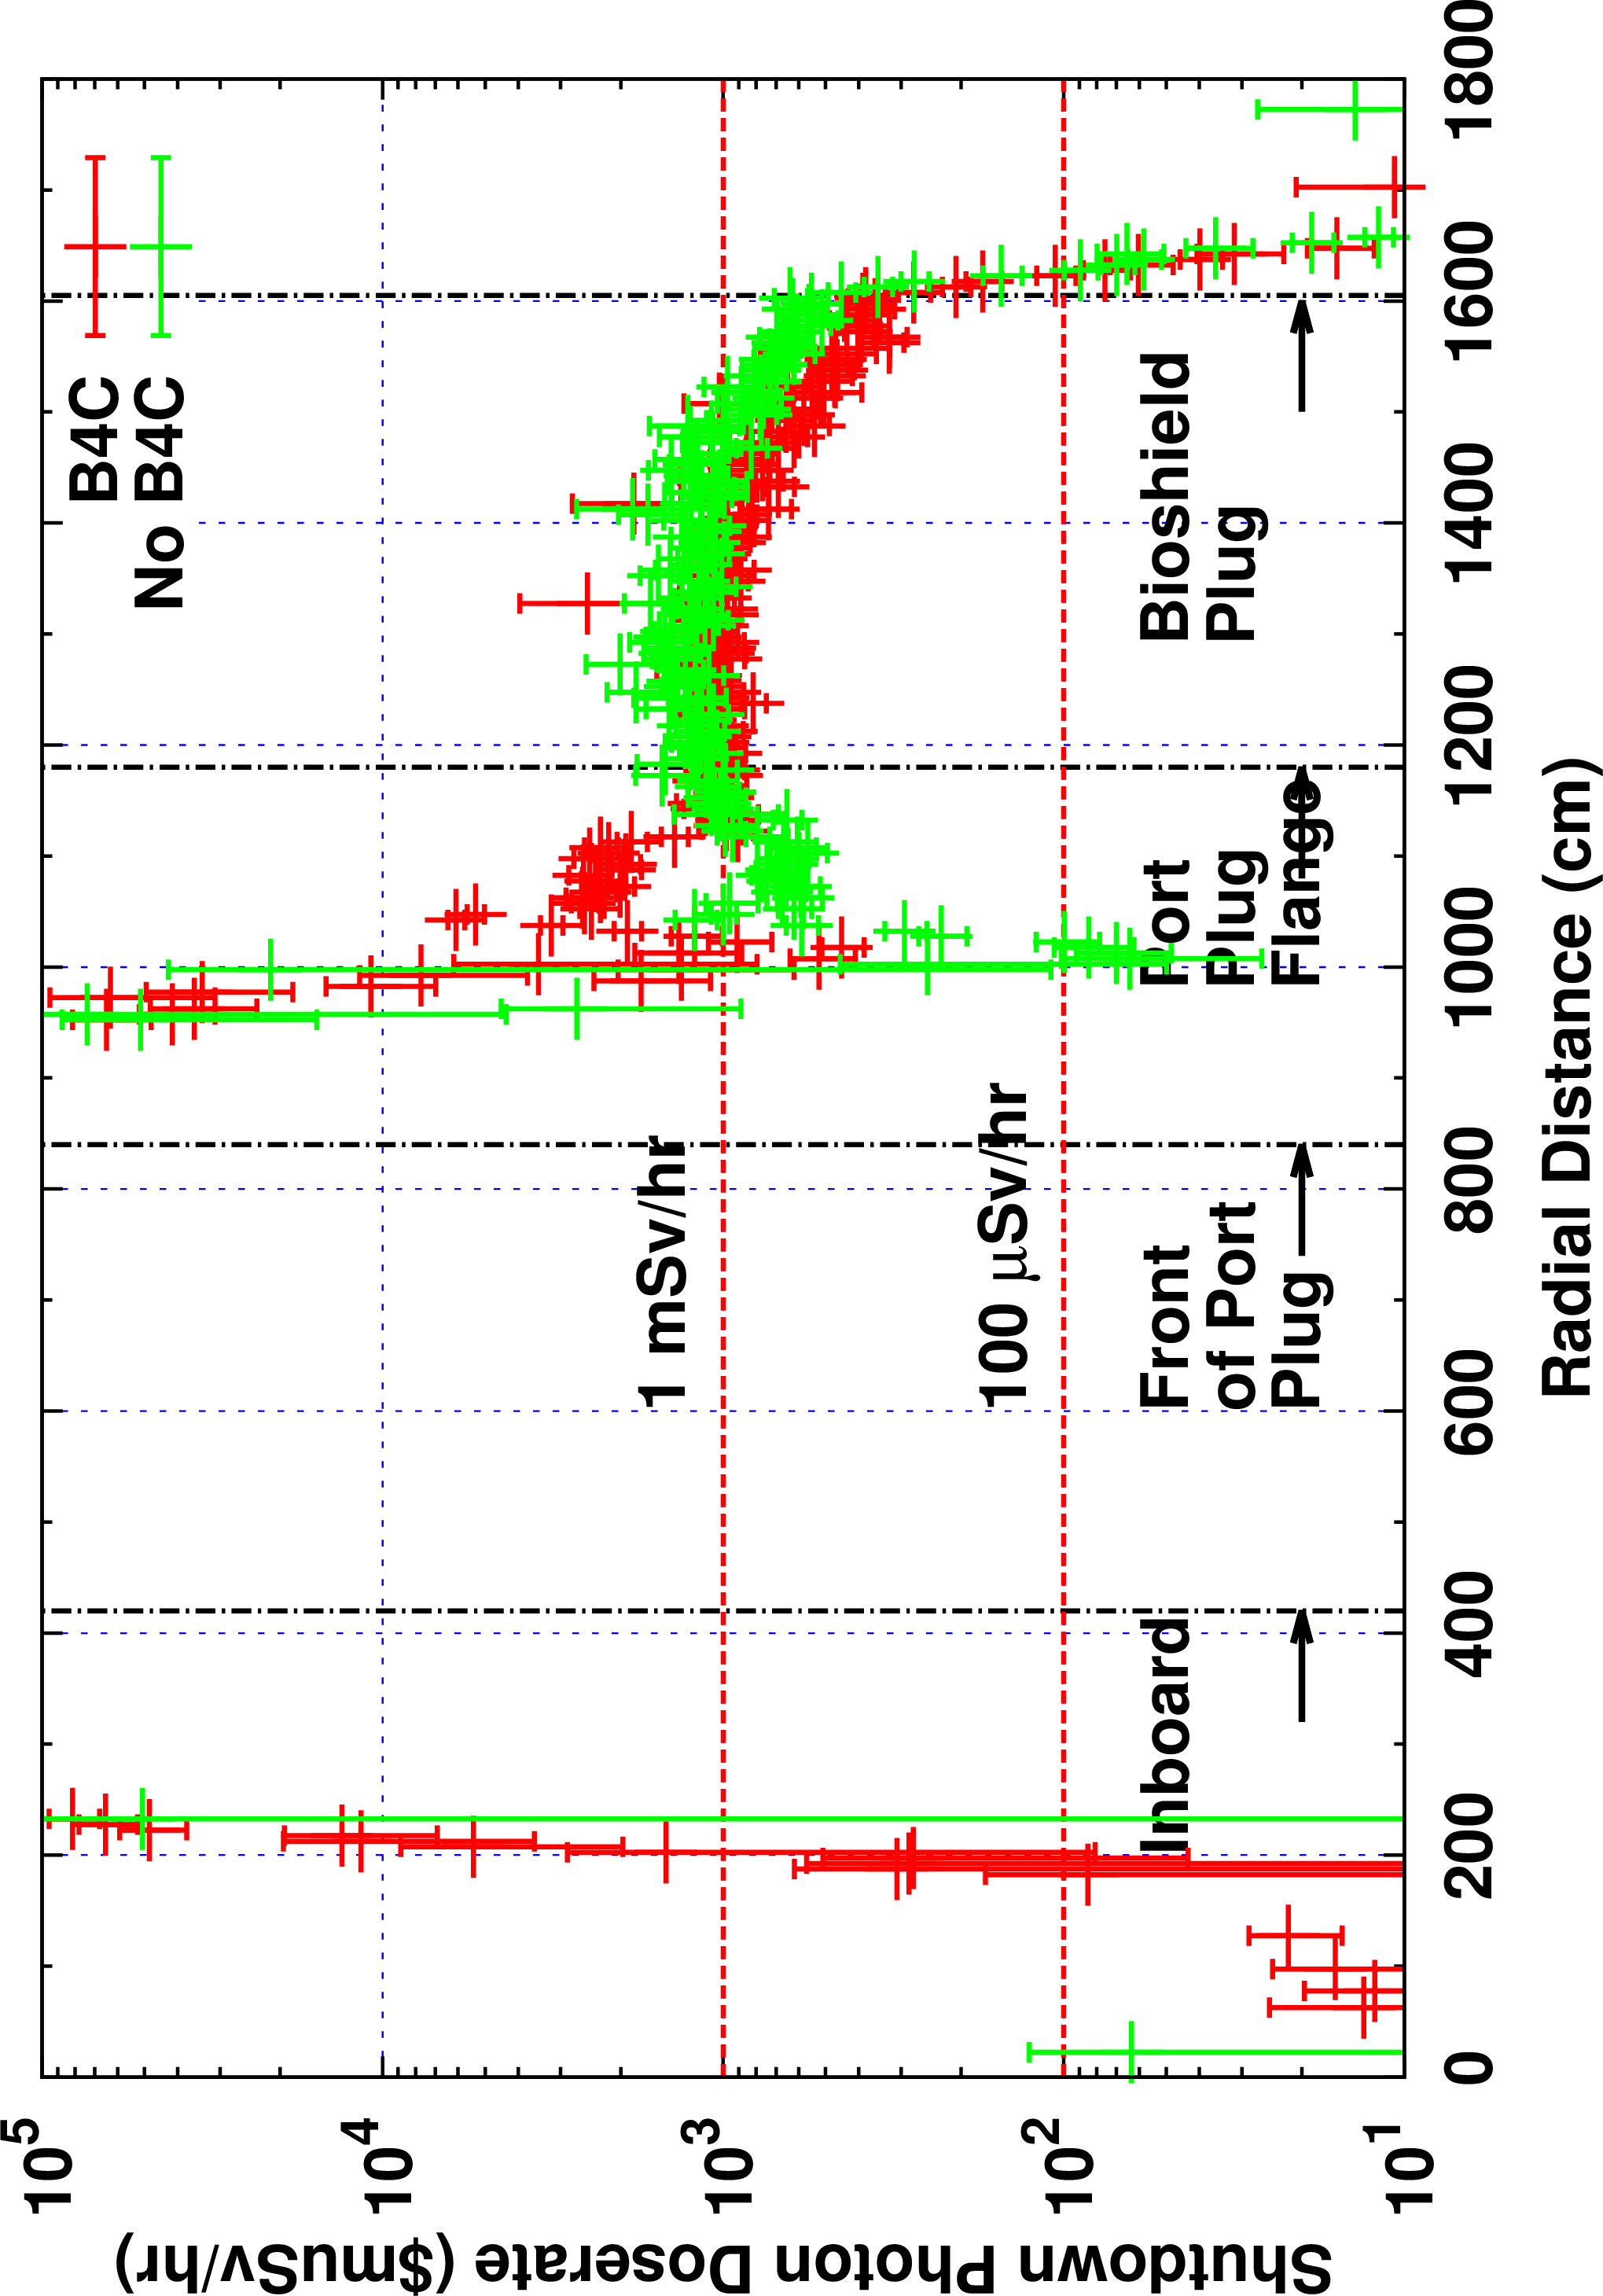
\includegraphics[clip,scale=0.12,angle=-90]{../plots/photon_lineout/comp/10yr_dc3.png}
\caption{Total dose rate along a line from 0,0,60 to 1800,0,60 cm for the ``SA-2 - 5'' irradiation
for both the B$_4$C and No B$_4$C case at $10^7$ s}
\label{fig:photons_10y_dc3_dose}
\end{figure}
\clearpage
\newpage
\subsection{Summary}
\subsubsection*{B$_4$C}
As shown in Section \ref{sec:sdr_results_b4c} most points within equatorial port
interspace are below 1 mSv/hr for the ``SA-2 - 10'' irradiation. For the ``SA-2 - 5''
irradiation however, the majority of points across all decay times are
greater than 1 mSv/hr with the exception of points at positions greater than
1400 cm where reductions below 1 mSv/hr can be seen.
\subsubsection*{No B$_4$C}
Of note is that for the ``SA-2 - 5'' irradiation and for all decay 
times most points in the equatorial port interspace are above 1 mSv/hr. However,
for the ``SA-2 - 10'' irradiation we see that by the second decay time most points 
are under 1 mSv/hr, but are still in excess of 100 $\mu$Sv/hr. 
\subsubsection*{Comparison}
The immediate differences between the B$_4$C and no B$_4$C are the same as in 
the full report, in the port interspace the SDR is lower adjacent to the 
bioshield for all cases across all decay times. There are some cases where
just behind the equatorial port plug flange the dose can be higher in the 
B$_4$C than in the no B$_4$C case, this is likely due to a large error in the 
activation source there due to a poor estimate of the neutron flux. 
\clearpage
\newpage
\section{Conclusion}
A set of sequence of neutron activation calculations were performed for a suite 
of 3 different irradiation scenarios. The ITER SA-2 scenario that has a
fluence of 266.5 MWy, the ``SA-2 - 5 year'' scenario with a fluence of 163.5 MWy and
the ``SA-2 - 10 year'' scenario with a fluence of 60.5 MWy. A brief summary of
results chosen at a point on the external surface of the bioshield plug are shown in
shown in Tables \ref{tab:b4c_summary_scenario} and \ref{tab:nob4c_summary_scenario}.

\begin{table}[ht!]
   \centering      
   \begin{tabular}{| c | c | c | c |}
      \hline
      & SA2 & ``SA-2 - 5 Yr'' & ``SA-2 - 10 Yr'' \\
      \hline
      Decay Time (s) & Dose Rate & Dose Rate & Dose Rate \\
      \hline
      1.0$\times$10$^{5}$ & 1.053$\times$10$^{3}$ $\pm$ 6.42\% & 6.813$\times$10$^{2}$ $\pm$ 7.82\% & 5.582$\times$10$^{2}$ $\pm$ 7.47\%\\
      1.0$\times$10$^{6}$ & 4.182$\times$10$^{2}$ $\pm$ 16.2\% & 4.206$\times$10$^{2}$ $\pm$ 14.8\% & 1.857$\times$10$^{2}$ $\pm$ 23.4\%\\
      1.0$\times$10$^{7}$ & 3.685$\times$10$^{2}$ $\pm$ 12.4\% & 2.740$\times$10$^{2}$ $\pm$ 11.3\% & 1.527$\times$10$^{2}$ $\pm$ 16.8\%\\
      \hline
\end{tabular}
\caption{B4C Results - Considering a point at the external surface of the bioshield plug}
\label{tab:b4c_summary_scenario}
\end{table}

\begin{table}[ht!]
   \centering      
   \begin{tabular}{| c | c | c | c |}
      \hline
      & SA2 & ``SA-2 - 5 Yr'' & ``SA-2 - 10 Yr'' \\
      \hline
      Decay Time (s) & Dose Rate & Dose Rate & Dose Rate \\
      \hline
      1.0$\times$10$^{5}$ & 2.509$\times$10$^{3}$ $\pm$ 8.37\% & 1.351$\times$10$^{3}$ $\pm$ 6.52\% & 1.133$\times$10$^{3}$ $\pm$ 6.3\%\\
      1.0$\times$10$^{6}$ & 6.241$\times$10$^{2}$ $\pm$ 11.6\% & 4.430$\times$10$^{2}$ $\pm$ 11.4\% & 2.628$\times$10$^{2}$ $\pm$ 11.0\%\\
      1.0$\times$10$^{7}$ & 7.277$\times$10$^{2}$ $\pm$ 13.4\% & 4.024$\times$10$^{2}$ $\pm$ 11.7\% & 2.806$\times$10$^{2}$ $\pm$ 11.7\%\\
      \hline
\end{tabular}
\caption{No B4C Results - Considering a point at the external surface of the bioshield plug}
\label{tab:nob4c_summary_scenario}
\end{table}

The SDR results for the shortened irradiation times show the expected behavior 
that shorter irradiation times lead to lower accumulated activities and therefore
lower SDR.  There is also consistent behavior regarding the B$_4$C and no B$_4$C
cases for each decay time, where the B$_4$C is consistently the lower of the two.
\\
\\
These calculations show that even for reduced ITER operations times the SDR
in key maintenance areas are still above 100 $\mu$Sv/hr. 
\newpage
\bibliographystyle{unsrt}
\bibliography{bibliography}
\newpage
\clearpage
\section{Appendix A - B4C ``SA-2 - 10 Yr'' Irradiation }
\begin{figure}[ht!]
\centering
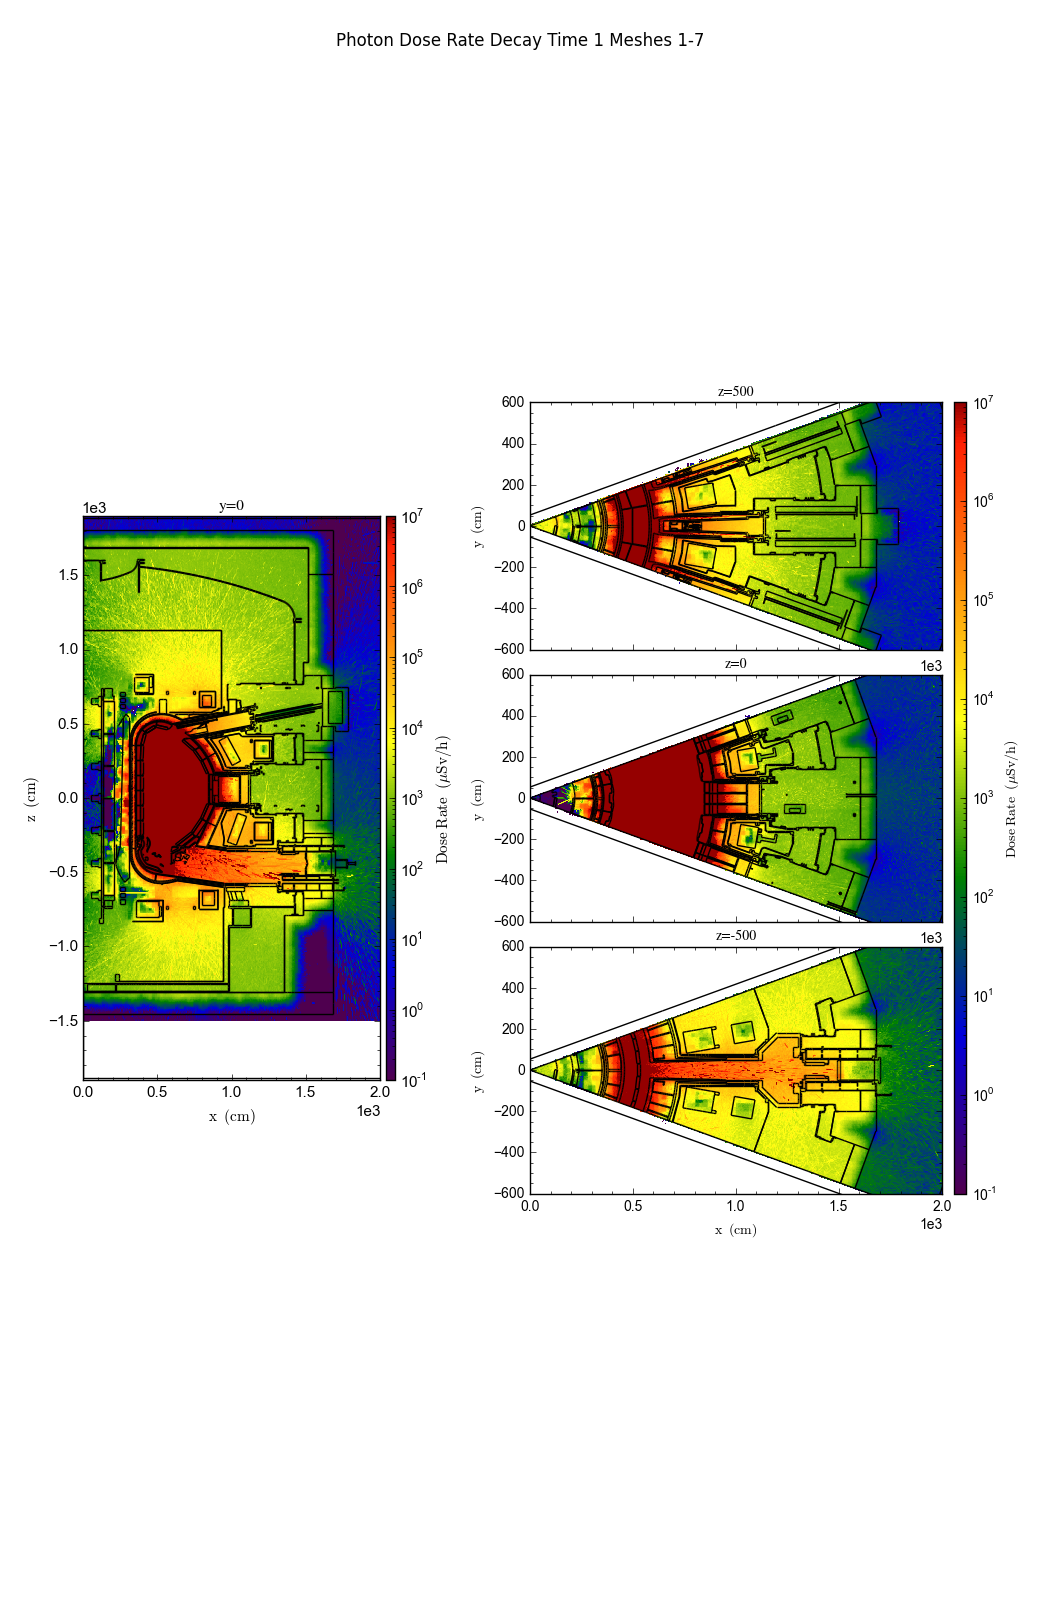
\includegraphics[trim={0cm 8cm, 0cm 8cm},clip,scale=0.75]{../plots/final_model_with_b4c/5year/Photon_Dose_Rate_Decay_Time_1_Meshes_1-7.png}
\caption{Total dose rate for decay time 1 for the ``SA-2 - 10 Yr'' irradiation}
\label{fig:photons_5y_dc1_b4c_dose}
\end{figure}
\begin{figure}[ht!]
\centering
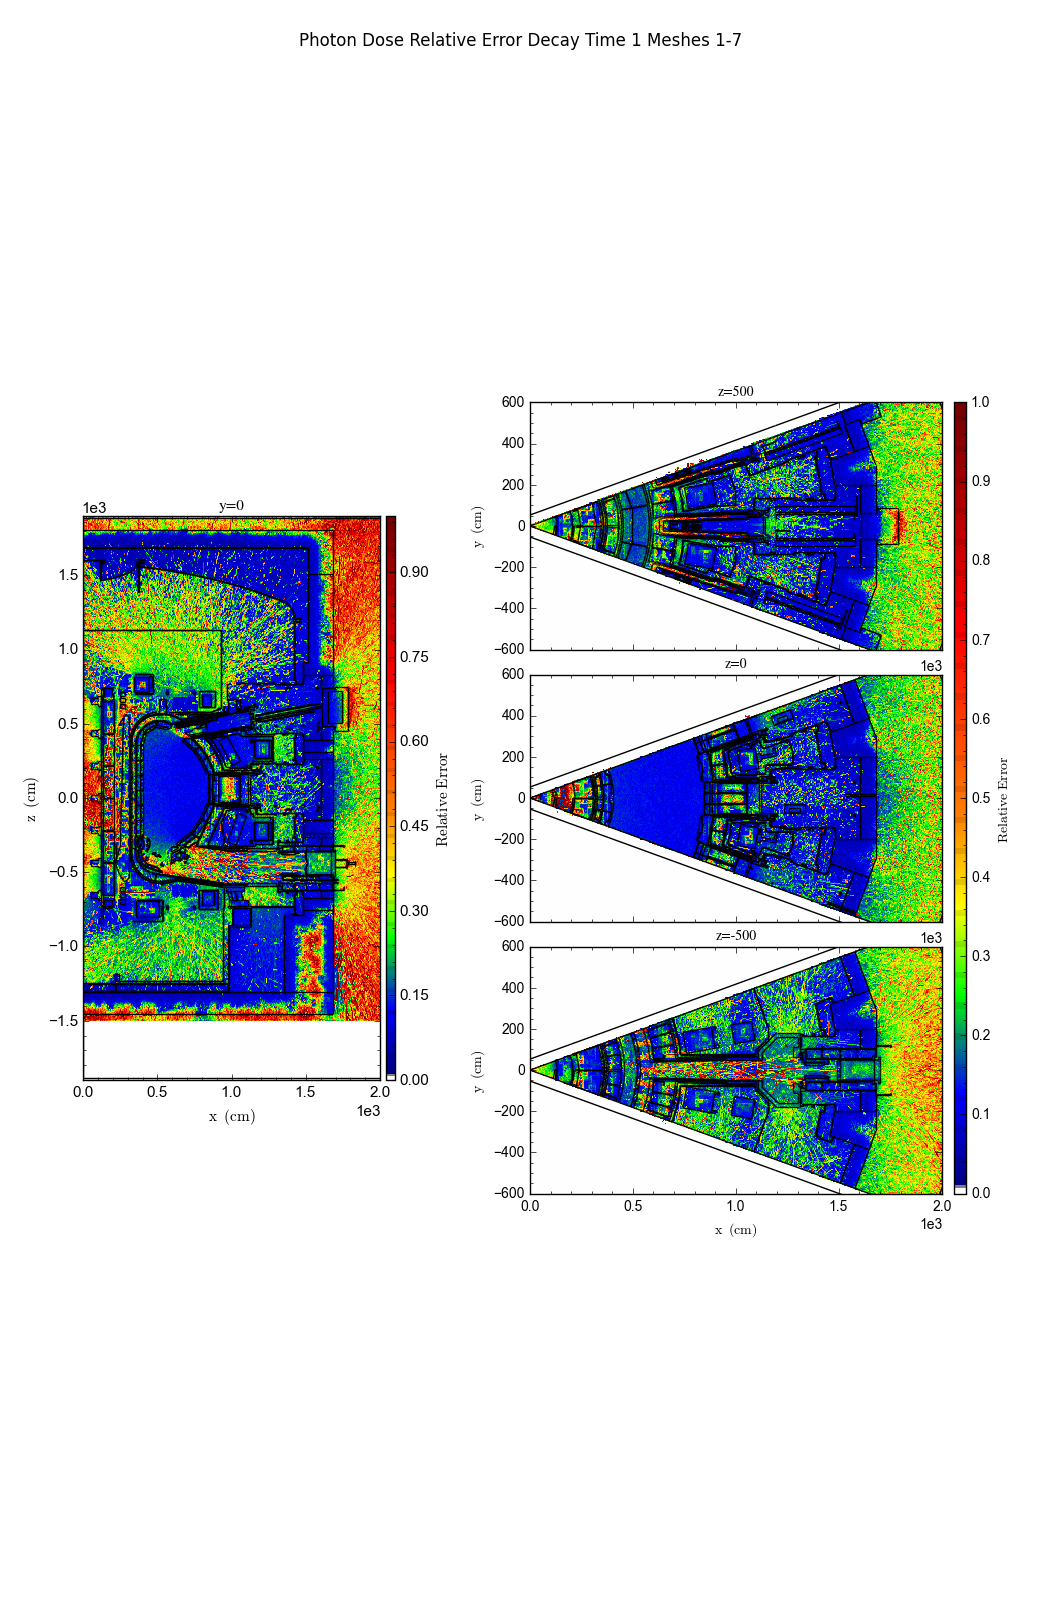
\includegraphics[trim={0cm 8cm, 0cm 8cm},clip,scale=0.75]{../plots/final_model_with_b4c/5year/Photon_Dose_Relative_Error_Decay_Time_1_Meshes_1-7.png}
\caption{Total dose rate relative error for decay time 1 for the ``SA-2 - 10 Yr'' irradiation}
\label{fig:photons_5y_dc1_b4c_relerr}
\end{figure}
\clearpage
\begin{figure}[ht!]
\centering
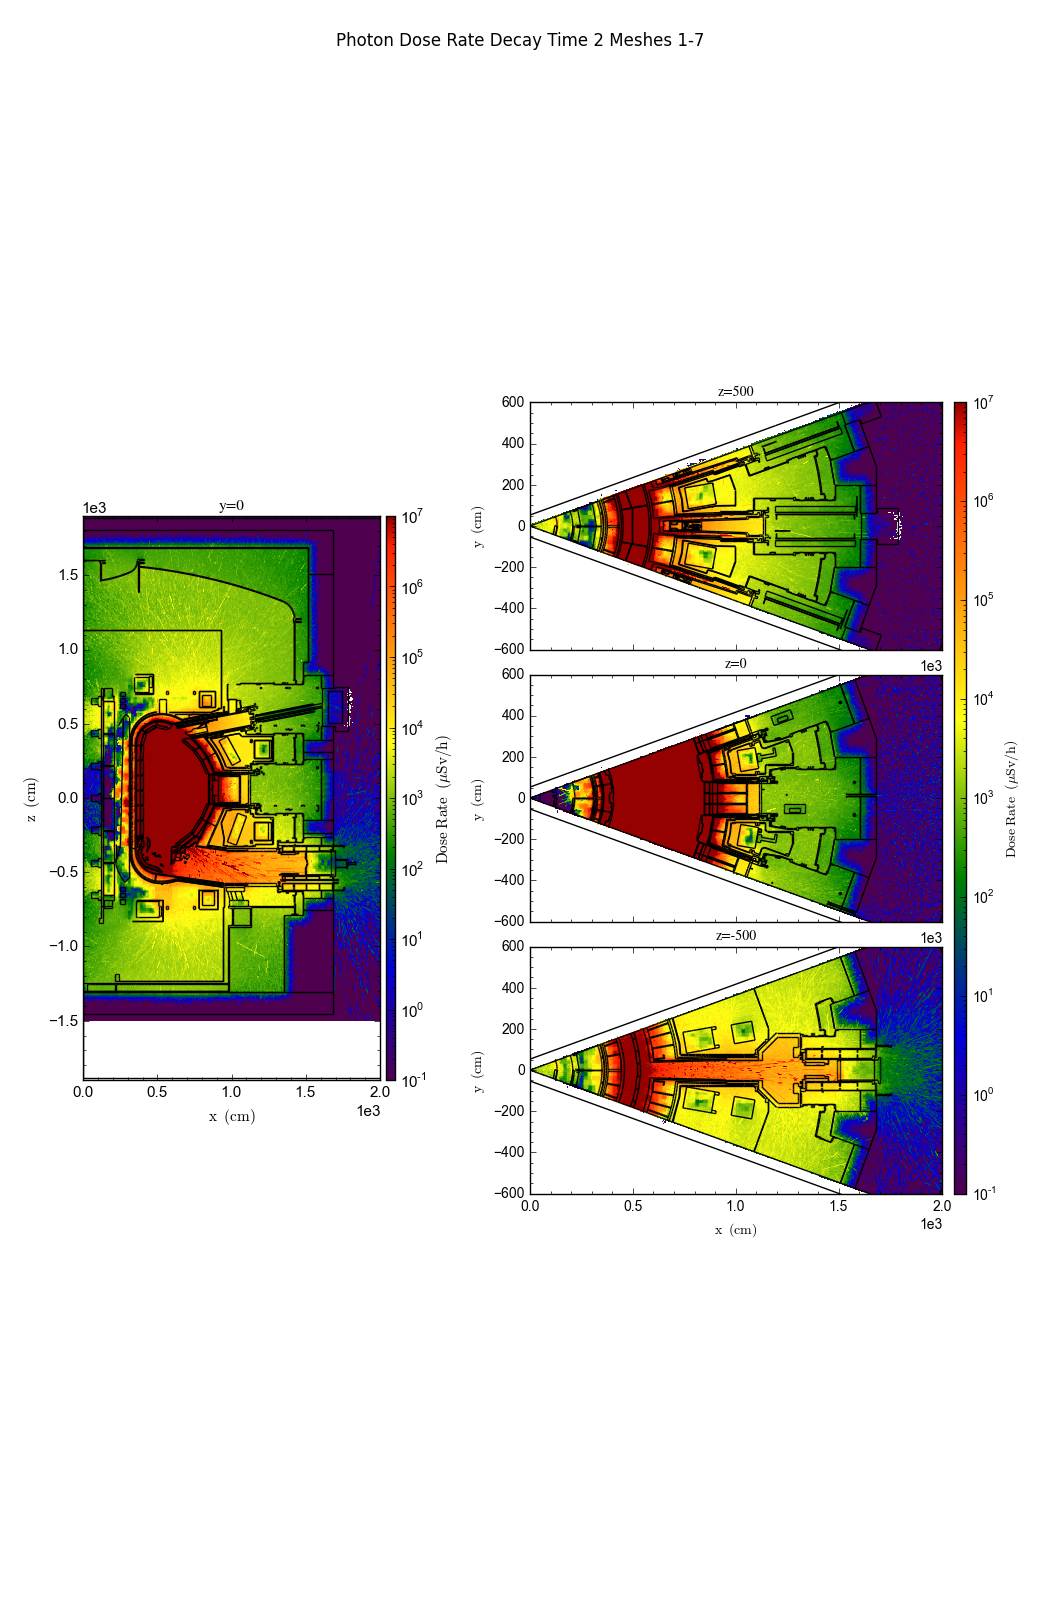
\includegraphics[trim={0cm 8cm, 0cm 8cm},clip,scale=0.75]{../plots/final_model_with_b4c/5year/Photon_Dose_Rate_Decay_Time_2_Meshes_1-7.png}
\caption{Total dose rate for decay time 2 for the ``SA-2 - 10 Yr'' irradiation}
\label{fig:photons_5y_dc2_b4c_dose}
\end{figure}
\begin{figure}[ht!]
\centering
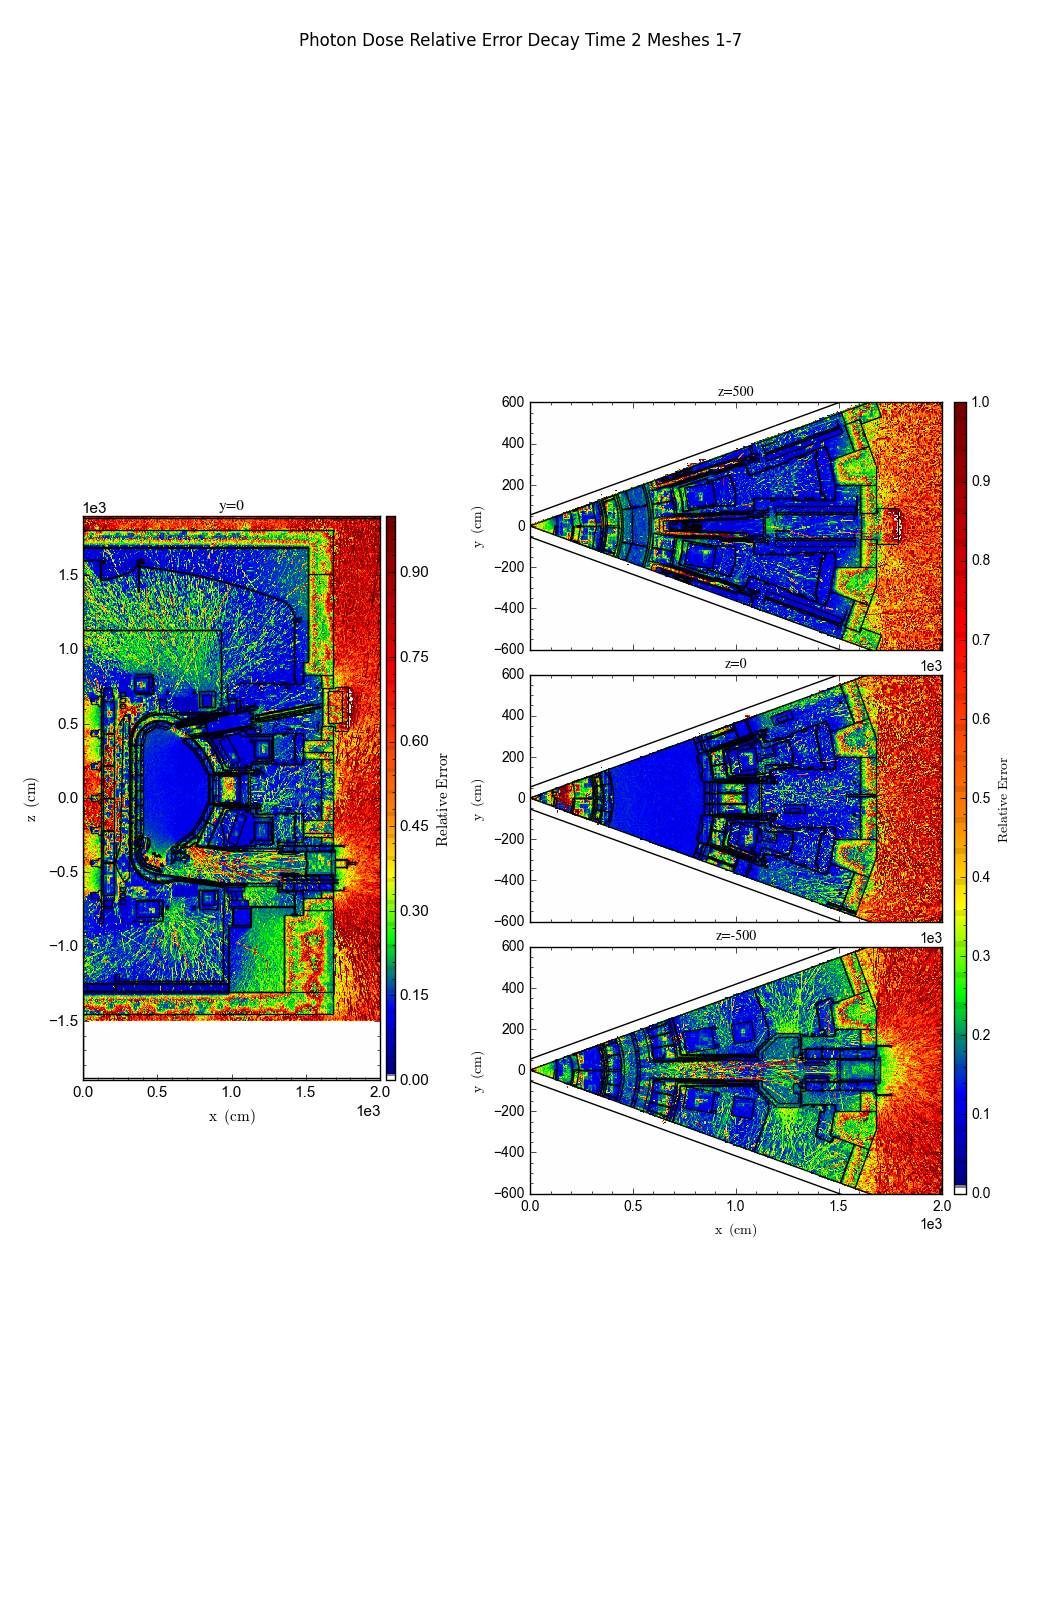
\includegraphics[trim={0cm 8cm, 0cm 8cm},clip,scale=0.75]{../plots/final_model_with_b4c/5year/Photon_Dose_Relative_Error_Decay_Time_2_Meshes_1-7.png}
\caption{Total dose rate relative error for decay time 2 for the ``SA-2 - 10 Yr'' irradiation}
\label{fig:photons_5y_dc2_b4c_relerr}
\end{figure}
\clearpage
\begin{figure}[ht!]
\centering
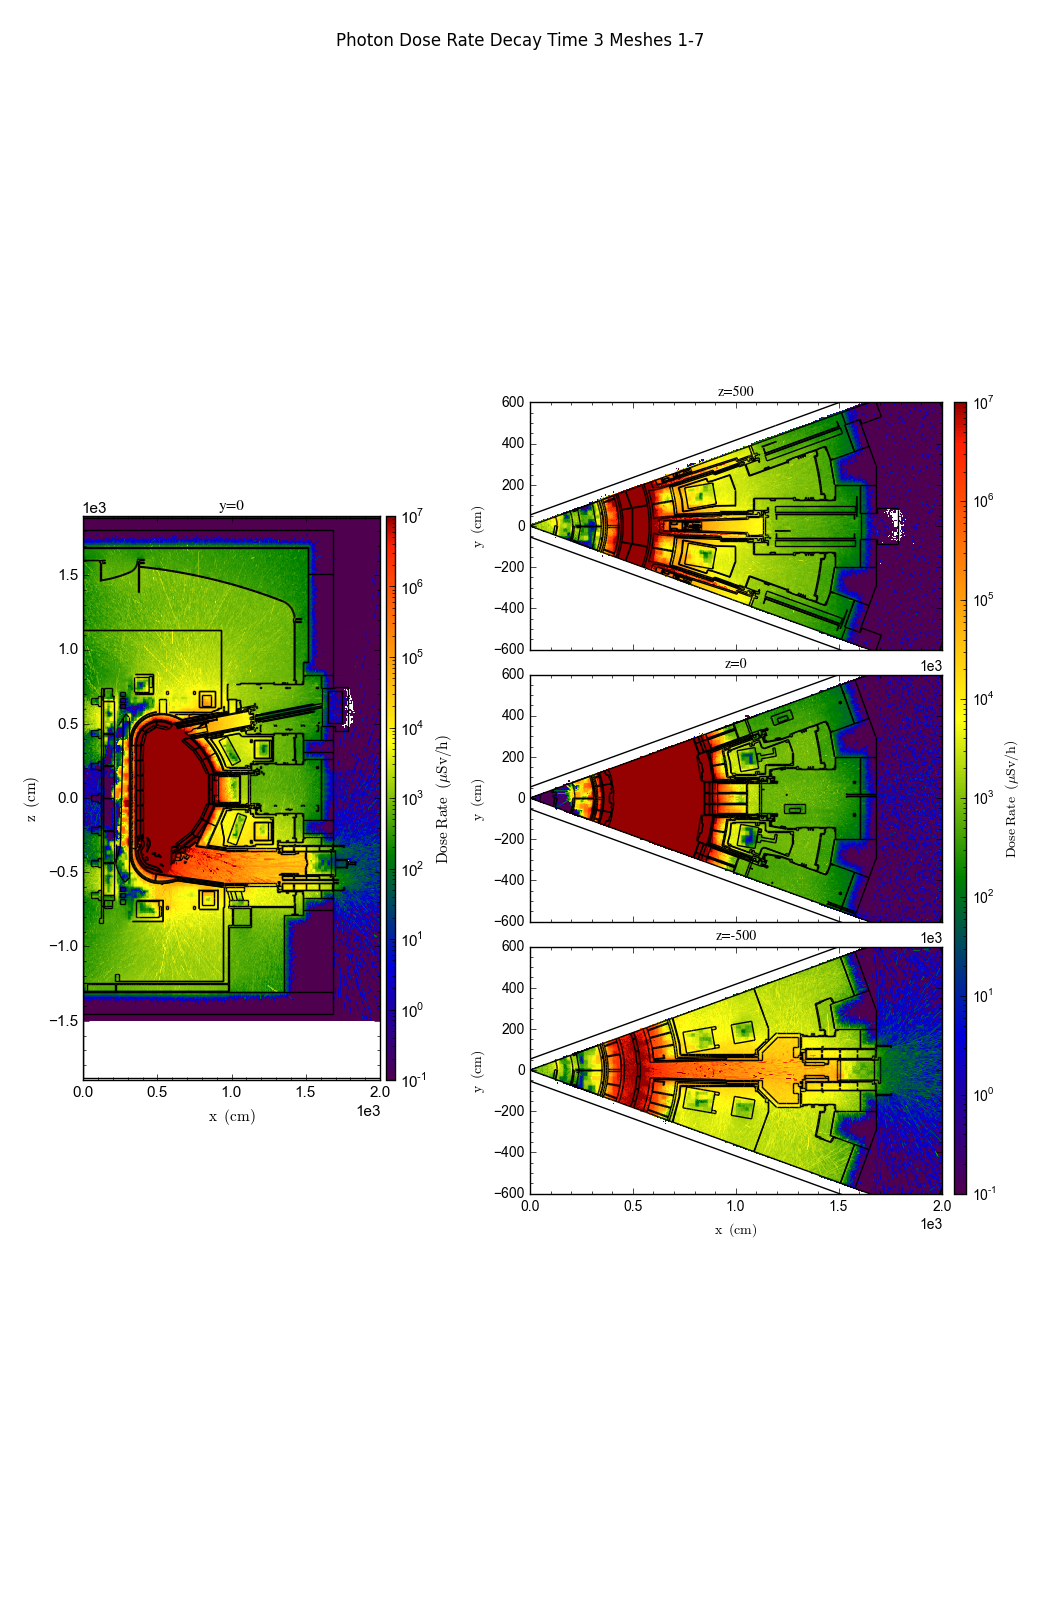
\includegraphics[trim={0cm 8cm, 0cm 8cm},clip,scale=0.75]{../plots/final_model_with_b4c/5year/Photon_Dose_Rate_Decay_Time_3_Meshes_1-7.png}
\caption{Total dose rate for decay time 3 for the ``SA-2 - 10 Yr'' irradiation}
\label{fig:photons_5y_dc3_b4c_dose}
\end{figure}
\begin{figure}[ht!]
\centering
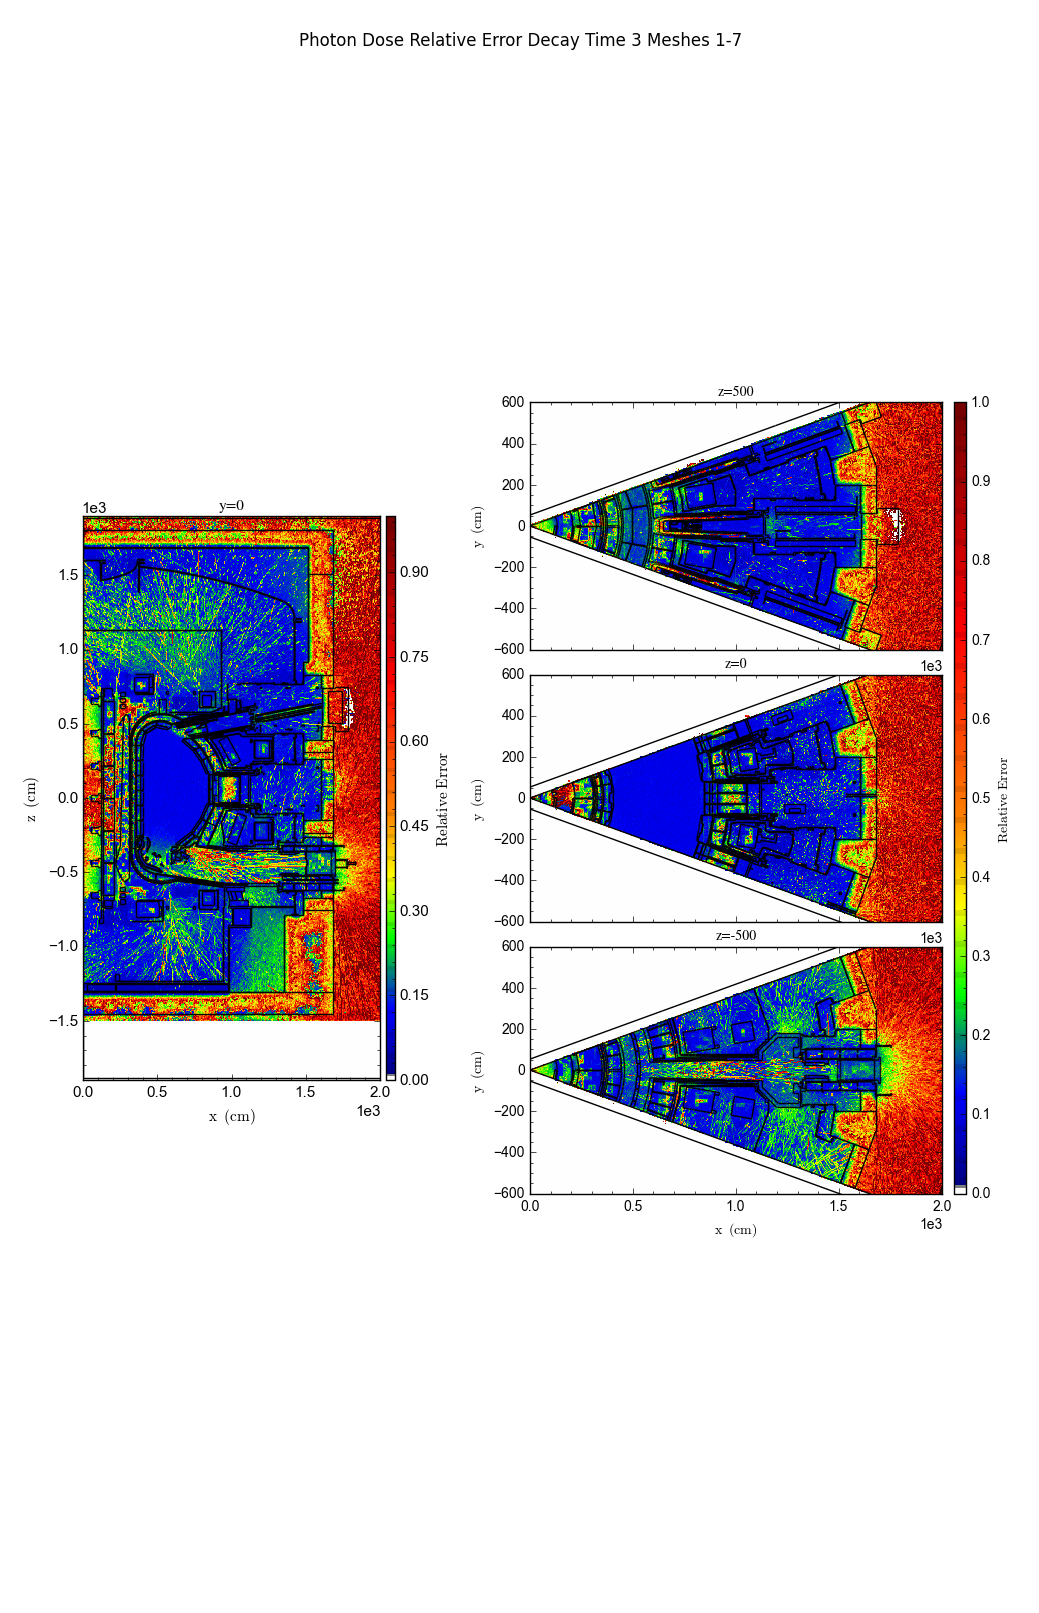
\includegraphics[trim={0cm 8cm, 0cm 8cm},clip,scale=0.75]{../plots/final_model_with_b4c/5year/Photon_Dose_Relative_Error_Decay_Time_3_Meshes_1-7.png}
\caption{Total dose rate relative error for decay time 3 for the ``SA-2 - 10 Yr'' irradiation}
\label{fig:photons_5y_dc3_b4c_relerr}
\end{figure}
\clearpage
\newpage
\section{Appendix B - B4C ``SA-2 - 5 Yr'' Irradiation}
\begin{figure}[ht!]
\centering
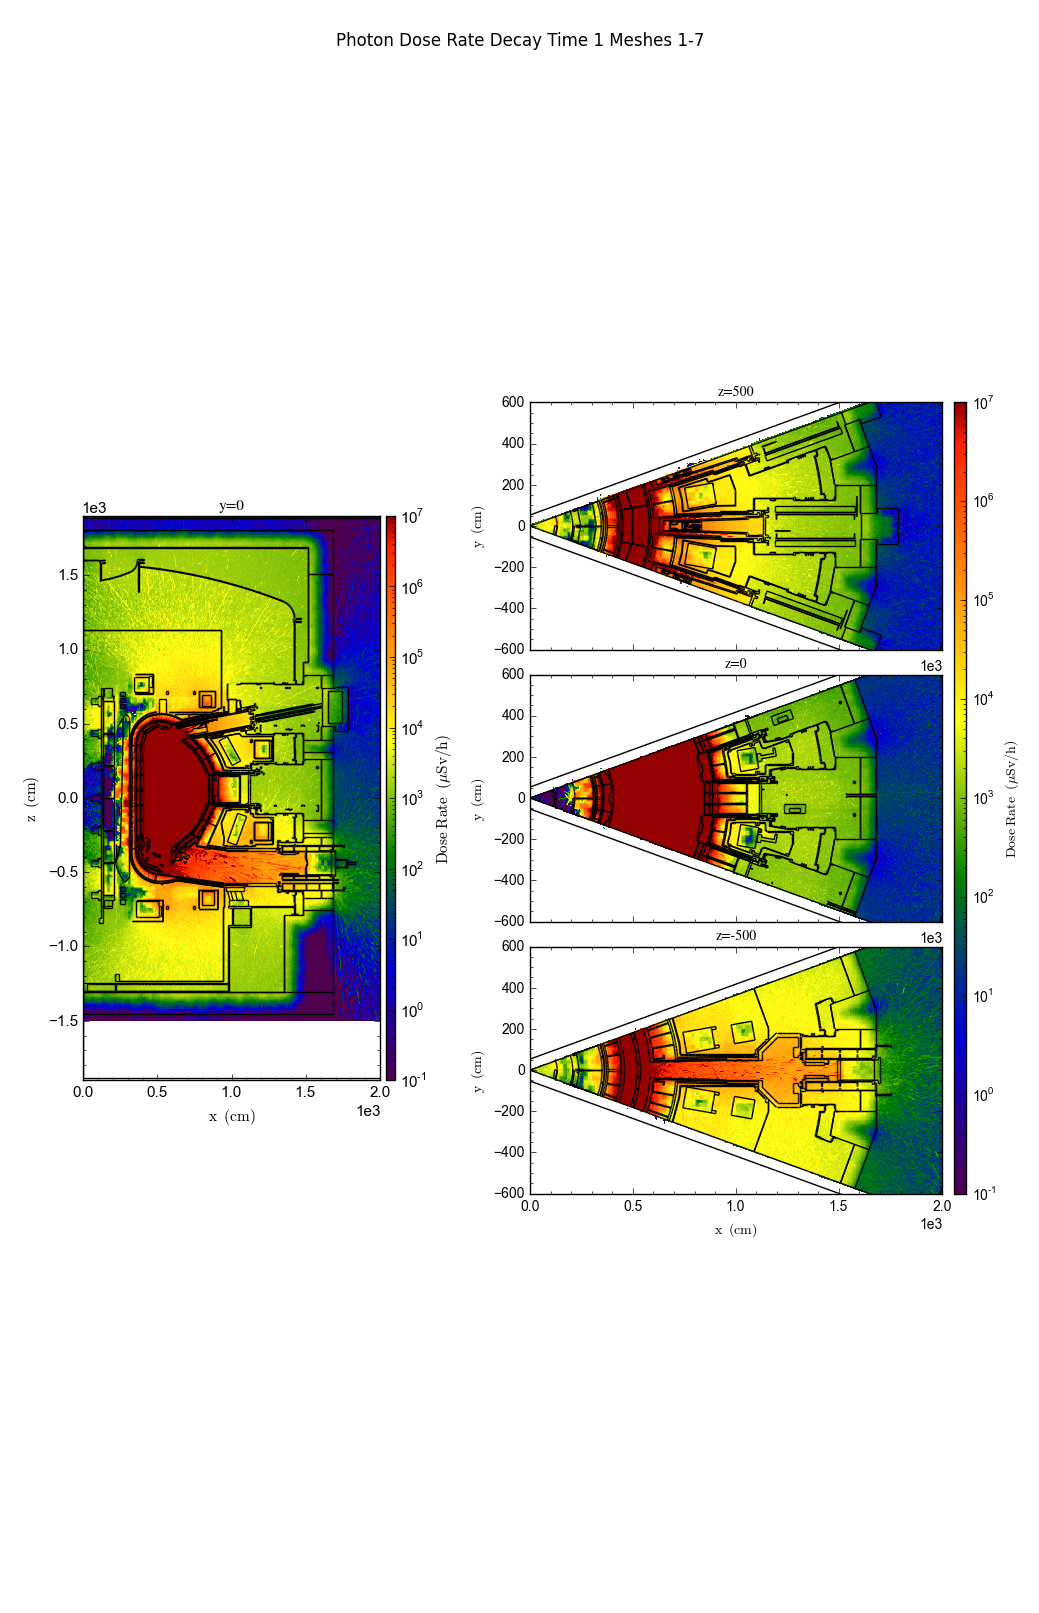
\includegraphics[trim={0cm 8cm, 0cm 8cm},clip,scale=0.75]{../plots/final_model_with_b4c/10year/Photon_Dose_Rate_Decay_Time_1_Meshes_1-7.png}
\caption{Total dose rate for decay time 1 for the ``SA-2 - 5 Yr'' irradiation}
\label{fig:photons_10y_dc1_b4c_dose}
\end{figure}
\begin{figure}[ht!]
\centering
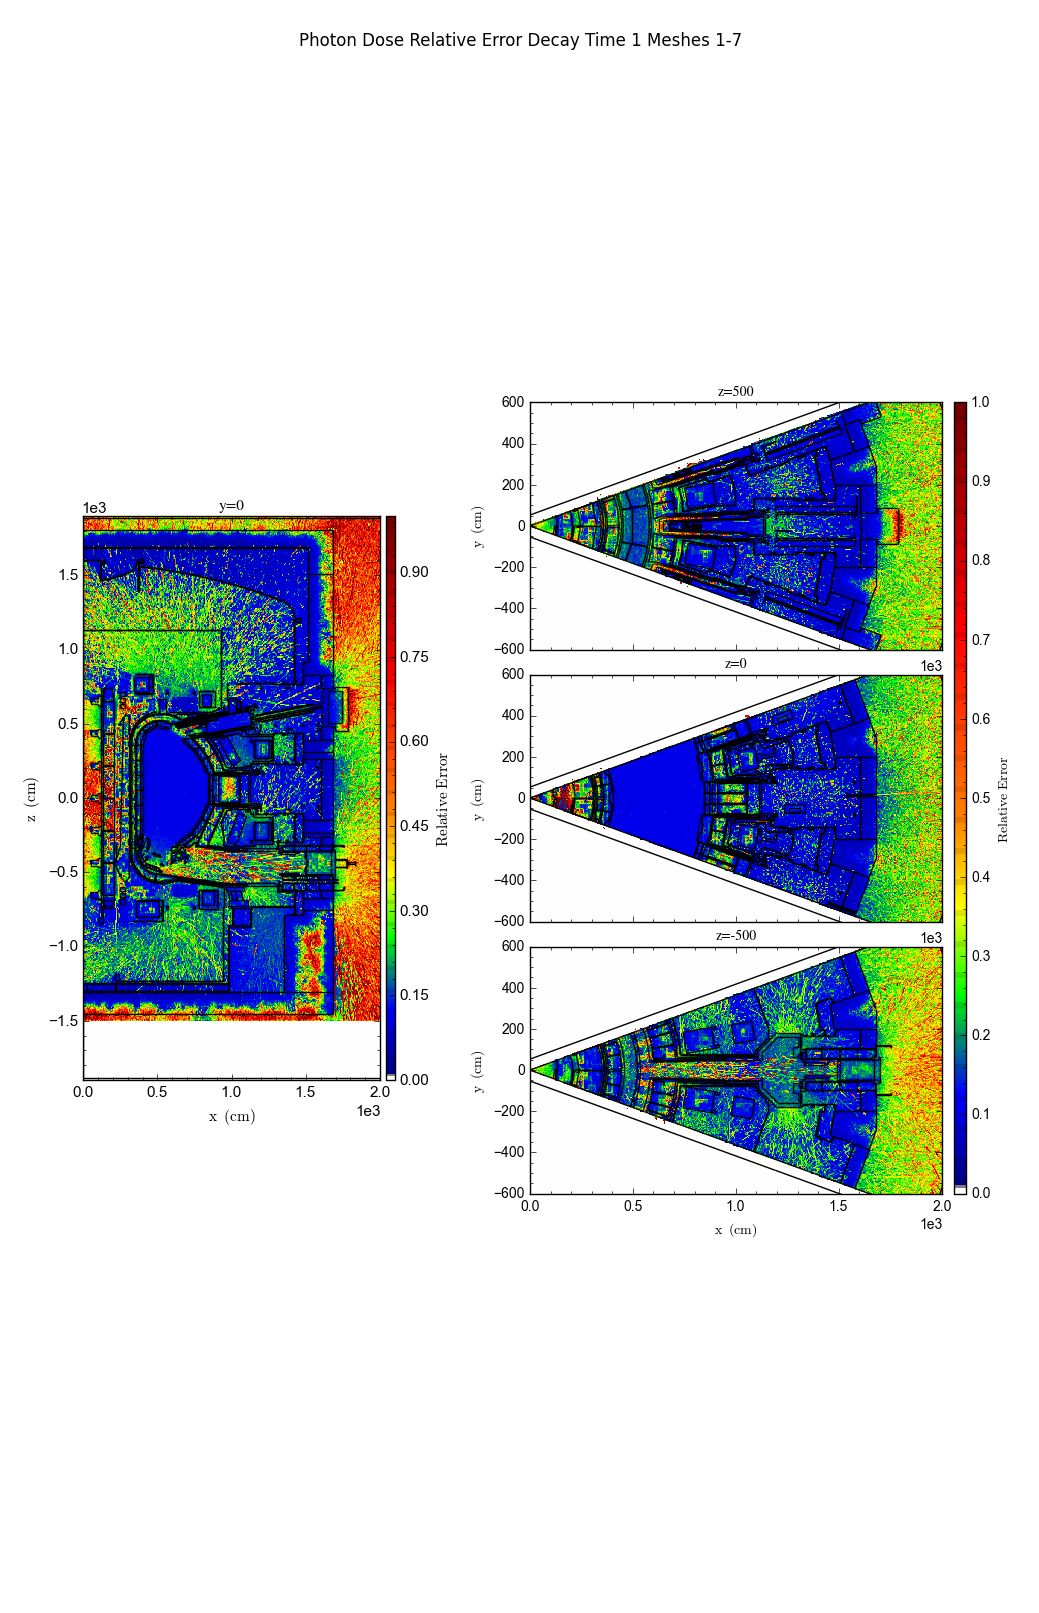
\includegraphics[trim={0cm 8cm, 0cm 8cm},clip,scale=0.75]{../plots/final_model_with_b4c/10year/Photon_Dose_Relative_Error_Decay_Time_1_Meshes_1-7.png}
\caption{Total dose rate relative error for decay time 1 for the ``SA-2 - 5 Yr'' irradiation}
\label{fig:photons_10y_dc1_b4c_relerr}
\end{figure}
\clearpage
\begin{figure}[ht!]
\centering
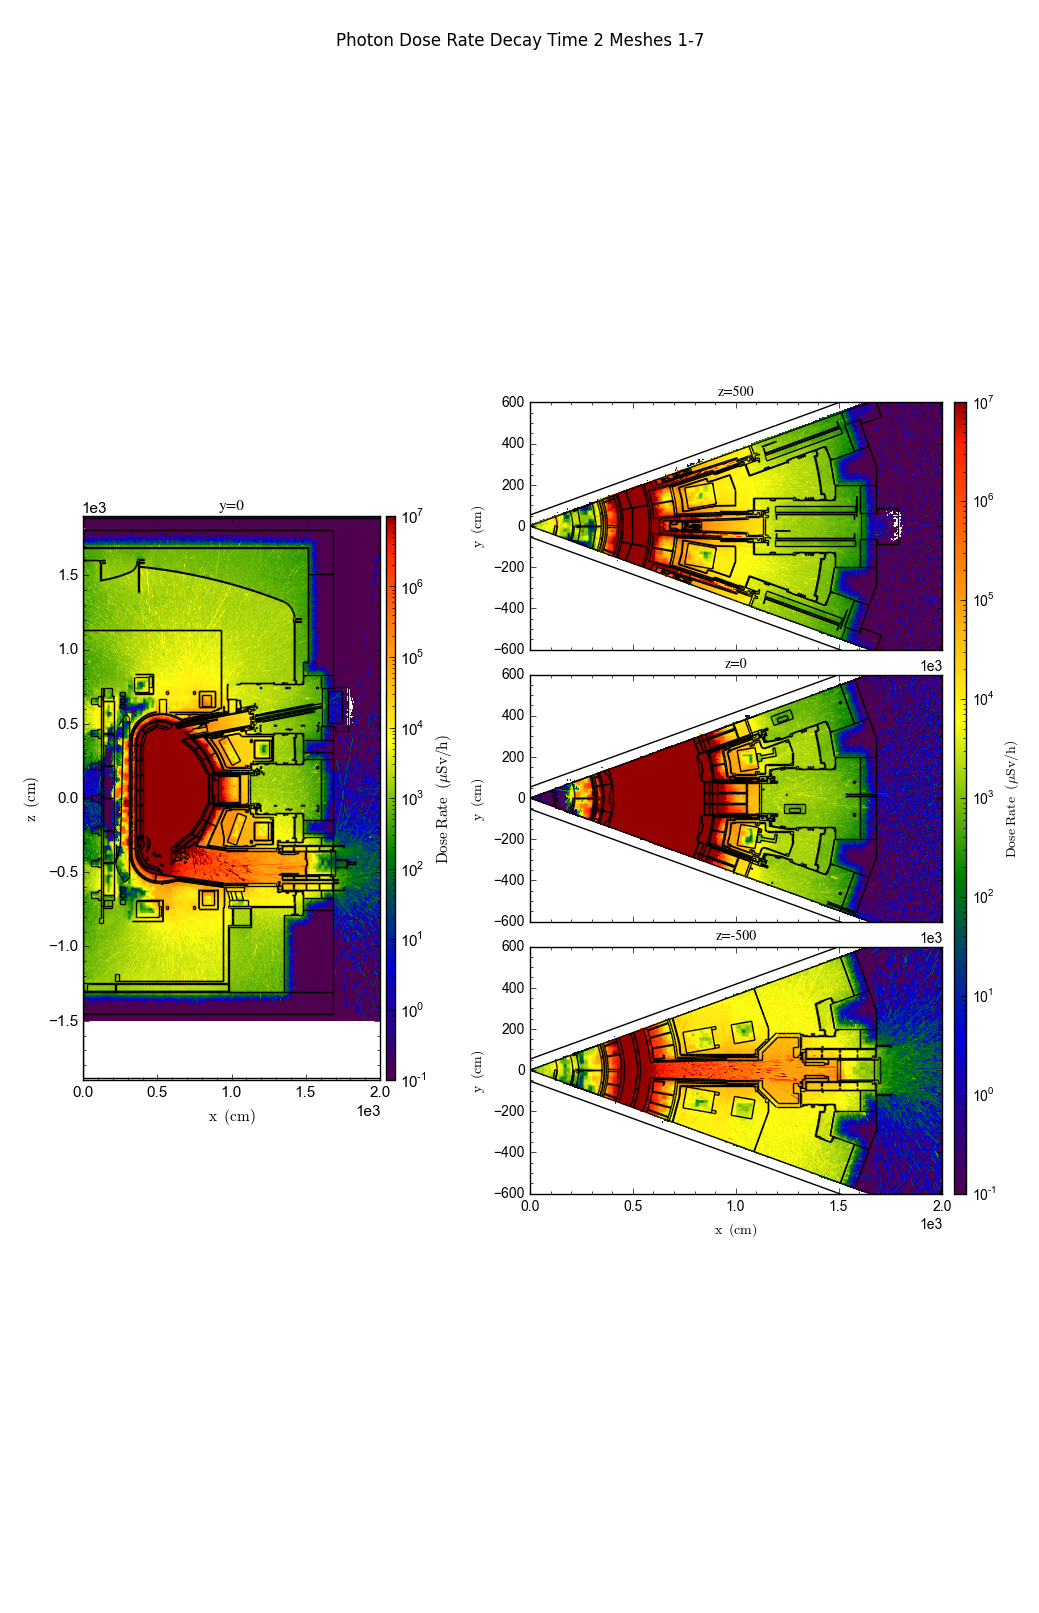
\includegraphics[trim={0cm 8cm, 0cm 8cm},clip,scale=0.75]{../plots/final_model_with_b4c/10year/Photon_Dose_Rate_Decay_Time_2_Meshes_1-7.png}
\caption{Total dose rate for decay time 2 for the ``SA-2 - 5 Yr'' irradiation}
\label{fig:photons_10y_dc2_b4c_dose}
\end{figure}
\begin{figure}[ht!]
\centering
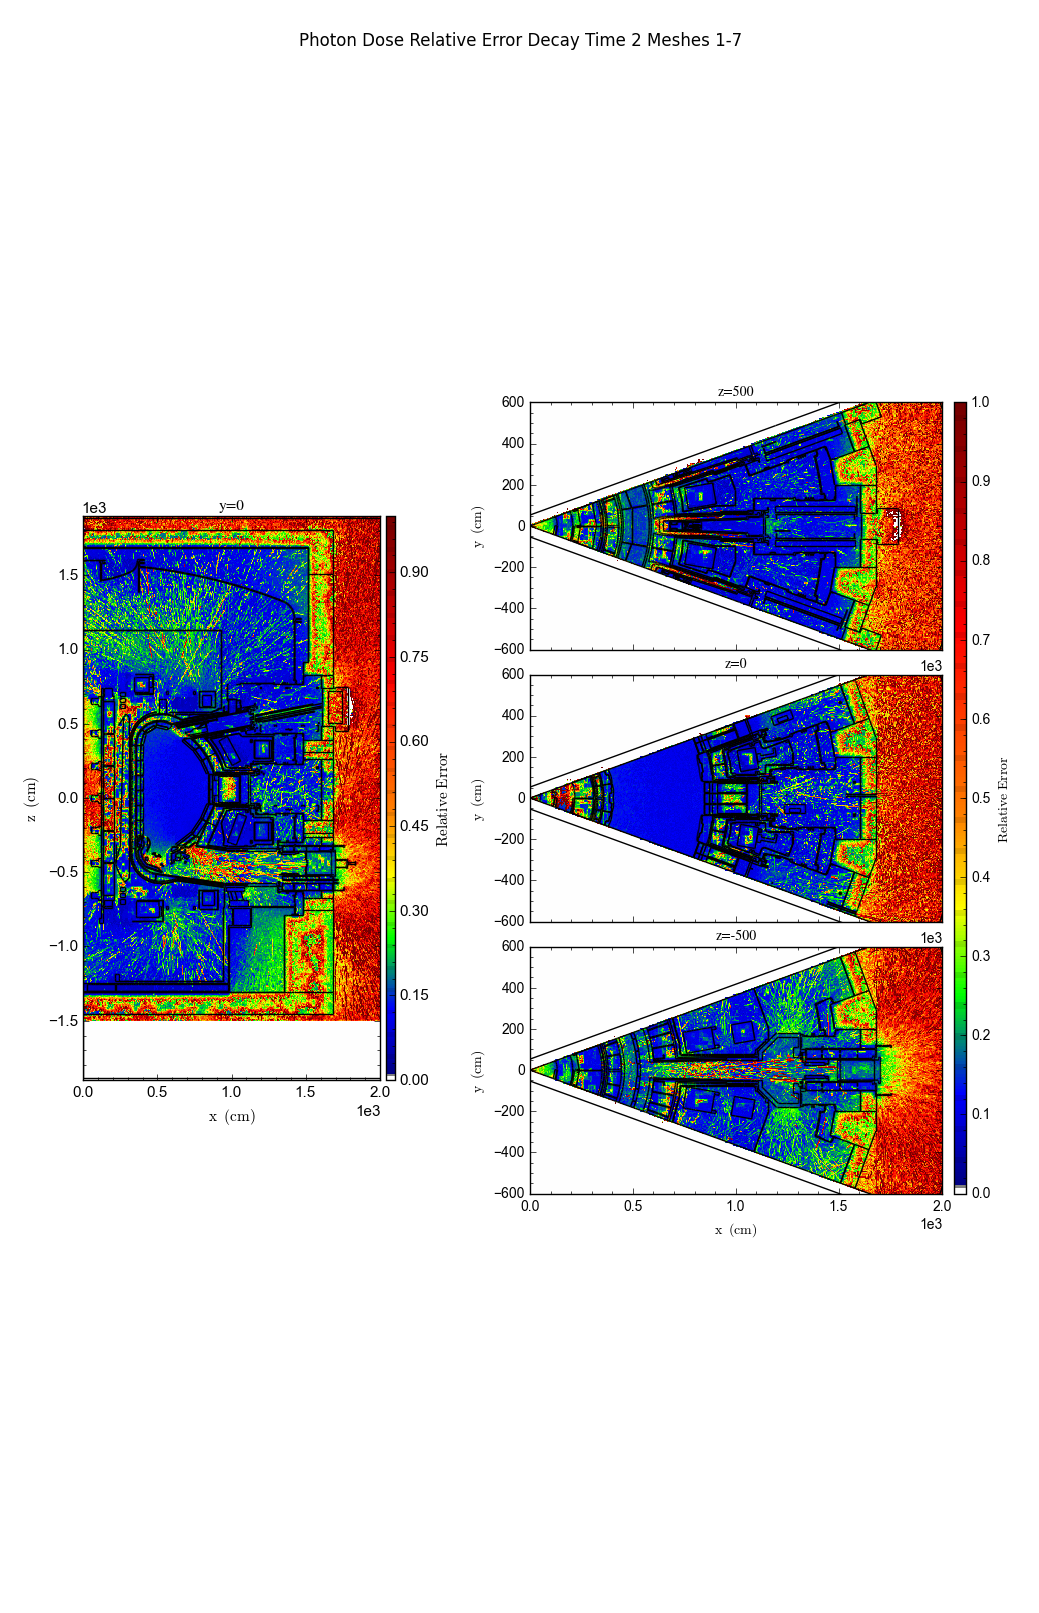
\includegraphics[trim={0cm 8cm, 0cm 8cm},clip,scale=0.75]{../plots/final_model_with_b4c/10year/Photon_Dose_Relative_Error_Decay_Time_2_Meshes_1-7.png}
\caption{Total dose rate relative error for decay time 2 for the ``SA-2 - 5 Yr'' irradiation}
\label{fig:photons_10y_dc2_b4c_relerr}
\end{figure}

\clearpage
\begin{figure}[ht!]
\centering
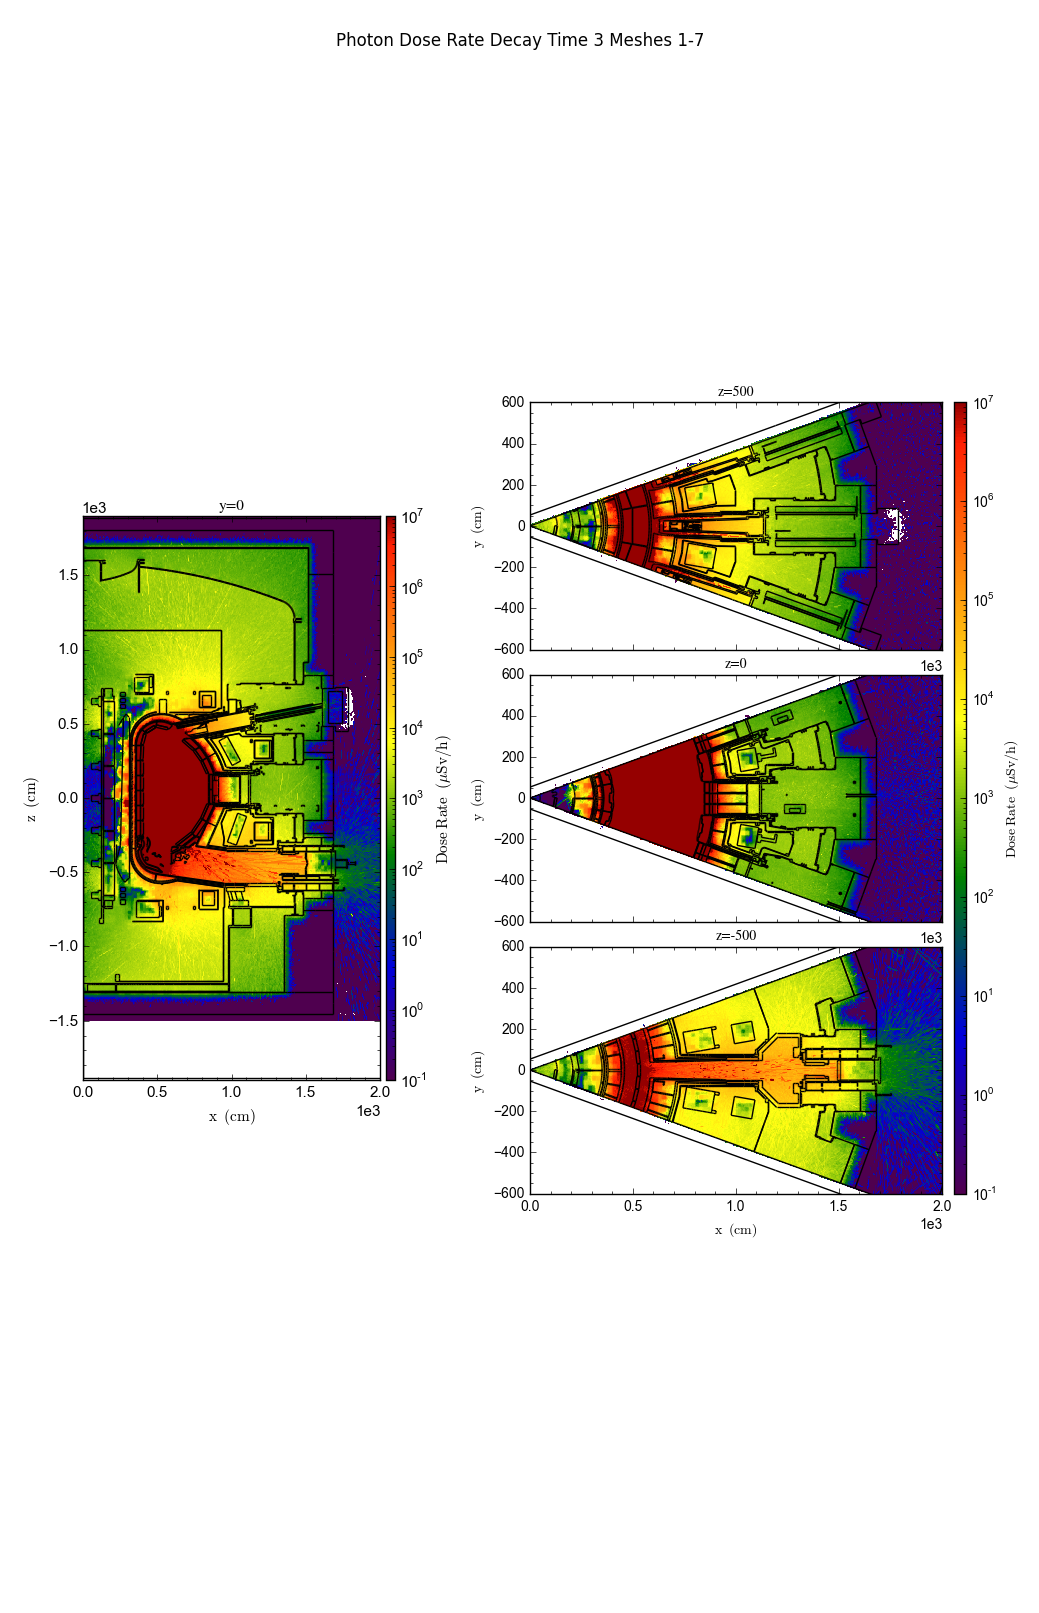
\includegraphics[trim={0cm 8cm, 0cm 8cm},clip,scale=0.75]{../plots/final_model_with_b4c/10year/Photon_Dose_Rate_Decay_Time_3_Meshes_1-7.png}
\caption{Total dose rate for decay time 3 for the ``SA-2 - 5 Yr'' irradiation}
\label{fig:photons_10y_dc3_b4c_dose}
\end{figure}
\begin{figure}[ht!]
\centering
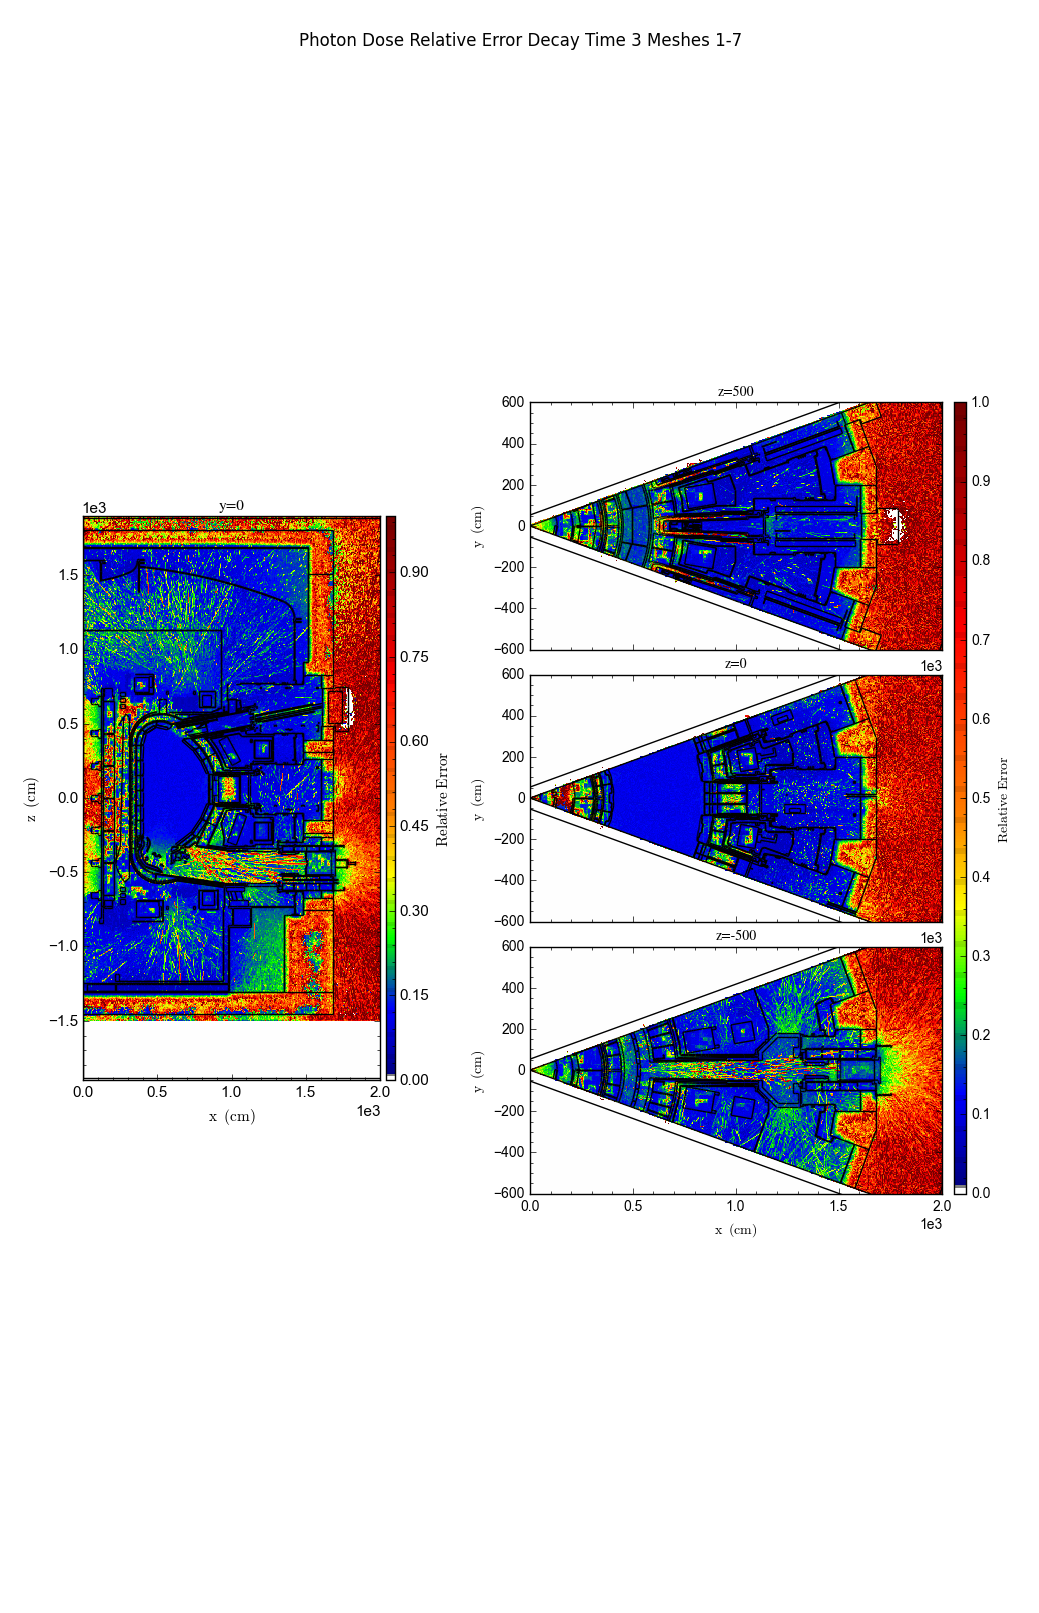
\includegraphics[trim={0cm 8cm, 0cm 8cm},clip,scale=0.75]{../plots/final_model_with_b4c/10year/Photon_Dose_Relative_Error_Decay_Time_3_Meshes_1-7.png}
\caption{Total dose rate relative error for decay time 3 for the ``SA-2 - 5 Yr'' irradiation}
\label{fig:photons_10y_dc3_b4c_relerr}
\end{figure}
\newpage
\section{Appendix C - No B4C ``SA-2 - 10 Yr'' Irradiation}
\begin{figure}[ht!]
\centering
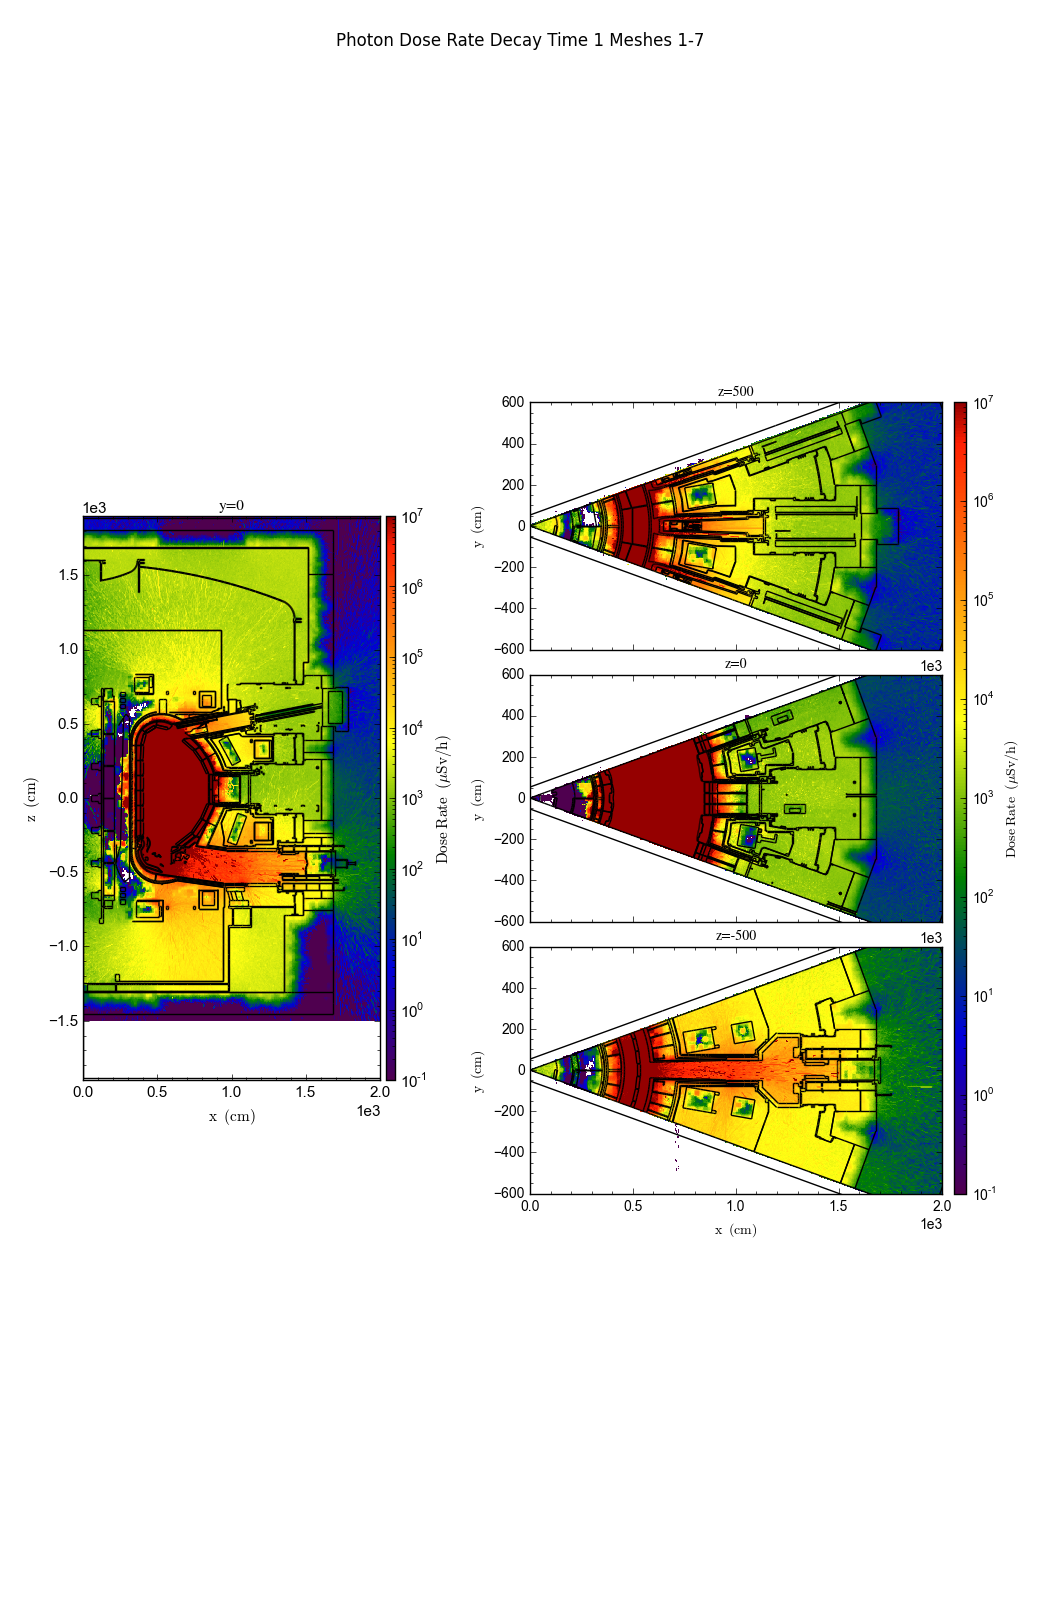
\includegraphics[trim={0cm 8cm, 0cm 8cm},clip,scale=0.75]{../plots/final_model/5year/Photon_Dose_Rate_Decay_Time_1_Meshes_1-7.png}
\caption{Total dose rate for decay time 1 for the ``SA-2 - 10 Yr'' irradiation}
\label{fig:photons_5y_dc1_nob4c_dose}
\end{figure}
\begin{figure}[ht!]
\centering
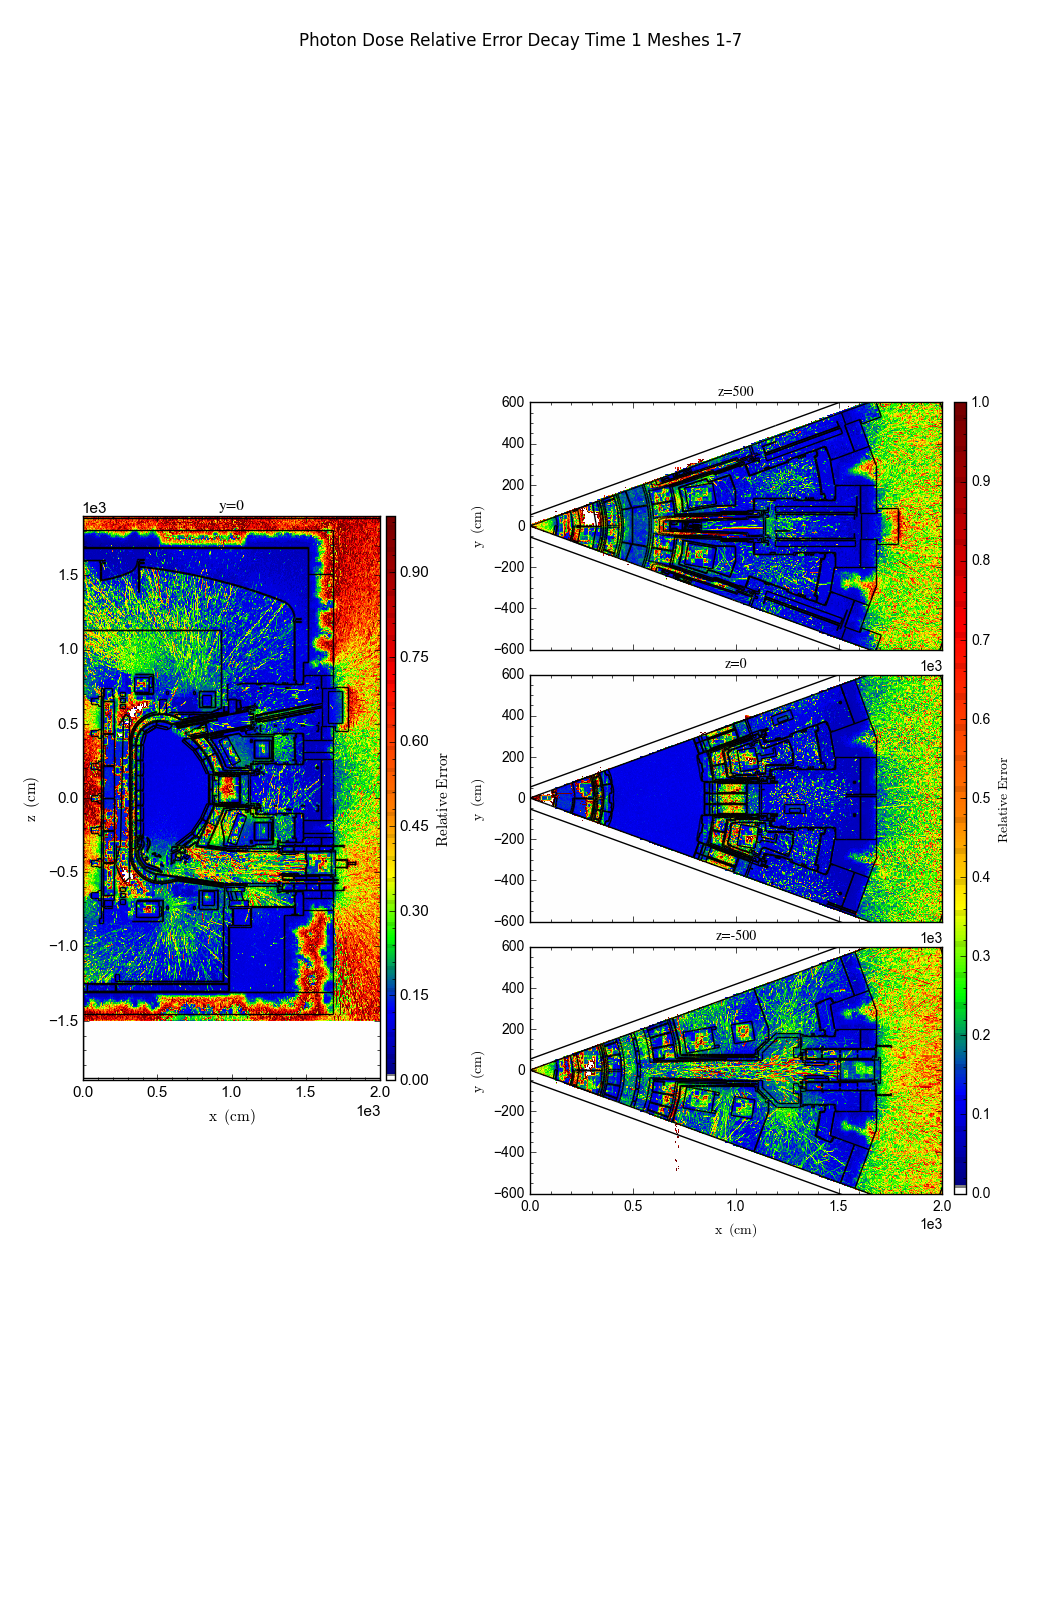
\includegraphics[trim={0cm 8cm, 0cm 8cm},clip,scale=0.75]{../plots/final_model/5year/Photon_Dose_Relative_Error_Decay_Time_1_Meshes_1-7.png}
\caption{Total dose rate relative error for decay time 1 for the ``SA-2 - 10 Yr'' irradiation}
\label{fig:photons_5y_dc1_nob4c_relerr}
\end{figure}
\clearpage
\begin{figure}[ht!]
\centering
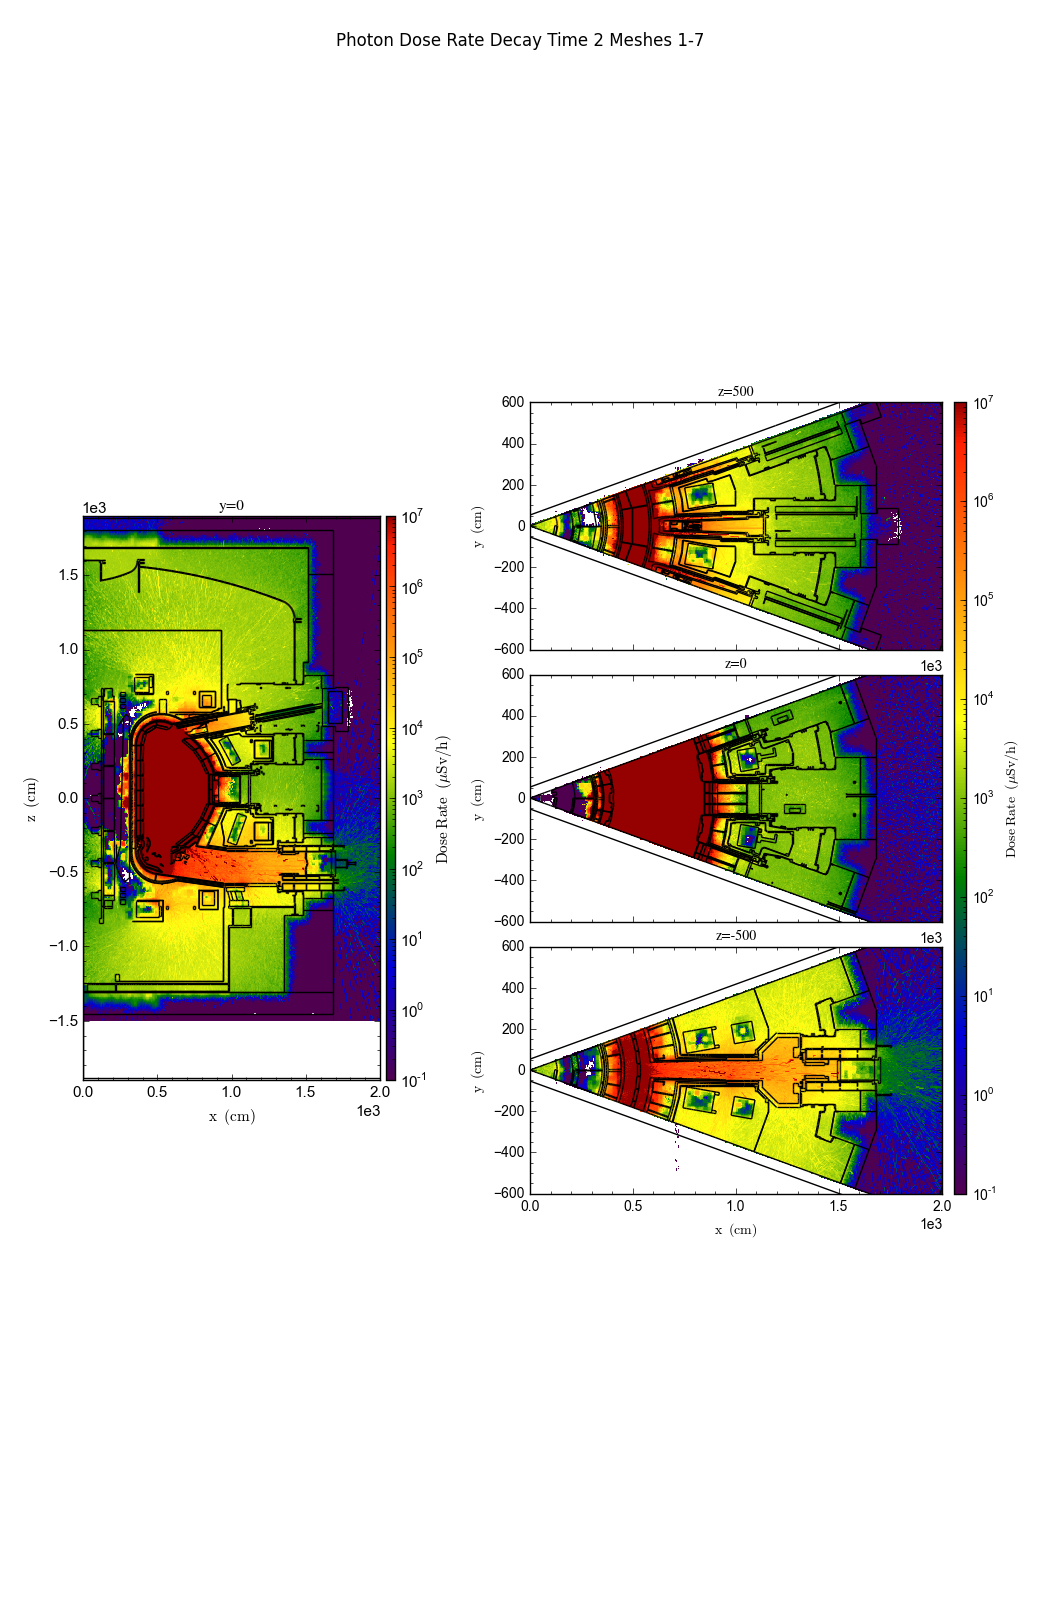
\includegraphics[trim={0cm 8cm, 0cm 8cm},clip,scale=0.75]{../plots/final_model/5year/Photon_Dose_Rate_Decay_Time_2_Meshes_1-7.png}
\caption{Total dose rate for decay time 2 for the ``SA-2 - 10 Yr'' irradiation}
\label{fig:photons_5y_dc2_nob4c_dose}
\end{figure}
\begin{figure}[ht!]
\centering
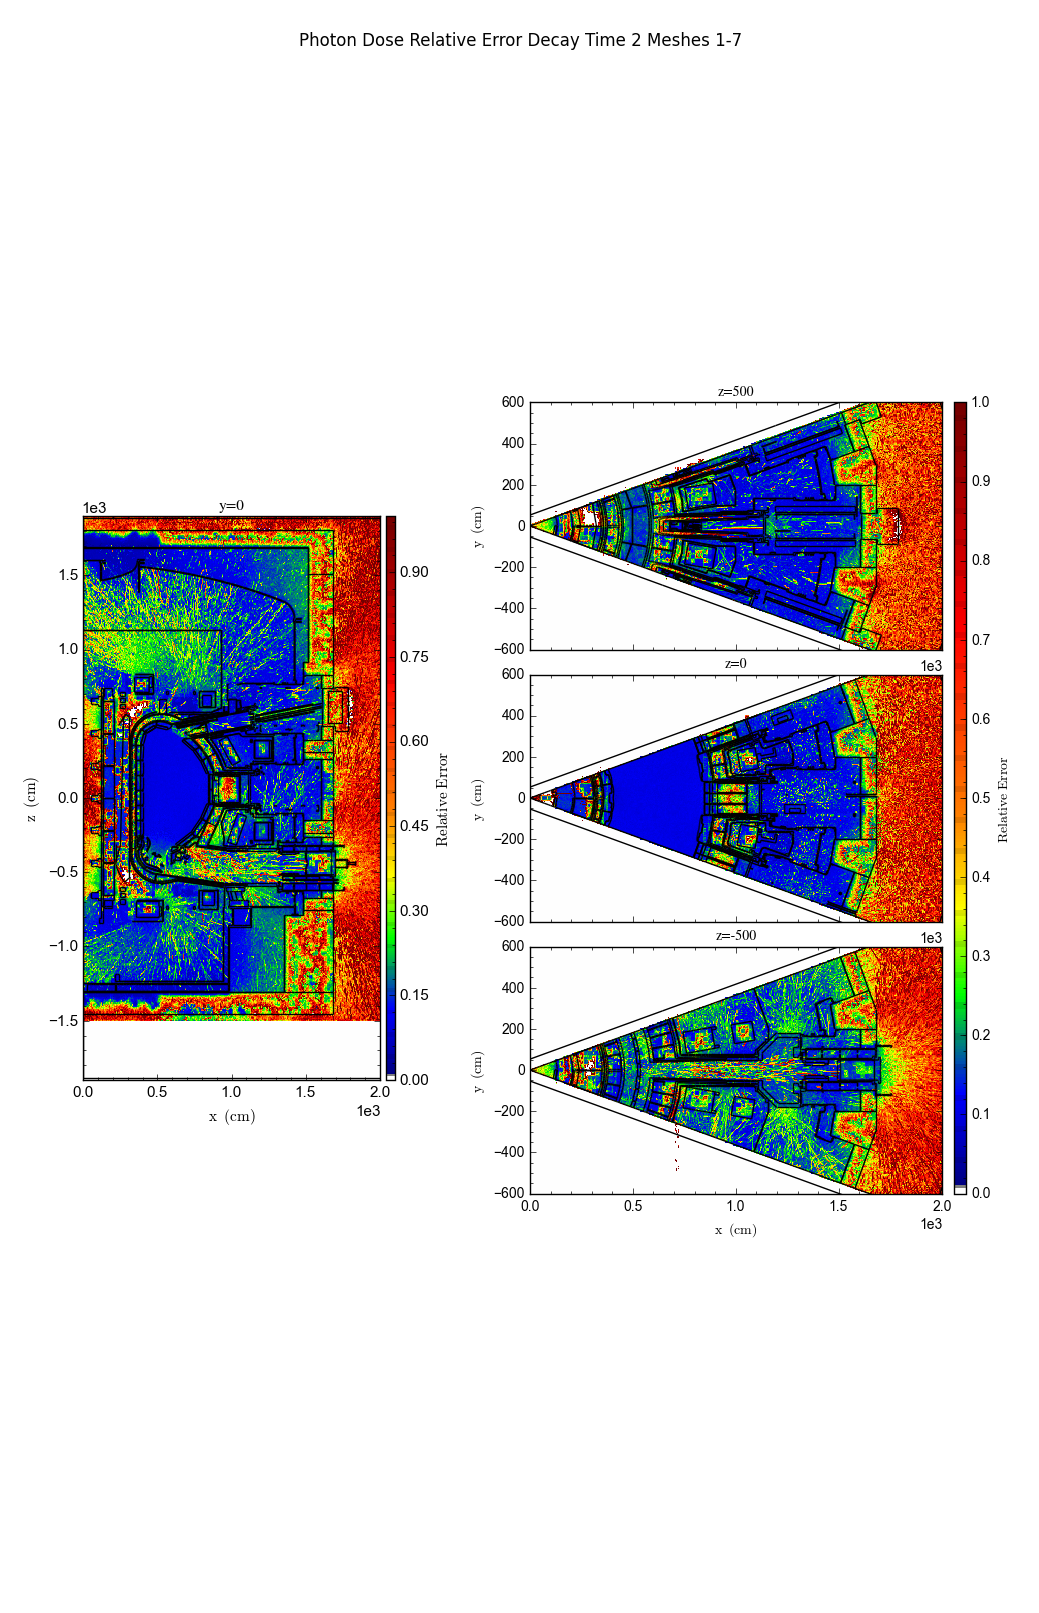
\includegraphics[trim={0cm 8cm, 0cm 8cm},clip,scale=0.75]{../plots/final_model/5year/Photon_Dose_Relative_Error_Decay_Time_2_Meshes_1-7.png}
\caption{Total dose rate relative error for decay time 2 for the ``SA-2 - 10 Yr'' irradiation}
\label{fig:photons_5y_dc2_nob4c_relerr}
\end{figure}
\clearpage
\begin{figure}[ht!]
\centering
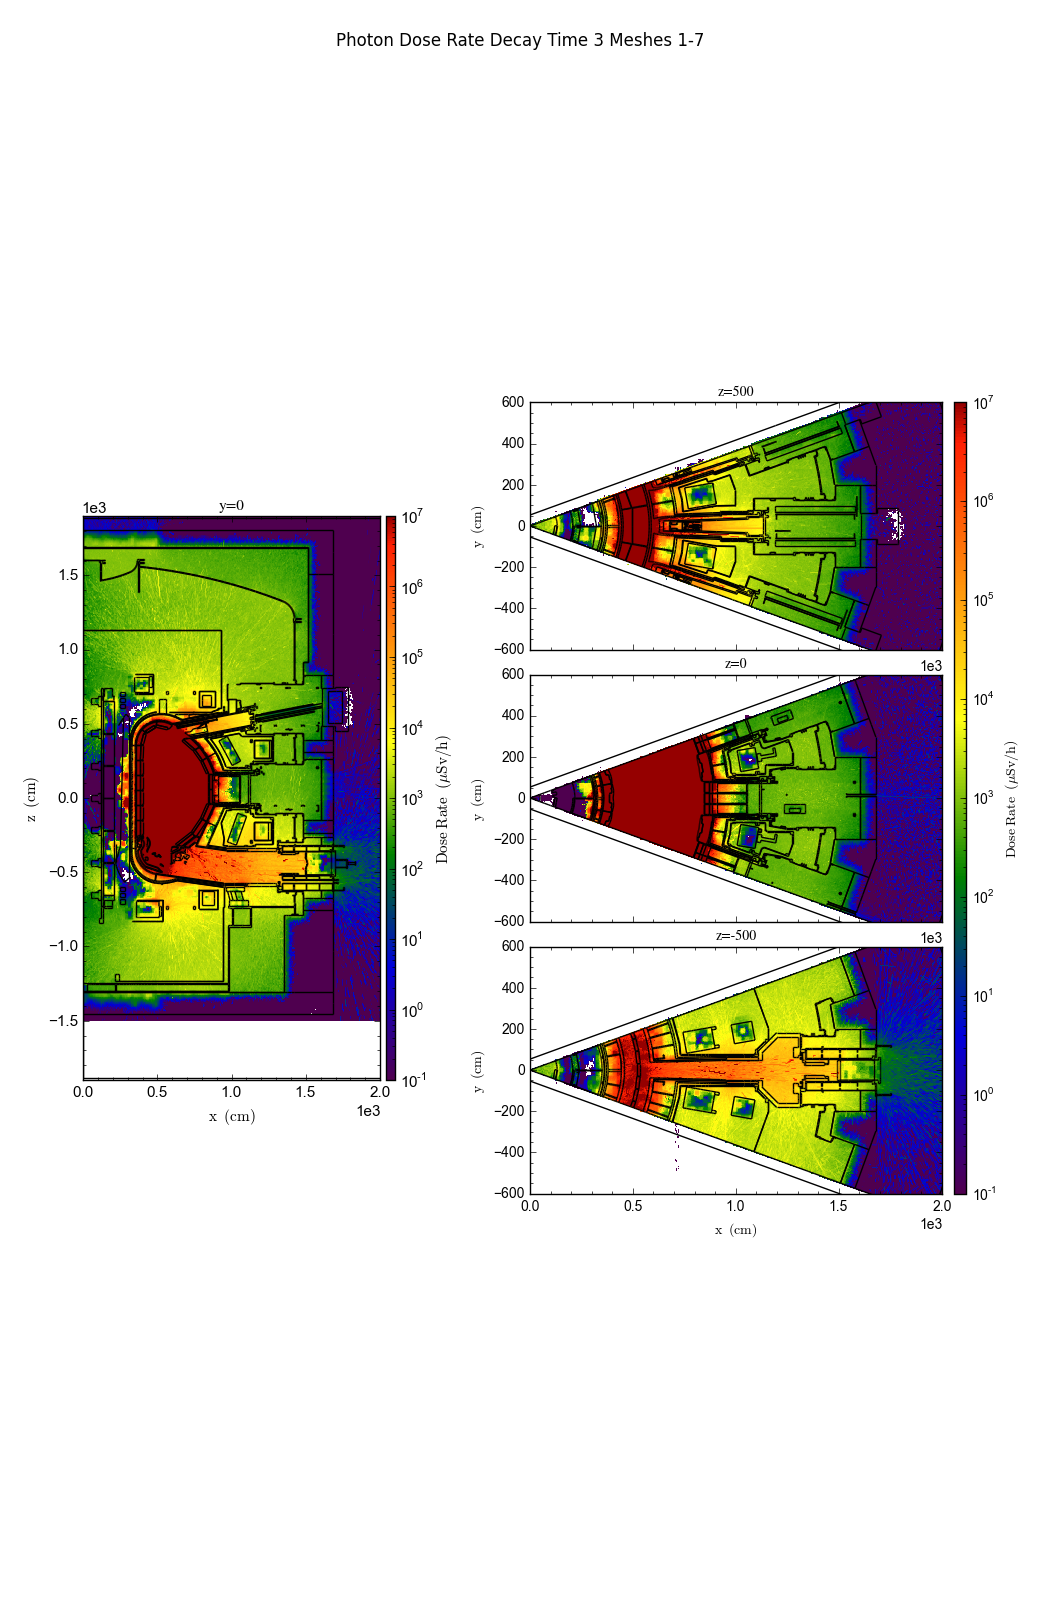
\includegraphics[trim={0cm 8cm, 0cm 8cm},clip,scale=0.75]{../plots/final_model/5year/Photon_Dose_Rate_Decay_Time_3_Meshes_1-7.png}
\caption{Total dose rate for decay time 3 for the ``SA-2 - 10 Yr'' irradiation}
\label{fig:photons_5y_dc3_nob4c_dose}
\end{figure}
\begin{figure}[ht!]
\centering
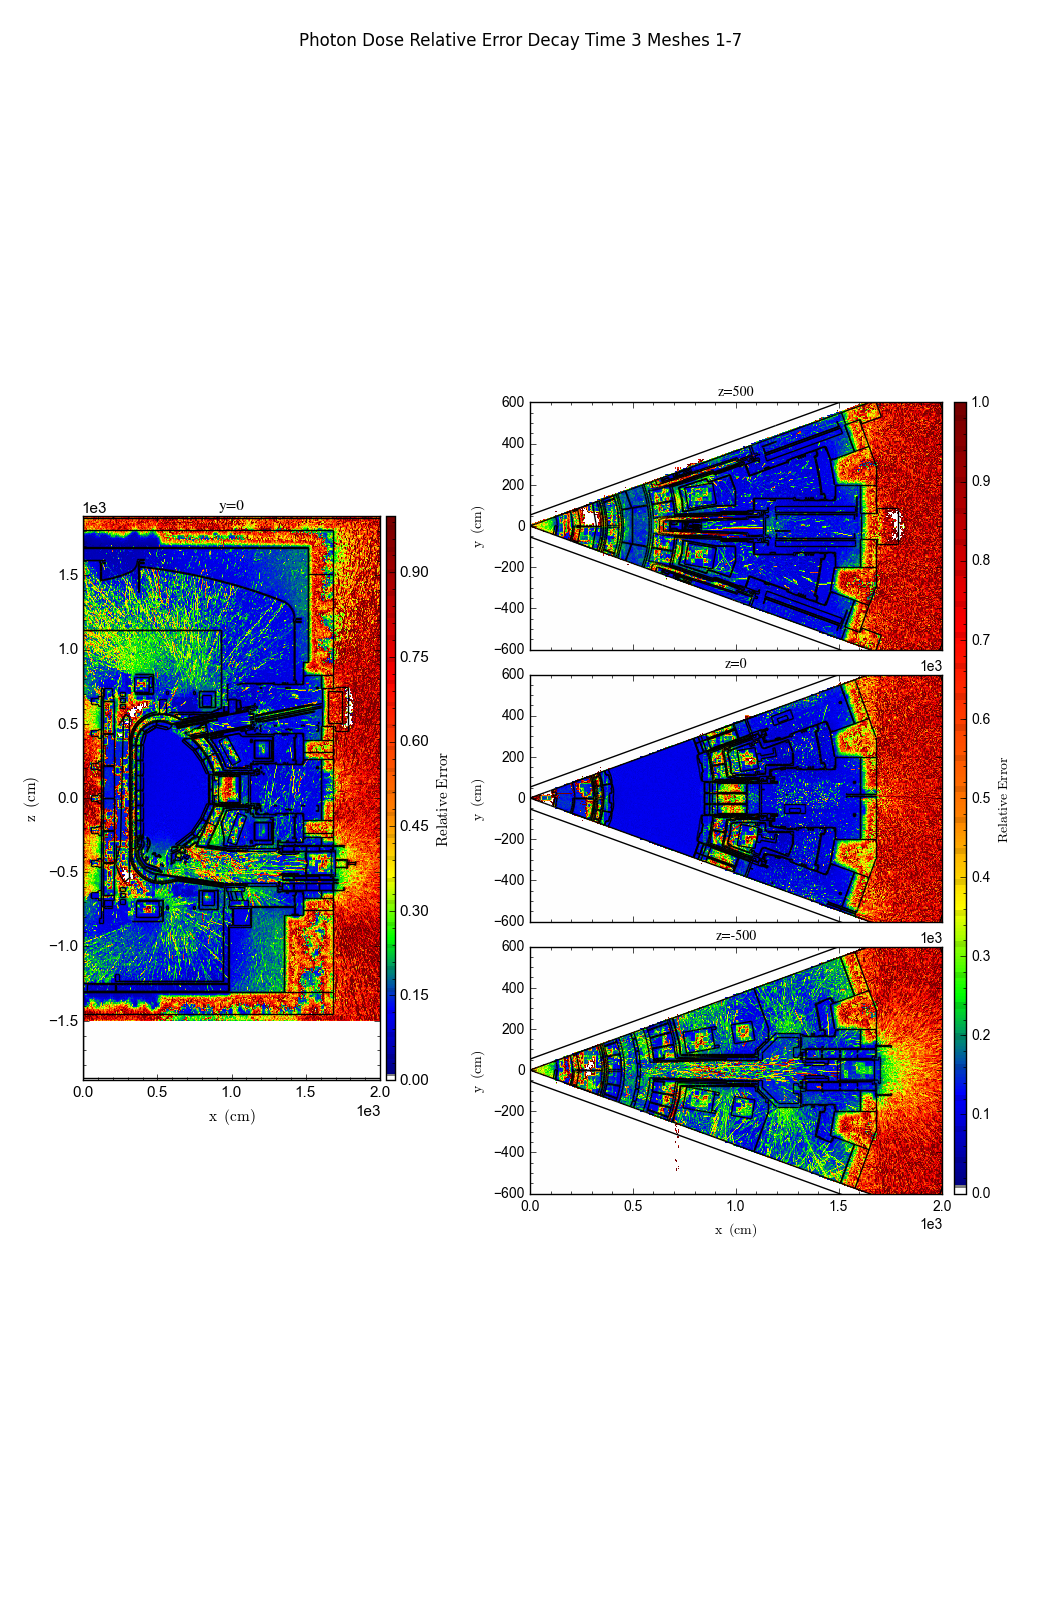
\includegraphics[trim={0cm 8cm, 0cm 8cm},clip,scale=0.75]{../plots/final_model/5year/Photon_Dose_Relative_Error_Decay_Time_3_Meshes_1-7.png}
\caption{Total dose rate relative error for decay time 3 for the ``SA-2 - 10 Yr'' irradiation}
\label{fig:photons_5y_dc3_nob4c_relerr}
\end{figure}
\clearpage
\newpage
\section{Appendix D - No B4C ``SA-2 - 5 Yr'' Irradiation}
\begin{figure}[ht!]
\centering
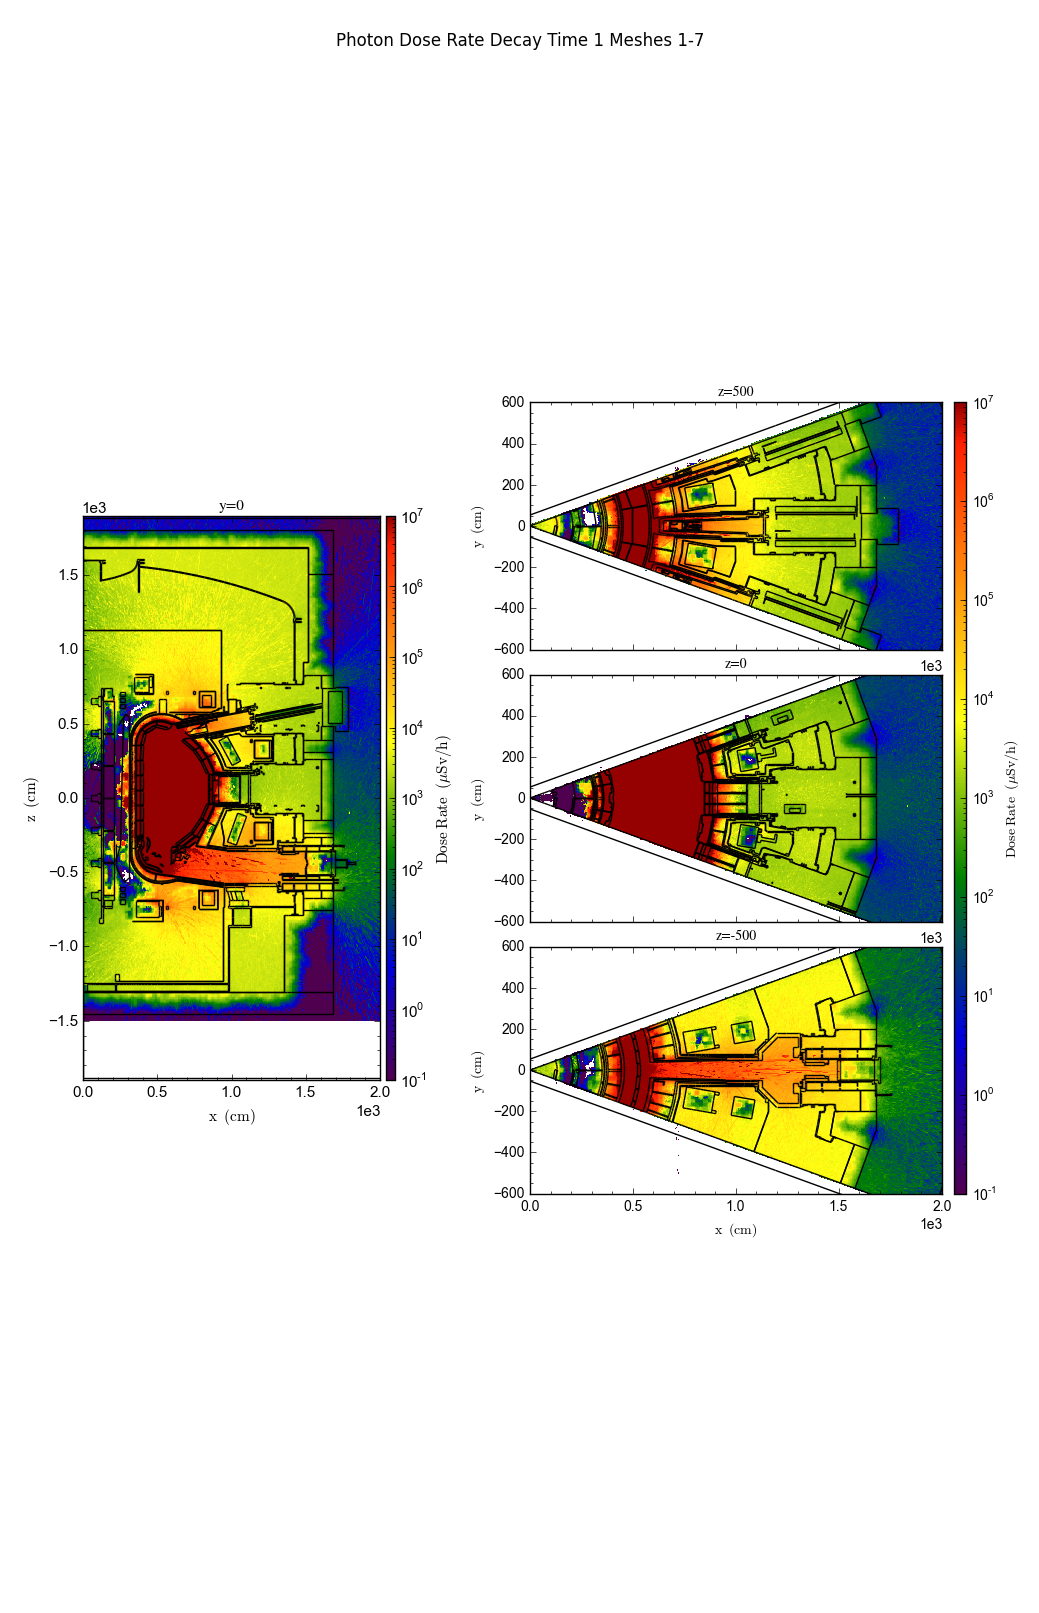
\includegraphics[trim={0cm 8cm, 0cm 8cm},clip,scale=0.75]{../plots/final_model/10year/Photon_Dose_Rate_Decay_Time_1_Meshes_1-7.png}
\caption{Total dose rate for decay time 1 for the ``SA-2 - 5 Yr'' irradiation}
\label{fig:photons_10y_dc1_nob4c_dose}
\end{figure}
\begin{figure}[ht!]
\centering
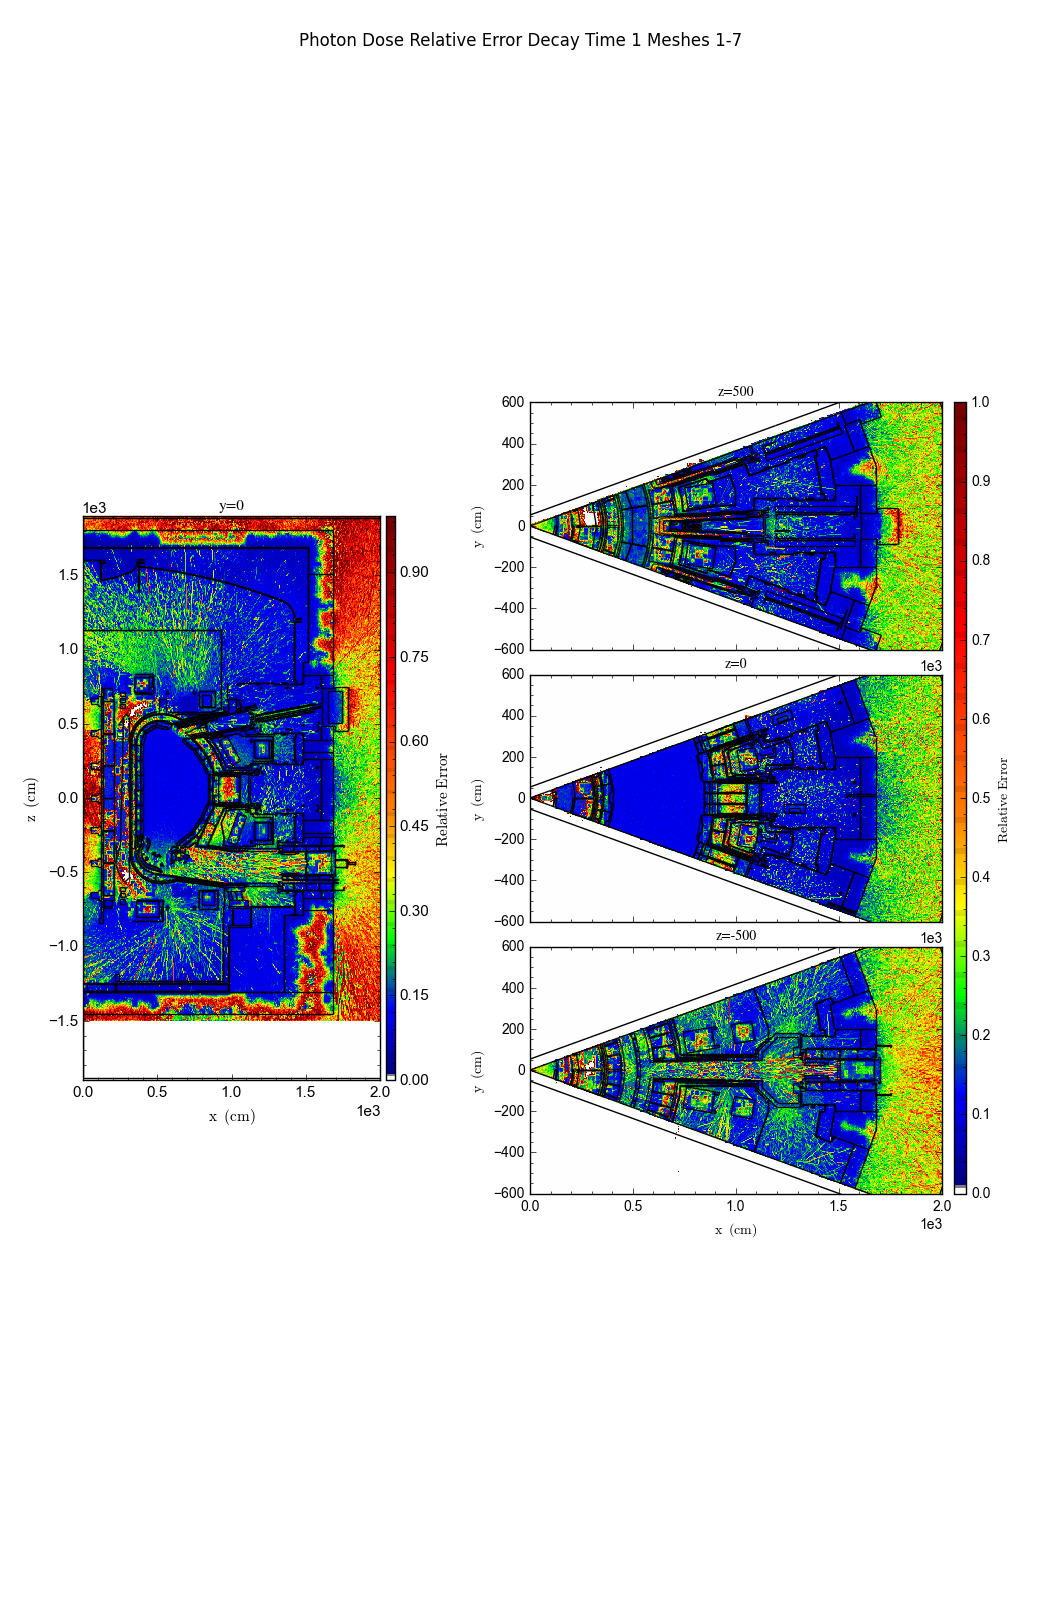
\includegraphics[trim={0cm 8cm, 0cm 8cm},clip,scale=0.75]{../plots/final_model/10year/Photon_Dose_Relative_Error_Decay_Time_1_Meshes_1-7.png}
\caption{Total dose rate relative error for decay time 1 for the ``SA-2 - 5 Yr'' irradiation}
\label{fig:photons_10y_dc1_nob4c_relerr}
\end{figure}
\clearpage
\begin{figure}[ht!]
\centering
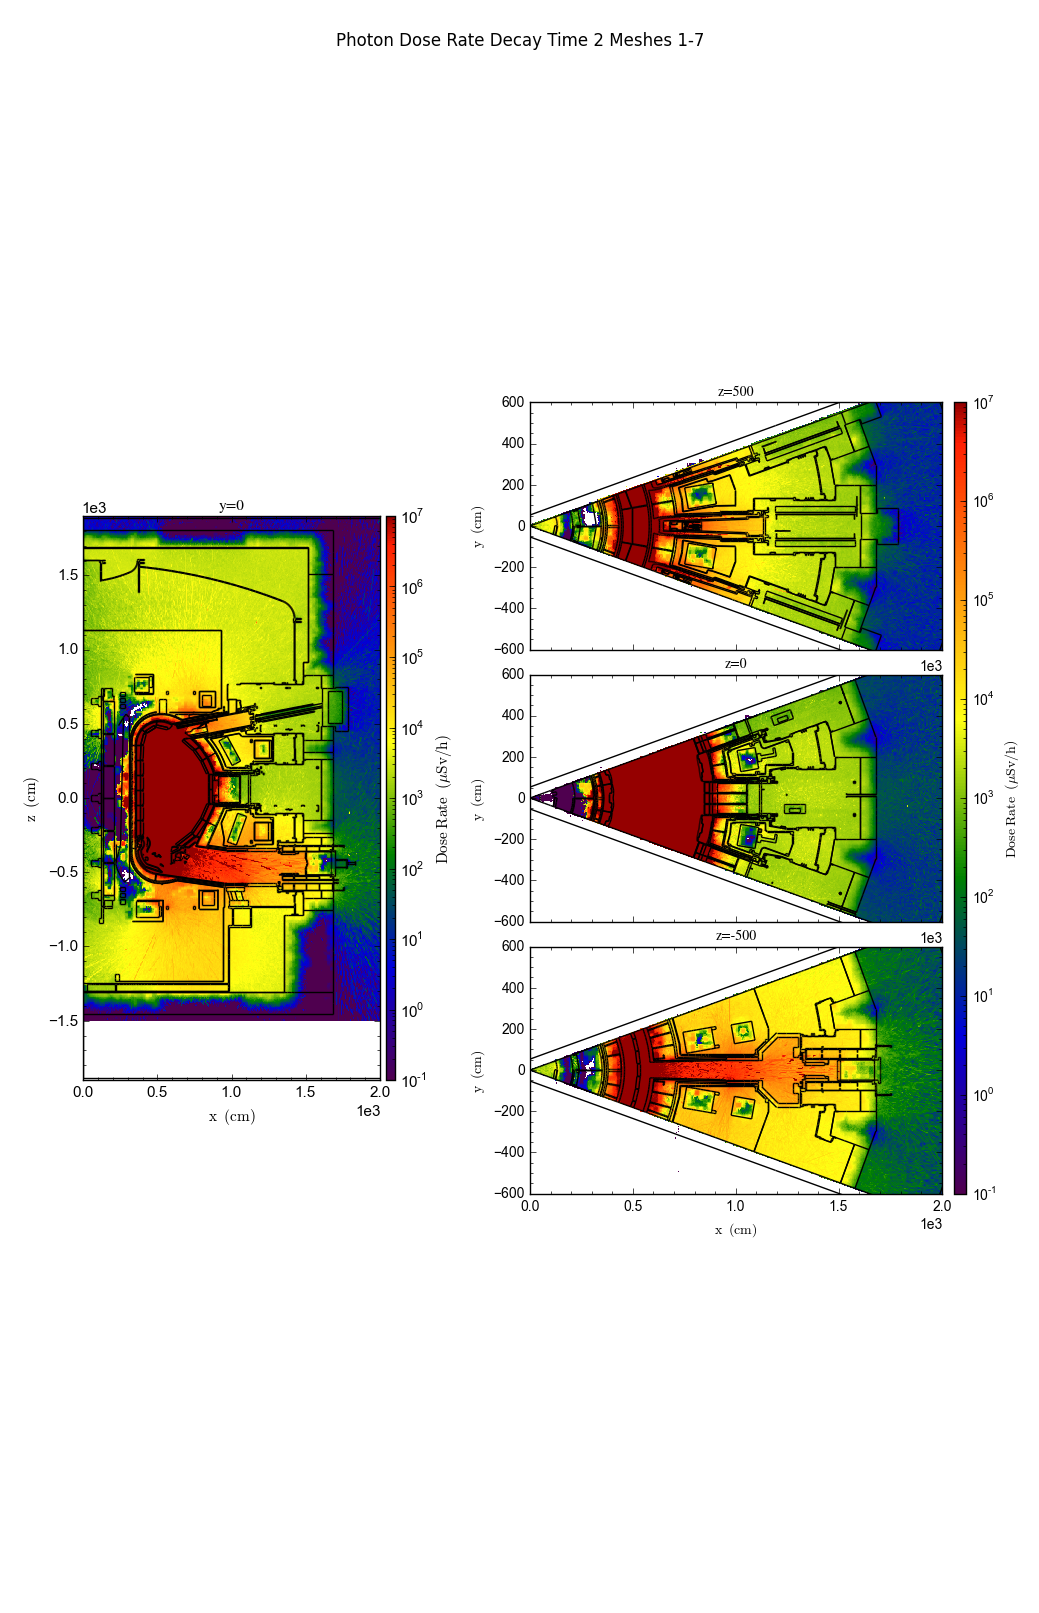
\includegraphics[trim={0cm 8cm, 0cm 8cm},clip,scale=0.75]{../plots/final_model/10year/Photon_Dose_Rate_Decay_Time_2_Meshes_1-7.png}
\caption{Total dose rate for decay time 2 for the ``SA-2 - 5 Yr'' irradiation}
\label{fig:photons_10y_dc2_nob4c_dose}
\end{figure}
\begin{figure}[ht!]
\centering
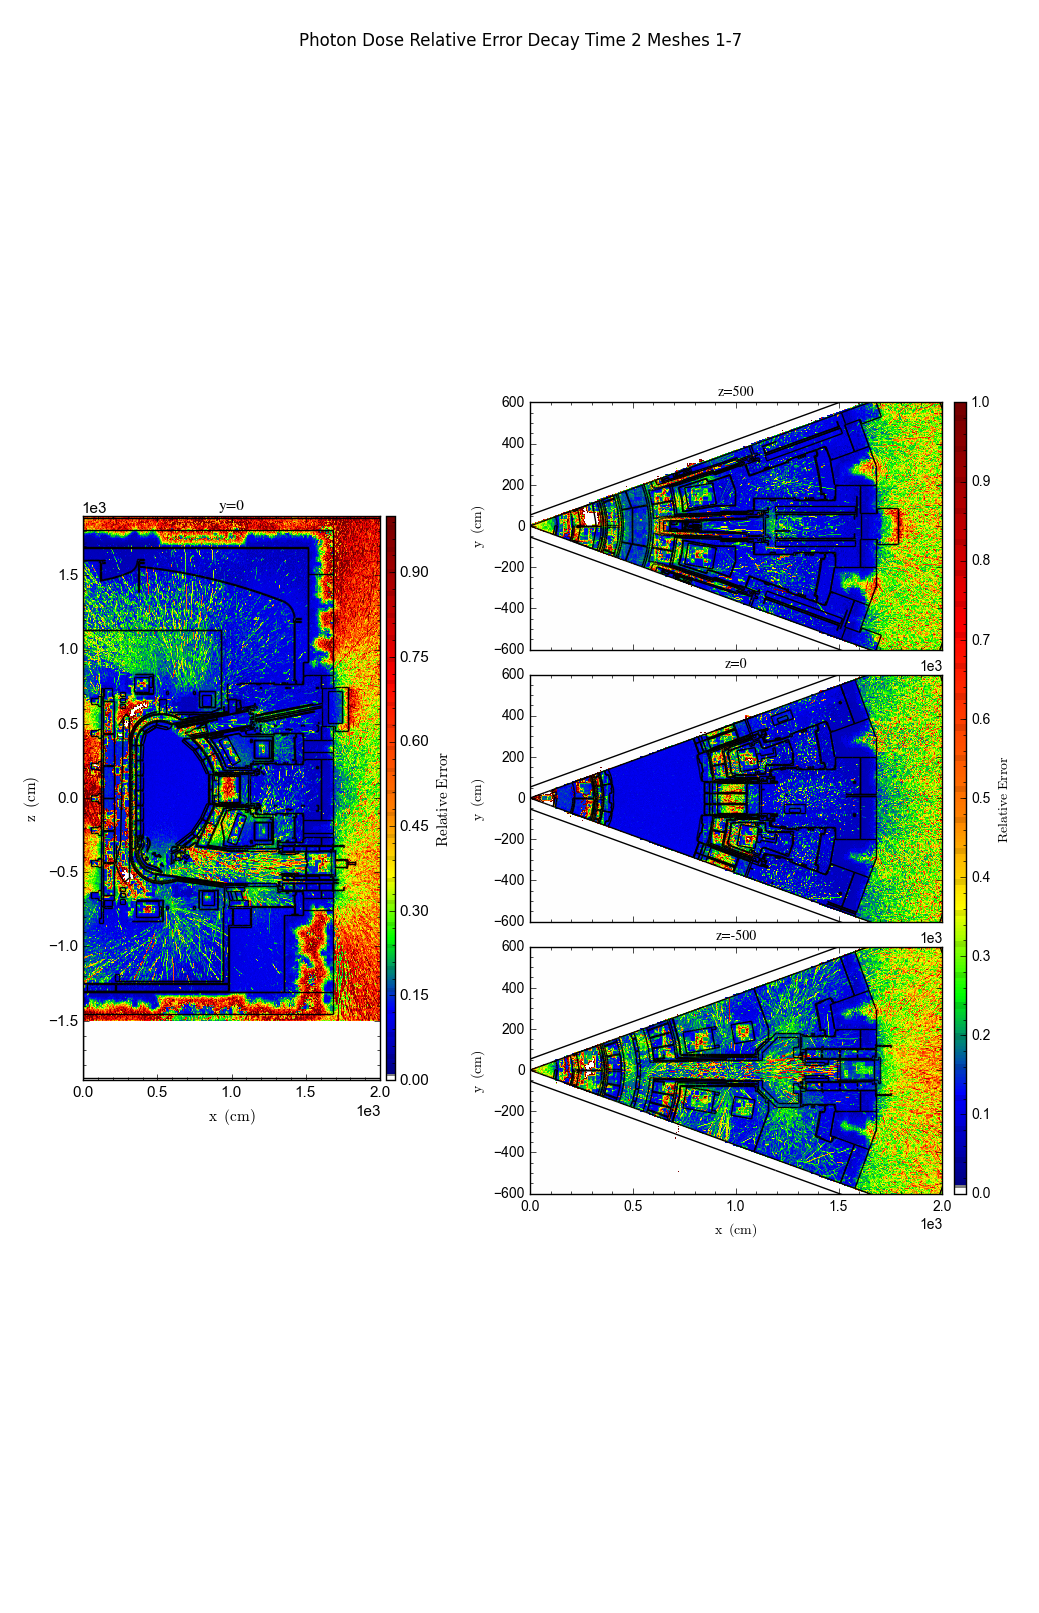
\includegraphics[trim={0cm 8cm, 0cm 8cm},clip,scale=0.75]{../plots/final_model/10year/Photon_Dose_Relative_Error_Decay_Time_2_Meshes_1-7.png}
\caption{Total dose rate relative error for decay time 2 for the ``SA-2 - 5 Yr'' irradiation}
\label{fig:photons_10y_dc2_nob4c_relerr}
\end{figure}

\clearpage
\begin{figure}[ht!]
\centering
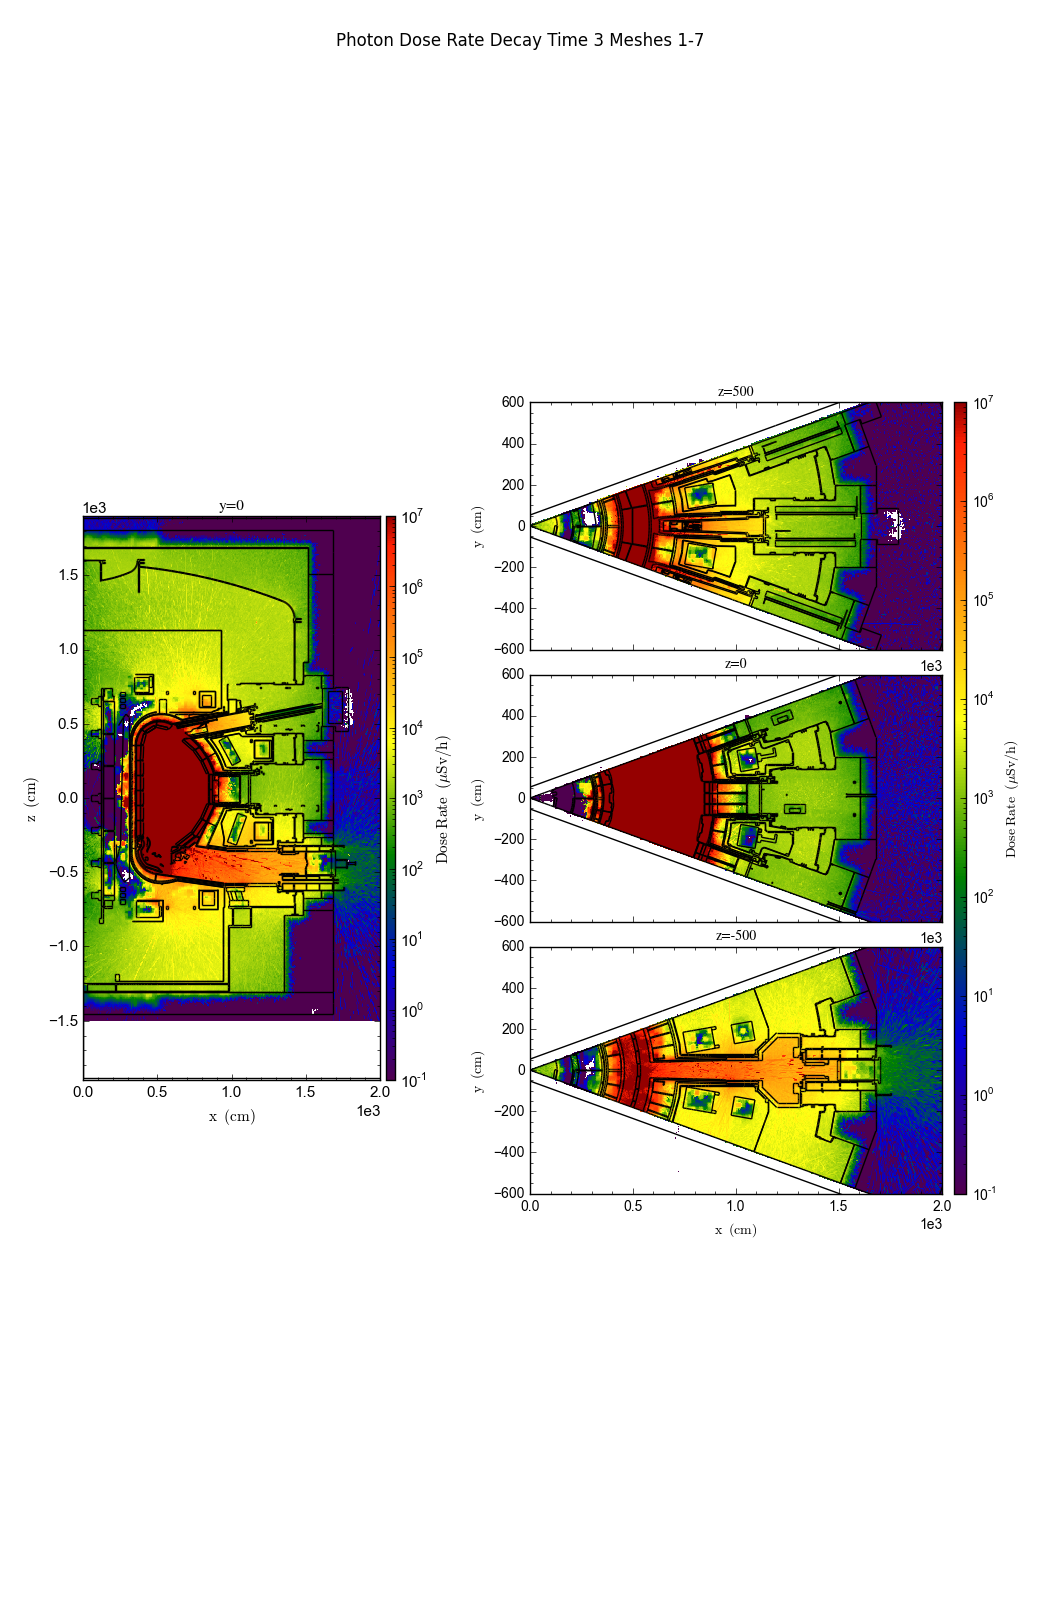
\includegraphics[trim={0cm 8cm, 0cm 8cm},clip,scale=0.75]{../plots/final_model/10year/Photon_Dose_Rate_Decay_Time_3_Meshes_1-7.png}
\caption{Total dose rate for decay time 3 for the ``SA-2 - 5 Yr'' irradiation}
\label{fig:photons_10y_dc3_nob4c_dose}
\end{figure}
\begin{figure}[ht!]
\centering
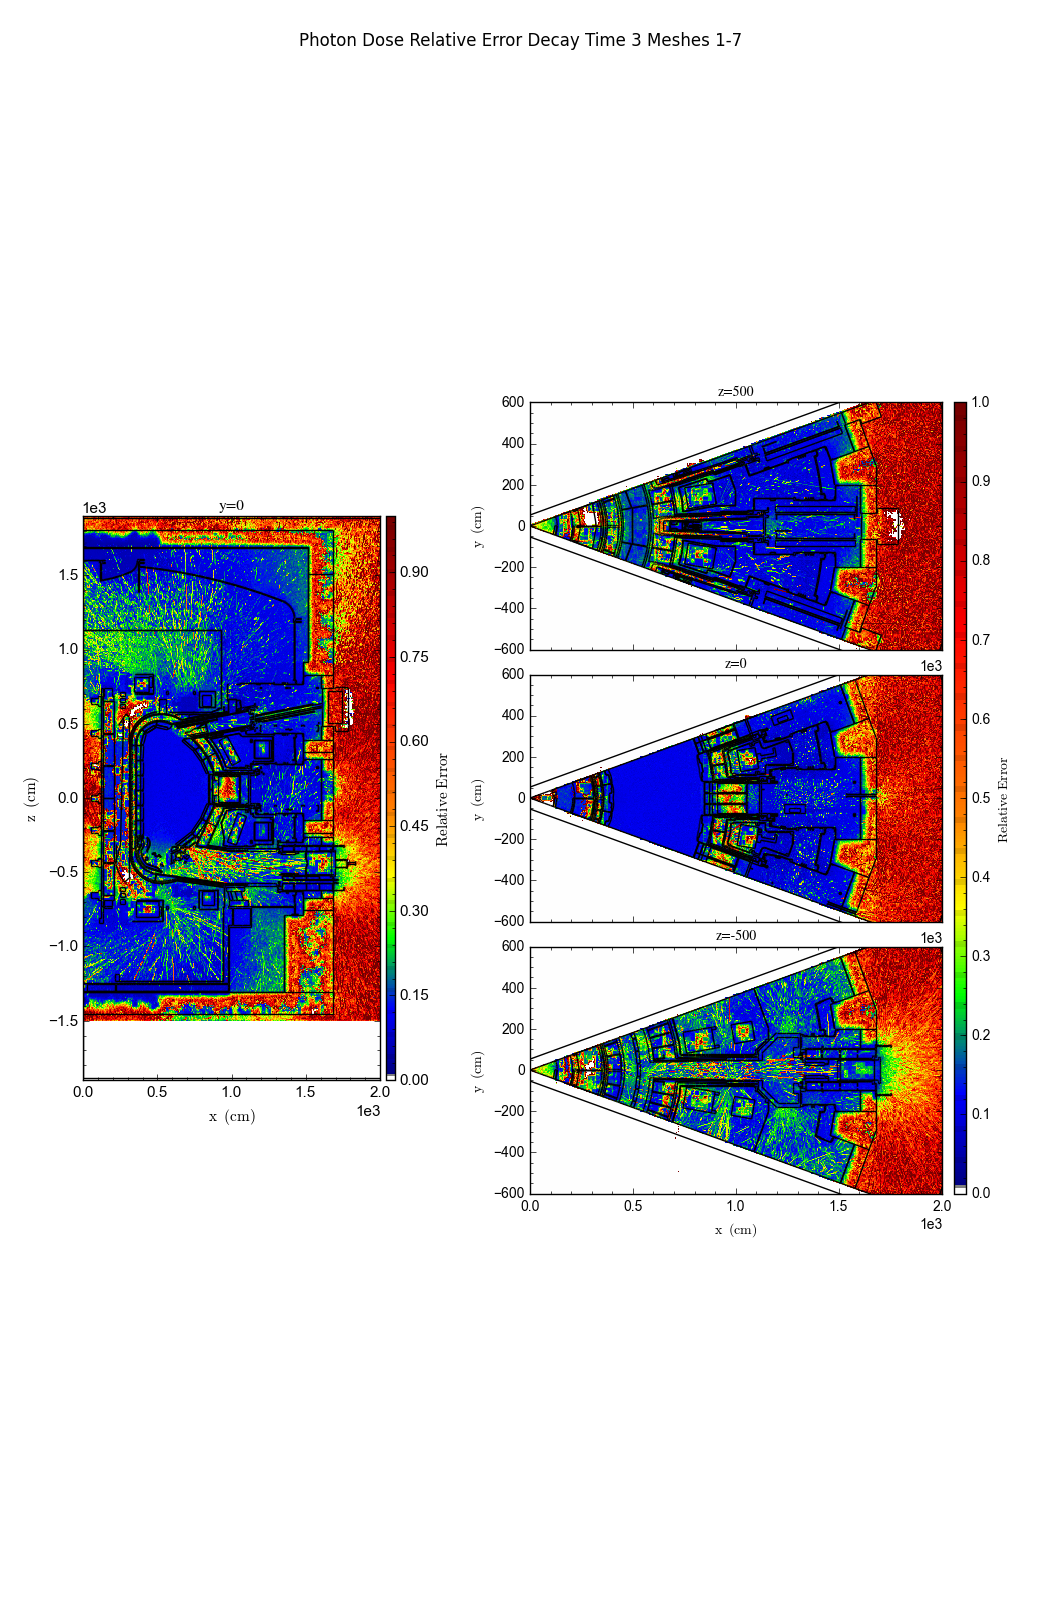
\includegraphics[trim={0cm 8cm, 0cm 8cm},clip,scale=0.75]{../plots/final_model/10year/Photon_Dose_Relative_Error_Decay_Time_3_Meshes_1-7.png}
\caption{Total dose rate relative error for decay time 3 for the ``SA-2 - 5 Yr'' irradiation}
\label{fig:photons_10y_dc3_nob4c_relerr}
\end{figure}

\end{document}
